% !TEX TS-Program = pdflatex

\documentclass[12pt, twoside]{article}

\newcommand{\course}{MA336}

\usepackage{geometry}
\geometry{
    letterpaper,
    left=0.8in,
    top=0.8in,
    headsep=\baselineskip,
    textwidth=26pc,
    marginparsep=2pc,
    marginparwidth=12pc,
    textheight=38\baselineskip,
    headheight=2\baselineskip,
    includemp,
    reversemarginpar,
    bindingoffset=1cm,
    twoside,
    asymmetric
}

\usepackage{amsmath, amsthm}

\usepackage{libertine}  %%%%%The Linux Libertine font family
\usepackage[libertine]{newtxmath}

\usepackage{datetime}
\newdateformat{mydate}{\monthname[\THEMONTH], \THEYEAR}

\newdateformat{lastupdated}
{\THEMONTH/\THEDAY/\THEYEAR}

\newdateformat{semester}{
  \ifthenelse{\THEMONTH=1}{Winter \THEYEAR}{
    \ifthenelse{\THEMONTH<6}{Spring \THEYEAR}{
      \ifthenelse{\THEMONTH>8}{Fall \THEYEAR}{
        Summer \THEYEAR
      }
    }
  }
}

\usepackage{titling}

\renewcommand{\sectionmark}[1]{ \markright{#1}{} }

\usepackage{fancyhdr}
\pagestyle{fancy}

\fancyhf{}
\fancyhfoffset[L]{14pc}

\renewcommand{\headrulewidth}{1pt}
\renewcommand{\footrulewidth}{1pt}
\fancyhead[RE,LO]{\bf \course}
% \fancyhead[RO,LE]{\thepage}
\fancyhead[C]{\large\bf Lecture \leftmark}
\fancyfoot[RE, LO]{\raisebox{-10\baselineskip}{\semester{\thedate}}}
\fancyfoot[RO, LE]{\raisebox{-10\baselineskip}{\hfill \sffamily \theauthor}\hspace{-1ex}}
\fancyfoot[C]{\raisebox{-10\baselineskip}{\thepage}}

\usepackage{ifthen}
\usepackage{xparse}
\usepackage{ifoddpage}

\usepackage{eso-pic}

\NewDocumentCommand{\addBG}{}{
  \AddToShipoutPicture{
    \AtTextLowerLeft{
      \put(-1pc,\LenToUnit{-\baselineskip}){
        \rule[0em]{1.5pt}{\dimexpr \textheight+2\baselineskip}
      }
    }
  }
}

\NewDocumentCommand{\newlecture}{}{
  \newpage
  \checkoddpage
  \ifoddpage
  \else
    \clearpage
    \thispagestyle{empty}
    \ClearShipoutPictureBG
    \cleardoublepage
    \newpage
    \addBG
  \fi
}

\usepackage{graphicx}
\usepackage[
  breaklinks = true,
  colorlinks = true,
  pdftitle = "Statistics Worksheets",
  pdfauthor = "Dr. Ye"
]{hyperref}
\usepackage{bookmark}
\usepackage{longtable}
\usepackage{calc}
\usepackage{booktabs}
\usepackage{array}
\usepackage{multirow}
\usepackage{multicol}
\usepackage{float}
\usepackage{colortbl}
\usepackage{pdflscape}
\usepackage{tabu}
\usepackage{tabularx}
\usepackage{threeparttable}
\usepackage{threeparttablex}
\usepackage[normalem]{ulem}
\usepackage{makecell}
\usepackage{xcolor}

\usepackage{changepage}

\newenvironment{fullwidth}{%
  \begin{adjustwidth}{-14pc}{}%
  \hsize=\linewidth%
}{
  \end{adjustwidth}
}

\usepackage[inline]{enumitem}
\setenumerate{
	label=\textup{(\arabic*)},
	% afterlabel={\quad},
	%%vertical
	topsep=0pt,
	partopsep=0pt,
	itemsep=4\baselineskip,
	parsep=2pt,
  after=\vspace*{\dimexpr 4\baselineskip},
	% labelindent=0em,
	% itemindent = *,
	itemindent=1ex,
	wide,
	itemjoin={\hspace{\fill}},
	%%Horizontal
}
\setitemize{
	%%vertical
	topsep=0pt,
	partopsep=0pt,
	itemsep=0pt,
	parsep=0pt,
	%%Horizontal
	labelindent=0em,
	leftmargin =!,
	itemindent = 0pt,
	labelsep= 2pt,
	labelwidth=1em,
}
\setlist{topsep=0pt}

\SetEnumitemKey{sepno}{nosep, after=\vspace*{0pt}}

\SetEnumitemKey{twocol}{
itemsep = 1\itemsep,
parsep = 1\parsep,
before = \raggedcolumns\begin{multicols}{2},
after = \end{multicols}}

\usepackage{tikz}
\usepackage{pgfplots}
\pgfplotsset{compat=newest}
\usepackage{pgfmath}
\usepackage{tikz-cd}
\usepackage{pgffor}
\usepackage{tkz-euclide}
\usepgfplotslibrary{fillbetween}
\usetikzlibrary{
	calc,
	angles,
	quotes,
	arrows.meta,
	math,
	backgrounds,
	pgfplots.statistics,
	matrix,
	patterns,
	shapes.geometric,
	spy,
    intersections,
    decorations.markings,
    decorations.pathmorphing,
    decorations.pathreplacing,
    decorations.shapes
}
\pgfdeclarelayer{ft}
\pgfdeclarelayer{bg}
\pgfsetlayers{bg,main,ft}
%%%%%%%%%%%%%%%%%%%%%%%%%%%%%%%%%%%%%%%%%%%%%%%%%%%%%%%%%%%%%%%%%%%%

%%%%%%%%%%%%%%%%% Setup the Coordinate System %%%%%%%%%%%%%%%%%%%%%%
\pgfplotsset{every axis/.style={
			%		 axis equal image,
			axis x line=middle,    % put the x axis in the middle
			axis y line=middle,    % put the y axis in the middle
			axis line style={-latex,very thick}, % arrows on the axis
			xlabel={$x$},          % default put x on x-axis
			ylabel={$y$},          % default put y on y-axis
			xlabel style = {font=\tiny, at={(xticklabel* cs:1)}, anchor=south},
			ylabel style = {font=\tiny, at={(yticklabel* cs:1)}, anchor=west},
			scaled ticks=true,
			x tick label style={font=\tiny, yshift=0.25ex, inner xsep=0pt},
			y tick label style={font=\tiny, xshift=0.25ex, inner ysep=0pt},
			grid style={black},
			% set layers=standard,
		}
}

%%%%%%%%%%%%%%% include files/Figure %%%%%%%%%%%%%%%%%%%%%%%%%%%%%%%%%
\usepackage{import}
% \usepackage{subfiles}
\usepackage[verbose]{wrapfig}
%%%%%%%%%%%%%%%%%%%%%%%%%%%%%%%%%%%%%%%%%%%%%%%%%%%%%%%%%%%%%%%%%

%%%%%%%%%%%%%%%% Cancel common factors in Math %%%%%%%%%%%%%%%%%%%%
\usepackage[makeroom]{cancel}
%%%%%%%%%%%%%%%%%%%%%%%%%%%%%%%%%%%%%%%%%%%%%%%%%%%%%%%%%%%%%%%%%%%

%%%%%%%%%%%%%% Math mode without vertical spacing %%%%%%%%%%%%%%%%%
\makeatletter
\g@addto@macro\normalsize{%
	\setlength\abovedisplayskip{1pt plus 2pt minus 2pt}%
	\setlength\belowdisplayskip{1pt plus 2pt minus 2pt}%
	\setlength\abovedisplayshortskip{1pt plus 2pt minus 2pt}%
	\setlength\belowdisplayshortskip{1pt plus 2pt minus 2pt}%
}
\makeatother
%%%%%%%%%%%%%%%%%%%%%%%%%%%%%%%%%%%%%%%%%%%%%%%%%%%%%%%%%%%%%%%%

\newcommand{\ZZ}{\mathbf{Z}}
\newcommand{\RR}{\mathbf{R}}
\newcommand{\NN}{\mathbf{N}}
\newcommand{\QQ}{\mathbf{Q}}
\newcommand{\abs}[1]{\lvert #1\rvert}
\newcommand{\ii}{\mathbf{i}}
\newcommand{\parll}{ {\mathbin{\parallel}} }
\newcommand{\prll}{{\mathbin{\!/\mkern-5mu/\!}}}

\makeatletter
\renewcommand*\rel@kern[1]{\kern#1\dimexpr\macc@kerna}
\renewcommand*\widebar[1]{%
\begingroup
\def\mathaccent##1##2{%
\rel@kern{0.8}%
\overline{\rel@kern{-0.8}\macc@nucleus\rel@kern{0.2}}%
\rel@kern{-0.2}%
}%
\macc@depth\@ne
\let\math@bgroup\@empty \let\math@egroup\macc@set@skewchar
\mathsurround\z@ \frozen@everymath{\mathgroup\macc@group\relax}%
\macc@set@skewchar\relax
\let\mathaccentV\macc@nested@a
\macc@nested@a\relax111{#1}%
\endgroup
}
\renewcommand{\bar}{\widebar}
\newcommand*\centermath[1]{\omit\hfil~$\displaystyle#1$~\hfil\ignorespaces}
\newcommand{\cmc}{\centermath}
\newcommand*\ctc[1]{\omit\hfil\quad~ #1 ~\quad\hfil\ignorespaces}
\newcommand{\dfn}[1]{\textit{\textbf{#1}}}


\theoremstyle{plain}% default
\newtheorem{theorem}{Theorem}[section]
\newtheorem{lemma}[theorem]{Lemma}
\newtheorem{proposition}[theorem]{Proposition}
\newtheorem{corollary}[theorem]{Corollary}
\theoremstyle{definition}
\newtheorem{definition}[theorem]{Definition}
\newtheorem{example}{Example}[section]
\newtheorem{exercise}{Exercise}[section]
\theoremstyle{remark}
\newtheorem*{remark}{Remark}
\newtheorem*{note}{Note}
\newtheorem{case}{Case}



\title{\course~Worksheet}
\author{Dr. Ye}
\date{}

% \date{\semester{\today}}


\begin{document}
\newgeometry{margin=1in}

\clearpage

\ClearShipoutPictureBG

\begin{titlepage}
  \vspace{2\baselineskip}
  
  \maketitle
  
  \thispagestyle{empty}

  \vfill
  \centering{
  \small
  Last updated on \lastupdated{\today}\\
  
  License: \href{CC BY-NC-SA}{https://creativecommons.org/licenses/by-nc-sa/4.0/}
  } 
  \vspace{3\baselineskip}
\end{titlepage}

\newpage
\addBG

\restoregeometry

% !TeX root =  main.tex

\section{Statistical Studies}

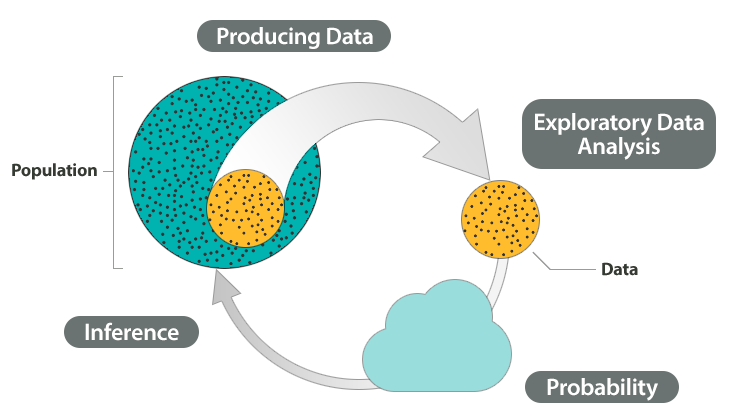
\includegraphics[scale=0.4]{Figures/Big-Picture.png}

\hypertarget{basic-statistical-concepts-14}{%
\subsection{Basic statistical concepts}\label{basic-statistical-concepts-14}}

\begin{itemize}
\item
  \textbf{Data} consists of information from observation, counts,
  measurements, responses or experiments.
\item
  A \textbf{population} is the collection of all objects that are of
  interest.
\item
  A \textbf{parameter} is a number that is a property of the population.
\item
  A \textbf{sample} is a subset of a population.
\item
  A \textbf{statistic} is a number, such as a percentage, that
  represents a property of a sample.
\item In statistics, a \textbf{variable} is a characteristic, or attribute
of interest that we gather about individuals or objects.
\item
  \textbf{Categorical variables} (or qualitative variables) represent
  attributes, labels or nonnumerical entries, such as names, and
  colors.
\item
  \textbf{Quantitative variables} represent numerical measurements or
  counts, such as weights and number of students in each class.
\end{itemize}

\begin{example}
  Identify the population, parameter, sample, and statistic in the following study: \textit{To learn the   percentage of students go to school by public transportation, 500
  students at a college were surveyed. 50\% say they go to school by
  public transportation}
\end{example}
\vspace*{2\baselineskip}

\begin{example}
  Identify the type variables.\\
\begin{enumerate*}
  \item Age
  \item Hair color
  \item GPA
  \item temperature
  \item Education attainment
\end{enumerate*}
\end{example}


\begin{exercise}
Identify the population, sample, the variable of study, the type of the
variable, the population parameter and the sample statistics.

\emph{An administrator wishes to estimate the passing rate of a certain
course. She takes a random sample of 50 students and obtains their
letter grades of that course. Among the 50 students, 32 students earned
a grade C or better.}
\end{exercise}
\vspace*{3\baselineskip}

\hypertarget{types-of-statistical-studies}{%
\subsection{Types of statistical
studies}\label{types-of-statistical-studies}}

  A statistical study can usually be categorized as an
  \textbf{observational study} or an \textbf{experiment} by the mean of
  study.

  \begin{itemize}
  \item
    An observational study observes individuals and measures variables
    of interest. The main purpose of an observational study is to
    describe a group of individuals or to investigate an association
    between two variables.
  \item
    An experiment intentionally manipulates one variable in an attempt
    to cause an effect on another variable. The primary goal of an
    experiment is to provide evidence for a cause-and-effect
    relationship between two variables.
  \end{itemize}

\begin{example}
  Which type of study will answer the question best.

  \begin{enumerate}[itemsep=2\baselineskip]
  \item
    What proportion of all college students in the United States have
    taken classes at a community college?
  \item
    Does use of computer-aided instruction in college math classes
    improve test scores?
  \end{enumerate}
\end{example}

\begin{exercise}
  Identify the type of statistical study:
  \begin{enumerate}[itemsep=2\baselineskip]
  \item
    \emph{A study took random sample of adults and asked them about their
    bedtime habits. The data showed that people who drank a cup of tea
    before bedtime were more likely to go to sleep earlier than those who didn't drink tea.}
  \item
    \emph{Another study took a group of adults and randomly divided them into two groups. One group was told to drink tea every night for a week, while the other group was told not to drink tea that week.
    Researchers then compared when each group fell asleep.}
  \end{enumerate}
\end{exercise}
\vspace*{-2\baselineskip}

\hypertarget{questions-about-population-12}{%
\subsection{Questions about population}\label{questions-about-population-12}}

\begin{longtable}[]{@{}
  >{\raggedright\arraybackslash}p{(\columnwidth - 2\tabcolsep) * \real{0.5000}}
  >{\raggedright\arraybackslash}p{(\columnwidth - 2\tabcolsep) * \real{0.5000}}@{}}
\toprule()
\begin{minipage}[b]{\linewidth}\raggedright
\textbf{Type of Research Question}
\end{minipage} & \begin{minipage}[b]{\linewidth}\raggedright
\textbf{Examples}
\end{minipage} \\
\midrule()
\endhead
\textbf{Make an estimate about the population} (often an estimate about
an \emph{average} value or a \emph{proportion} with a given
characteristic) & What is the \emph{average} number of hours that
community college students work each week? What \emph{proportion} of all
U.S. college students are enrolled at a community college? \\
\textbf{Test a claim about the population} (often a claim about an
\emph{average} value or a \emph{proportion} with a given characteristic)
& Is the \emph{average} course load for a community college student
greater than 12 units? Do the \emph{majority} of community college
students qualify for federal student loans? \\
\textbf{Compare two populations} (often a comparison of population
averages or proportions with a given characteristic) & In community
colleges, do female students have a \emph{higher} GPA than male
students? Are college athletes \emph{more} likely than non-athletes to
receive academic advising? \\
\textbf{Investigate a correlation} between two variables in the
population & Is there a \emph{correlation} between the number of hours high school students spend each week on Facebook and their GPA? Is
academic counseling \emph{associated} with quicker completion of a
college degree? \\
\bottomrule()
\end{longtable}

\begin{exercise}
  Give an example of a research question that involves
  \begin{enumerate}
    \item 
     estimating a characteristic about all students at QCC.
     \item testing a claim of a characteristic about all students at QCC.
     \item investigating a correlation between two variables about all students at QCC.
  \end{enumerate}
\end{exercise}

\hypertarget{question-on-cause-and-effect}{%
\subsection{Question on
cause-and-effect}\label{question-on-cause-and-effect}}

A research question that focuses on a cause-and-effect relationship is common in disciplines that use experiments, such as medicine or psychology.

  \begin{itemize}
  \item
    Does cell phone usage increase the risk of developing a brain tumor?
  \item
    Does drinking red wine lower the risk of a heart attack?
  \end{itemize}

In a study of a relationship between two variables, one variable is
the \textbf{explanatory variable}, and the other is the
\textbf{response variable}.

\begin{example}
  Determine if the question is a cause-and-effect question? What are the
  explanatory and response variables?
  
  \begin{enumerate}[parsep=3\baselineskip]
  \item
    Does use of computer-aided instruction in college math classes improve
    test scores?
  \item
    Does tutoring correlate with improved performance on exams?
  \end{enumerate}
\end{example}
\vspace*{-2\baselineskip}

\begin{exercise}
  A researcher studies the medical records of 500 randomly selected
  patients. Based on the information in the records, he divides the
  patients into two groups: those given the recommendation to take an
  aspirin every day and those with no such recommendation. He reports
  the percentage of each group that developed heart disease.

  Determine whether the study supports the conclusion that taking
  aspirin lowers the risk of heart attacks.
\end{exercise}
\vspace*{3\baselineskip}

\begin{exercise}
  Does higher education attainment lead to higher salary?
\begin{enumerate}[itemsep=2\baselineskip]
\item
  Determine if the question is a cause-and-effect question?
\item
  What are the explanatory and response variables?
\item
  If a student want to study this question, what type of statistical
  study can be used? What kind of conclusion can be drawn?
\end{enumerate}
\end{exercise}



\hypertarget{sampling-plans}{%
\subsection{Sampling plans}\label{sampling-plans}}

To make accurate inference, the sample must be representative of the
population.

\begin{itemize}
\item
  A \textbf{sampling plan} describes exactly how we will choose the
  sample.
\item
  A sampling plan is \textbf{biased} if it systematically favors certain
  outcomes.
\item
  In \textbf{random Sampling}, every individual or object has an equal
  chance of being selected.
\end{itemize}
\vspace*{-\baselineskip}

\hypertarget{methods-of-random-sampling-12}{%
\subsection{Methods of random sampling}\label{methods-of-random-sampling-12}}

\begin{itemize}
\item
  \textbf{Simple random sample}: groups of the same size are randomly
  selected. Table of random numbers, calculator and computer programs are often
  used to generate random numbers.
\item
  \textbf{Stratified random sample}: The population is first split into
  homogeneous groups. Then a same proportion or a same number of subjects from each group are selected randomly.

  \centerline{
    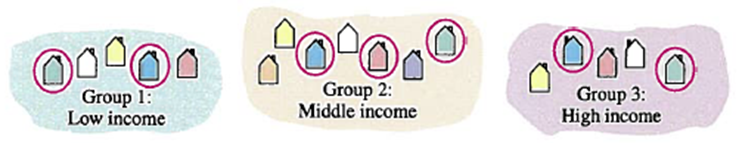
\includegraphics[scale=0.5]{Figures/Stratified-Random-Sample.png}
  }
\item
  \textbf{Cluster sample}: The population is first split into groups. Then some groups are selected randomly.

  \centerline{
    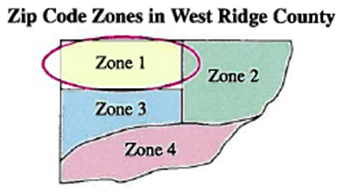
\includegraphics[scale=0.5]{Figures/Cluster-Sample.png}
  }
\item
  \textbf{Systematic sample}: First, a starting number is chosen randomly. Then take every \(n\)-th piece of the data.
  
  \centerline{
    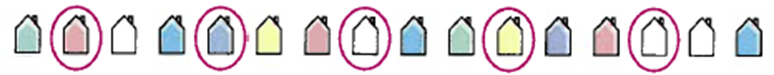
\includegraphics[scale=0.5]{Figures/Systematic-Sample.png}
  }
\end{itemize}

\begin{exercise}
Classify each of the sampling procedures below.

\begin{enumerate}[itemsep=2\baselineskip]
  \item 
  A high school educational researcher interviews 50 high school female teachers and 50 high school male teachers.
  \item The names of 25 employees being chosen out of a hat from a company of 250 employees.
  \item A researcher starts surveying every 10th customer at a local coffee shop starting at a random time between 8 am and 9 am.
  \item A student interviews classmates in his algebra class to determine how many pairs of jeans a student owns, on the average.
\end{enumerate}
\end{exercise}


\hypertarget{bad-sampling}{%
\subsection{Bad sampling}\label{bad-sampling}}

\textbf{Biased sampling}
  \begin{itemize}
  \item
    Online polls. These are examples of a voluntary response sample.
  \item
    Mall surveys. These are an example of a convenience sample.
  \end{itemize}

\textbf{Undercoverage}
  \begin{itemize}
  \item
    It occurs when some groups in the population are left out of the
    process of choosing a sample. For example, random survey math
    students to estimate the average GPA or a college.
  \end{itemize}

\begin{example}
  Suppose that you want to estimate the proportion of students at your
  college that use the library.
  
  Which sampling plan will produce the most reliable results?
  
  \begin{enumerate}[parsep=0pt]
  \item
    Select 100 students at random from students in the library.
  \item
    Select 200 students at random from students who use the Tutoring
    Center.
  \item
    Select 300 students who have checked out a book from the library.
  \item
    Select 50 students at random from the college.
  \end{enumerate}
\end{example}

\begin{exercise}
  Identify the flaw(s) in the study
  
  \textit{Students at an elementary school are given a questionnaire that they are
  asked to return after their parents have completed it. One of the
  questions asked is, ``Do you find that your work schedule makes it
  difficult for you to spend time with your kids after school?'' Of the
  parents who replied, 85\% said ``no''. Based on these results, the
  school officials conclude that a great majority of the parents have no
  difficulty spending time with their kids after school.}
\end{exercise}
\vspace*{2\baselineskip}

\hypertarget{elements-of-experimental-design-12}{%
\subsection{Elements of experimental design}\label{elements-of-experimental-design-12}}

To establish a cause-and-effect relationship, we want to make sure
  that the explanatory variable is the only thing that impacts the
  response variable. We therefore want to get rid of all other factors
  that might affect the response. These factors are called \textbf{confounding variables}.

\begin{itemize}
\item \textbf{Control} reduces the effects of confounding variables. Three control strategies are \textbf{control groups}, \textbf{placebos}, and \textbf{blinding}.

  \begin{itemize}
  \item
    A \textbf{control group} is a baseline group that receives no
    treatment or a neutral treatment.
  \item
    A neutral treatment that has no ``real" effect on the dependent
    variable is called a \textbf{placebo}, and a participant's positive response to a placebo is called the \textbf{placebo effect}.
  \item
    \textbf{Blinding} is the practice of not telling participants
    whether they are receiving a placebo. \textbf{Double-blinding} is the practice of not telling both the participants and the
    researchers which group receiving a treatment or a placebo.
  \end{itemize}

\item
  \textbf{Randomization} ensures that this estimate is statistically
  valid.
  \begin{itemize}
  \item
    With random assignment, we can be fairly confident that any
    differences we observe in the response of treatment groups is due to the explanatory variable.
  \end{itemize}

\item
  \textbf{Replication} reduces variability in experimental results and increases their significance.

  Although randomization helps to insure that treatment groups are as similar as possible, the results of a single experiment, applied to a small number of objects or subjects, should not be accepted without question.

  Any good experiment should be reproducible, and in particular, replication should yield similar results.
\end{itemize}

\begin{example}
  In the study of the relation between a type
  fertilizer and tomato size, the amount of sunshine will be a
  confounding variable. It contributes to the growth of tomato.
\end{example}
\vspace*{2\baselineskip}

\begin{exercise}
  \textit{A company tested their new golf ball by having 20 professional golfers
  each hit 100 shots with the company's new ball and 100 shots with the golfer's current ball (in a random order). The labels were removed, so the golfers didn't know which balls were which. The golfers, on average, hit their shots significantly farther with the new ball.\\  
  The company cites this study in an advertisement claiming that this new
  ball will help all golfers hit farther shots.}
  
  Is the company's claim appropriate? Why?
\end{exercise}
\vspace*{2\baselineskip}

\begin{exercise}
  \textit{Over the years it has been said that coffee is bad for you. When looking at the studies that have shown that coffee is linked to poor health, you will see that people who tend to drink coffee don't sleep much, tend to smoke, don't eat healthy, and tend to not exercise.} 
  
  Can you say that the coffee is the reason for the poor health or are there any confounding variables?
\end{exercise}
\vspace*{5\baselineskip}

\subsection{Lab 1 - Introduction to Excel}

\begin{exercise}
  In the follow figure, highlight the cell C3, the array A1:B2, and the icon for inserting function.

  \centerline{
    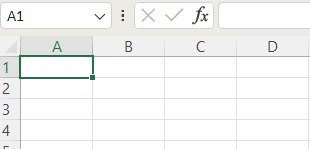
\includegraphics[scale=0.8]{Figures/Excel-CellLocator-Function.png}
  }
\end{exercise}

\begin{exercise}
  Describe how to use the Excel autofill function to generate a sequential array.
\end{exercise}
\vspace*{3\baselineskip}

\begin{exercise}
  Write down two Excel functions that can be used to generate random numbers and describe the difference.
\end{exercise}
\vspace*{3\baselineskip}

\begin{exercise}
  Describe approach on how to use the paste special option to convert a row array into a column array.
\end{exercise}
% \vspace*{3\baselineskip}

% \begin{exercise}
%   Describe how to use autofill to add a number in the cell B1 to each number in the array A1:A10.
% \end{exercise}
\newlecture

% !TeX root = main.tex
\section{Summarizing Data Graphically}

\hypertarget{distribution-of-quantitative-data}{%
\subsection{Distribution of Quantitative
Data}\label{distribution-of-quantitative-data}}

\begin{itemize}
\item
  In data analysis, one goal is to describe \textbf{patterns} (known as
  the \textbf{distribution}) of the variable in the data set and create
  a useful summary about the set.
\item
  To describe patterns in data, we use descriptions of \textbf{shape},
  \textbf{center}, and \textbf{spread}. We also describe exceptions to
  the pattern. We call these exceptions \textbf{outliers}.
\end{itemize}

% \begin{figure}[h!]
  \begin{center}
    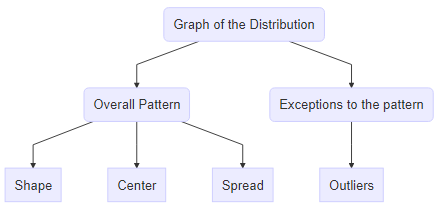
\includegraphics[width=\textwidth]{Figures/Graph-of-Distribution.png}
  \end{center}
% \end{figure}

\hypertarget{dot-plots}{%
\subsection{Dot Plots}\label{dot-plots}}

\begin{itemize}
\item
  A \textbf{dot plot} includes all values from the data set, with one
  dot for each occurrence of an observed value from the set.
\end{itemize}

\begin{example}
The data set contains 15 petal lengths of iris flower. Create a dot plot
to describe the distribution of petal lengths.

1.4, 1.4, 1.3, 1.5, 1.4, 1.7, 1.4, 1.5, 1.4, 1.5, 1.5, 1.6, 1.4, 1.1,
1.2
\end{example}
\vspace*{8\baselineskip}

\begin{exercise}
The data set contains the heights of 20 Black Cherry Trees. Create a dot
plot to describe the distribution of the heights.

64, 69, 71, 72, 74, 74, 75, 76, 76, 77, 78, 80, 80, 80, 80, 81, 82, 85,
86, 87
\end{exercise}
\vspace*{6\baselineskip}

\hypertarget{histograms}{%
\subsection{Histograms}\label{histograms}}

\begin{itemize}
\item
  A \textbf{histogram} divides values of a variable into
  \emph{equal-sized} intervals called \textbf{bins} (classes in some
  books) and uses a rectangular bar to show the \textbf{frequency
  (count)} of observations in each interval.
\item
  A \textbf{frequency distribution} is a table which contains bins,
  frequencies and/or \textbf{relative frequencies} which are proportions
  (percentage) defined by the formula \[
    \text{Relative frequency} =\frac{\text{Class frequency}}{\text{Sample size}}.
  \]
\item
  Each bin has a \textbf{lower bin limit}, which is the left endpoint of
  the interval, and an \textbf{upper bin limit}, which is the right
  endpoint of the interval.
\item
  The \textbf{bin width} is the distance between the lower (or upper)
  bin limits of two consecutive bins.
\item
  The difference between the maximum and the minimum data entries is
  called the \textbf{range}.
\item
  The \textbf{midpoint} of a bin is the half of the sum of the lower and
  upper limits of the bin.
\end{itemize}

\begin{example}
The following data set show the mpg (mile per gallon) of 30 cars.
Construct a frequency table and frequency histogram for the data set
using \(7\) bins.

21, 21, 22.8, 21.4, 18.7, 18.1, 14.3, 24.4, 22.8, 19.2, 17.8, 16.4,
17.3, 15.2, 10.4, 10.4, 14.7, 32.4, 30.4, 33.9, 21.5, 15.5, 15.2, 13.3,
19.2, 27.3, 26, 30.4, 15.8, 19.7
\end{example}
\vspace*{8\baselineskip}

\begin{remark}
\mbox{}
\begin{itemize}
\item
  Avoid histograms with large bin widths and small bin widths.
  \href{https://courses.lumenlearning.com/wmopen-concepts-statistics/chapter/histograms-2-of-4/}{See
  Histogram 2 of 4 in Concepts in Statistics for an interactive
  demonstration}
\item
  When bin width is no given, we may first determine the number of bins.
  If the number of bins is \(k\), then we choose a number with the same
  or one more decimal place that is greater than
  \(\frac{\text{range}}{k}\), but no more than
  \(\frac{\text{range}}{k-1}\) as the bin width. This is to avoid that
  the last bin limit is too much bigger than the max.

  To determine the number of bins, there are some ``rules of thumb''.
  For example, the Rice rule takes the bin number
  \(k = \lceil 2n^{1/3}\rceil\), where \(\lceil 2n^{1/3}\rceil\) is the
  roundup of \(2n^{1/3}\).

  See the
  \href{https://www.statisticshowto.datasciencecentral.com/choose-bin-sizes-statistics/}{Statistic
  How To} page for more discussion on choosing bin width.
\item
  The convenient starting point should not be too much smaller than the
  min. The starting points together with the bin width affects the shape
  of the histogram. It'd be better to experiment with different choices
  of the starting point and the bin width.
\item
  The area of a bar represents the relative frequency for the bin. There
  should be \emph{no space} between any two bars.
\end{itemize}

\end{remark}

\begin{exercise}
The following data set show the petal length of 20 irises. Construct a
frequency table and frequency histogram for the data set using 6 bins.

1.4, 5.4, 1.2, 4.5, 6.1, 1.5, 4.7, 1.4, 5.6, 5.2, 1.3, 6.3, 5.1, 5.6, 5,
6.7, 1.4, 1.6, 1.5, 1.5
\end{exercise}
\vspace*{8\baselineskip}

\hypertarget{common-descriptions-of-shape-distribution}{%
\subsection{Common Descriptions of Shape
Distribution}\label{common-descriptions-of-shape-distribution}}

\begin{itemize}
\item
  \textbf{Right skewed} (or reverse \(J\)-shaped): A right-skewed
  distribution has a lot of data at lower variable values. (Example: the
  histogram example.)
\item
  \textbf{Left skewed} (or \(J\)-shaped): A left skewed distribution has
  a lot of data at higher variable values with smaller amounts of data
  at lower variable values.
\item
  \textbf{Symmetric with a central peak (or bell-shaped)}: A central
  peak with a tail in both directions. A bell-shaped distribution has a
  lot of data in the center with smaller amounts of data tapering off in
  each direction. (Example: the petal length example.)
\item
  \textbf{Uniform}: A rectangular shape, the same amount of data for
  each variable value.
\end{itemize}

\begin{exercise}
Statistics are used to compare and sometimes identify authors. The
following lists shows a simple random sample that compares the letter
counts for three authors.

Terry: 7, 9, 3, 3, 3, 4, 1, 3, 2, 2

Davis: 3, 4, 4, 4, 1, 4, 5, 2, 3, 1

Maris: 2, 3, 4, 4, 4, 6, 6, 6, 8, 3

Create a dot plot for each sample and describe the shape of the
distribution of each sample.
\end{exercise}
\vspace*{5\baselineskip}

\hypertarget{measure-of-centers}{%
\subsection{Measure of Centers}\label{measure-of-centers}}

\begin{itemize}
\item
  \textbf{Mean}: The mean is the average, this is the quotient of the
  total sum by the total number.
\item
  \textbf{Median}: The median is a value that separate the data into the
  lower half and the upper half. To calculate the median, sort the data
  first. If the number of data values is odd, the median is the middle
  value. Otherwise, the median is the mean of the middle two values.
\item
  \textbf{Mode}: The mode is the value that has the most occurrence in
  the data set.
\item
  Use the \emph{mean} as a measure of center only for distributions that
  are \emph{reasonably symmetric} with a central peak. When outliers are
  present, the mean is not a good choice.
\item
  Use the \emph{median} as a measure of center for all \emph{other
  cases}.
\item
  We need to use a graph to determine the shape of the distribution. So
  graph the data first.
\end{itemize}
\vspace*{-\baselineskip}

\begin{exercise}
A student survey was conducted at a major university. The following
histogram shows distribution of alcoholic beverages consumed in a
typical week. 

1. What is the typical number of drinks a student has
during a week? 

2. Do the data suggest that drinking is a problem in this
university?

\begin{fullwidth}
\begin{center}
  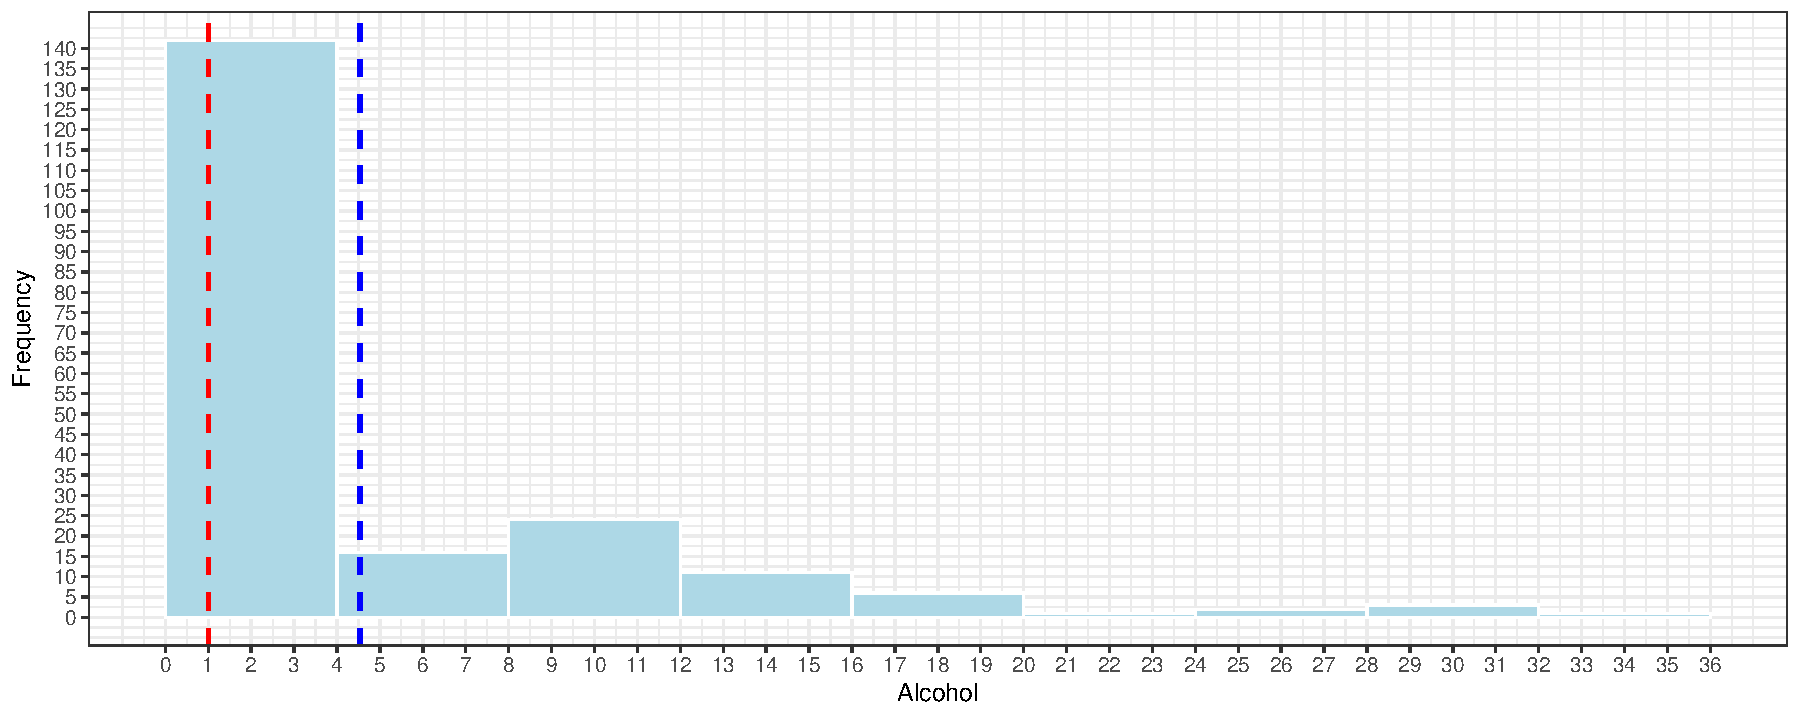
\includegraphics[width=\linewidth]{figure-latex/unnamed-chunk-2-6-1}
\end{center}
\end{fullwidth}
\end{exercise}
\vspace*{5\baselineskip}

\hypertarget{pie-charts}{%
\subsection{Pie Charts}\label{pie-charts}}

\begin{itemize}
\item
  A \textbf{pie chart} is a pie with sectors represents categories and
  the area of each sector is proportional to the frequency of each
  category.

  \begin{itemize}
  \item
    The \textbf{frequency} of a category is the number of occurrences of
    elements in the category.
  \item
    The proportion of a frequency to the size of the population or the
    sample is also called the \textbf{relative frequency}.
  \end{itemize}
\end{itemize}

\begin{example}
The counts of majors of 100 students in a sample are shown in the table.
Use a pie chart to organize the data.

\begin{table}[h!]
  \begin{small}
      \begin{tabular}[c]{l|l}
        \hline
        \multicolumn{1}{c}{\textbf{Grade}} & 
        \multicolumn{1}{c}{\textbf{Frequency (Counts)}} \\
        \hline
        Art & 30 \\
        Engineering & 50 \\
        Science & 20 \\
        \hline
      \end{tabular}
  \end{small}
\end{table}
\end{example}
\vspace*{5\baselineskip}

\begin{exercise}
The following data table summarize passengers on Titanic. Using a pie
chart to describe the data table.

\begin{table}[h!]
  \begin{small}
      \begin{tabular}[c]{l|l}
        \hline
        \multicolumn{1}{c}{\textbf{Class}} & 
        \multicolumn{1}{c}{\textbf{Passengers}} \\
        \hline
        1st & 325 \\
        2nd & 285 \\
        3rd & 706 \\
        Crew & 885 \\
        \hline
      \end{tabular}
  \end{small}
\end{table}

\end{exercise}
\vspace*{5\baselineskip}


\hypertarget{lab-2-summarizing-data-graphically}{%
\subsection{Lab 2: Summarizing Data
Graphically}\label{lab-2-summarizing-data-graphically}}

\hypertarget{create-frequency-tables}{%
\subsubsection{Create Frequency Tables}\label{create-frequency-tables}}

In Excel, to create a frequency table for a data array, we need a bin
array which is used to split the date set into smaller intervals. The
values in a bin array in Excel are (upper) boundaries of intervals. With
a data array and a bin array, we can use the Excel function
\textsf{FREQUENCY\ (data\_array,\ bins\_array)} to create a frequency
table.

Suppose the data set is in column A and the bin array is in column B.
Here is how to create a frequency table using the function
\textsf{FREQUENCY\ (data\_array,\ bins\_array)}:

\begin{enumerate}[sepno]
\item
  In column C, right to the smallest value of the bin array enter
  \textsf{=FREQUENCY(}
\item
  select the data values
\item
  in the formula bar, enter the symbol comma \textsf{,}
\item
  select the bin array
\item
  in the formula bar, enter \textsf{)}.
\end{enumerate}

Hit the \textsf{Enter}, you will get a frequency table.

\begin{remark}

\begin{enumerate}[sepno]
\item
  In this formula, the values in a bin array should be first \(k-1\)
  upper class limits (or the last \(k-1\) lower class limits), where
  \(k\) is the number of bins. In Excel, if the bin array consists of
  30, 40, and 50, then the bins will be \((-\infty,30]\), \((30,40]\),
  \((40, 50]\), \((50, \infty)\).
\item
  In older version of Excel, you may have to highlight cells for
  frequencies first, enter the \textsf{FREQUENCY} function secondly, and
  then hit \textsf{Ctrl+Shift+Enter} (or \textsf{Cmd+Shift+Enter} on
  Mac).
\end{enumerate}

\end{remark}

\begin{exercise}
  Create a frequency table for the following data using the bin width 10.

  31, 32, 32, 33, 35, 36, 37, 37, 38, 38, 39, 40, 40, 40, 42, 42, 43, 43, 45, 45, 46, 47, 48, 48, 51, 55, 55, 56, 60, 60, 61, 66
\end{exercise}
\vspace*{6\baselineskip}

\hypertarget{creating-charts-in-excel}{%
\subsubsection{Creating Charts in Excel}\label{creating-charts-in-excel}}

Excel has many built-in chart functions. To create a charts,

\begin{enumerate}[sepno]
\item
  Select the data array/table
\item
  Under the \textsf{Insert} tab, click on an appropriate chart in the
  \textsf{Charts} command set.
\end{enumerate}

The appearance of chart can be changed after being created.

\begin{exercise}
  The counts of majors of 50 students in a sample are shown in the table.
Use a pie chart to organize the data.

\begin{tabular}[c]{l|l}
  \hline
  \multicolumn{1}{c}{\textbf{Grade}} & 
  \multicolumn{1}{c}{\textbf{Count}} \\
  \hline
  Art & 10 \\
  Engineering & 25 \\
  Mathematics & 15 \\
  \hline
\end{tabular}

\end{exercise}

\vspace*{6\baselineskip}

\hypertarget{create-histogram-charts-in-excel}{%
\subsubsection{Create a Histogram in
Excel}\label{create-histogram-charts-in-excel}}

\begin{enumerate}[sepno]
\item
  Select the data
\item
  On the \textsf{Insert} tab, in the \textsf{Charts} group, from the
  \textsf{Insert\ Statistic\ Chart} dropdown list, select
  \textsf{Histogram}:

  \textbf{Note:} The histogram contains a special first bin which always
  contains the smallest number. This is different from many textbooks.
\end{enumerate}

To \textbf{format the histogram chart} is similar to format a Pie chart.
For example, you can change bin width from \textsf{Format\ Axis}.

\begin{enumerate}[sepno]
\item
  Right-click on the horizontal axis and choose \textsf{Format\ Axis} in
  the popup menu:
\item
  In the \textsf{Format\ Axis} pane, on the \textsf{Axis\ Options} tab,
  you may try different options for bins.
\end{enumerate}

\begin{remark}

\begin{itemize}
\item
  Excel using a different convention to create histogram. The first bin
  is a closed interval and other bins are left open and right closed
  intervals.
\item
  Select the \textbf{Overflow bin} checkbox and type the number, all
  values above this number will be added to the last bin.
\item
  Select the \textbf{Underflow bin} checkbox and type the number, all
  values below and equal to this number will be added to the first bin.
\item
  Histograms show the shape and the spread of quantitative data. For
  categorical data, discrete by its definition, bar charts are usually
  used to represent category frequencies.
\end{itemize}

\end{remark}

\hypertarget{create-histogram-charts-in-excel-using-the-analysis-toolpak}{%
\subsubsection{\texorpdfstring{Create Histogram Charts in Excel using the
\textsf{Analysis\ ToolPak}}{Create Histogram Charts in Excel using the Analysis ToolPak}}\label{create-histogram-charts-in-excel-using-the-analysis-toolpak}}

Suppose your data set is in \textsf{Column\ A} in Excel.

\begin{itemize}
\item
  In the cell \textsf{B1}, put the \emph{first lower bin limit}, which
  is a number slightly less than the minimum but has more decimal places
  than the data set.
\item
  Create upper bin limits in column C.
\item
  In Data menu, look for the Data Analysis ToolPak (if not, go to File
  $\rightarrow$ Options $\rightarrow$ Add-ins $\rightarrow$ Manage
  Excel Add-ins, check Analysis ToolPak). In the popup windows, find
  Histogram.
\item
  In the input range, select your data set. In the bin range, select
  upper bins.
\item
  Check Chart Output and hit OK. You will see the frequency table and
  histogram in Sheet 2.
\item
  Change the gap between bars. Right click a bar and choose
  \textsf{Format\ Data\ Series...} and change the \textsf{Gap\ Width} to
  2\% or 1\%.
\end{itemize}

\hypertarget{how-to-create-a-dotplot-in-excel}{%
\subsubsection{How to Create a Dotplot in
Excel}\label{how-to-create-a-dotplot-in-excel}}

\begin{itemize}
\item
  If you have a raw data set, follow the same procedure a creating a
  histogram but with a bin width equal the same accuracy of the data.
  For example, if you data set consists of integers, then choose 1 as
  the bin-width.
\item
  Change the format of bars in the histogram.

  \begin{itemize}
  \item
    Right click a bar and select \textsf{Format\ Data\ Series...}.
  \item
    Find \textsf{Fill\ \&\ Line} and select both
    \textsf{Picture\ or\ texture\ fill} and
    \textsf{Stack\ and\ Scale\ with}.
  \item
    Click the button \textsf{Online...} and input \emph{dot} in
    \textsf{search\ bing} and hit enter.
  \item
    Select a picture you like and you will get a dot-plot. 
  \end{itemize}
\end{itemize}

\begin{exercise}
Use Excel to complete the following tasks:
\begin{enumerate}[sepno]
\item
  Create a random sample of 30 two-digit integers.
\item
  Create a histogram with 6 bins for the sample.
\item
  Describe the shape of the distribution of the sample of 30 two-digit
  integers.
\end{enumerate}
\end{exercise}
\newlecture

% !TeX root = main.tex

\section{Measure of Center and Variation}

\hypertarget{median-quartiles-interquartile-range-and-outliers}{%
\subsection{Median, Quartiles, Interquartile Range and
Outliers}\label{median-quartiles-interquartile-range-and-outliers}}

\begin{itemize}
\item
  The three \textbf{quartiles}, \(Q_1\), \(Q_2\), and \(Q_3\) are
  numbers in an ordered data set that divide the data set into four
  equal parts. The second quartile is known as the \textbf{median}.
\item
  \textbf{Interquartile Range (IQR for short)} is the measure of
  variation when using the median to measure center. It is defined as
  the difference of the third and the first quartiles:
  \(\text{IQR}=Q_3-Q_1\).
\item
  When the center and the spread are measured by the median and the IQR,
  a value in the data is considered an \textbf{outlier} if the value is

  \begin{itemize}
  \item
    less than the lower fence
    \(\text{fence}_{lower}=Q_1 - 1.5 \cdot \text{IQR}\) or
  \item
    greater than the upper fence
    \(\text{fence}_{upper}=Q_3 + 1.5 \cdot \text{IQR}\).
  \end{itemize}

  \textbf{Note:} An outlier in this definition is also called a
  \textbf{mild outlier}. An outlier that is less than the extreme lower
  fence \(\text{extreme fence}_{lower}=Q_1 - 3 \cdot \text{IQR}\) or
  greater than the extreme upper fence
  \(\text{extreme fence}_{upper}=Q_3 + 3 \cdot \text{IQR}\) is also
  called \textbf{extreme outlier}.
\item
  The minimum, \(Q_1\), \(Q_2\), \(Q_3\) and maximum are known as the
  ``\textbf{five-number summary}'' of the data set.
\item
  The difference of maximum and minimum is called the \textbf{range}.
\end{itemize}

\begin{example}

Find the median, quartiles, IQR and outliers (if they exist) of the
sample height of 15 trees.

70, 65, 63, 72, 81, 83, 66, 75, 80, 75, 79, 76, 76, 69, 75

\end{example}
\vspace*{8\baselineskip}

\begin{exercise}

Find the five-number summary, the IQR and the Range for the following
set of data.

2, 7, 7, 7, 10, 11, 14, 17, 18, 20

\end{exercise}
\vspace*{6\baselineskip}

\hypertarget{box-plot}{%
\subsection{Box Plot}\label{box-plot}}

\begin{itemize}
\item
  A \textbf{box plot} shows a ``five-number summary'' of the data set.
  It contains a box, two whiskers and dots (for outliers).
\item
  To create the boxplot for a distribution,

  \begin{itemize}
  \item
    Draw a box from \(Q_1\) to \(Q_3\).
  \item
    Draw a vertical line in the box at the median.
  \item
    Extend a tail from \(Q_1\) to the smallest value that is not an
    outlier and from \(Q_3\) to the largest value that is not an
    outlier.
  \item
    Indicate outliers with a solid dot.
  \end{itemize}
\end{itemize}

\begin{example}
  Create the boxplot for the ages of 32 best actor oscar winners
  (1970--2001).
  
  31, 32, 32, 33, 35, 36, 37, 37, 38, 38, 39, 40, 40, 40, 42, 42, 43, 43,
  45, 45, 46, 47, 48, 48, 51, 55, 55, 56, 60, 60, 61, 76
\end{example}
\vspace*{6\baselineskip}

\begin{exercise}

Based on the boxplot below, identify the 5 number summary (minimum,
lower quartile (Q1), median (Q2), upper quartile (Q3), maximum)
\begin{fullwidth}
  \begin{center}
    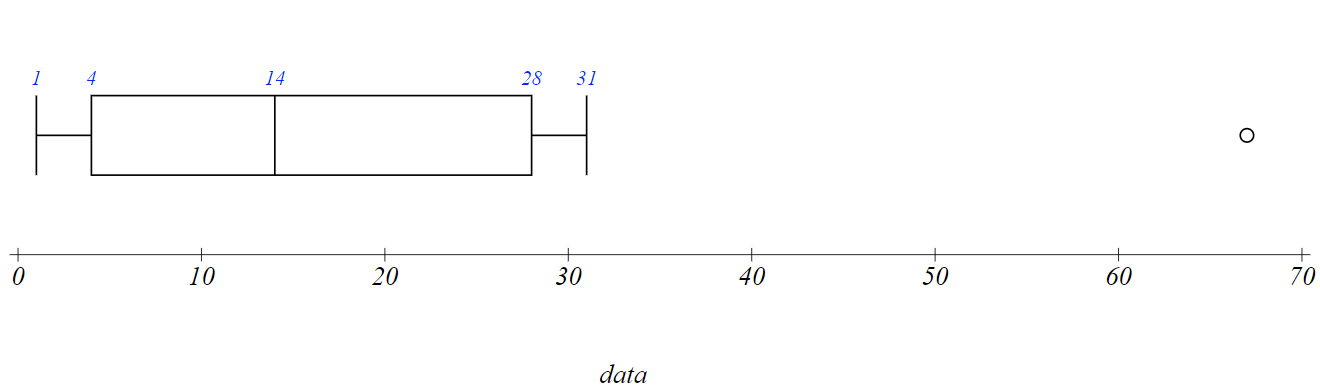
\includegraphics[width=0.9\linewidth]{Figures/Summary-Boxplot.png}
  \end{center}
\end{fullwidth}

\end{exercise}
\vspace*{6\baselineskip}

\hypertarget{mean-and-standard-deviation}{%
\subsection{Mean and Standard
Deviation}\label{mean-and-standard-deviation}}

\begin{itemize}
\item
  Sigma notation: in math, we denote the sum of values \(x_1\), \(x_2\),
  \(\dots\), \(x_n\) of a variable \(x\) by \(\sum\limits_{i=1}^n x_i\)
  or simply by \(\sum x\).
\item
  The \textbf{population mean} is \(\mu= \frac{\sum x}{N}\), where \(N\)
  is the \textbf{population size}, i.e the number of elements in the
  population.

  The notation \(\mu\) reads as mu.
\item
  The \textbf{sample mean} is \(\bar{x}=\frac{\sum{x}}{n}\), where \(n\)
  is the \textbf{sample size}. The notation \(\bar{x}\) reads as
  \(x\)--bar.
\end{itemize}

\begin{example}

Find the mean city mpg for a sample of 10 cars.

18, 21, 20, 21, 16, 18, 18, 18, 16, 20

\end{example}
\vspace*{6\baselineskip}

\hypertarget{weighted-mean}{%
\subsection{Weighted Mean}\label{weighted-mean}}

\begin{itemize}
\item
  The weighted mean of a set of numbers \(\{x_1, \dots, x_n\}\) with
  weights \(w_1\), \(w_2\), \ldots, \(w_n\) is defined as
  \[\frac{\sum w_ix_i}{\sum w_i}.\]
\item
  The mean of a frequency table is weighted mean
  \(\bar{x}=\frac{\sum f x}{n}\), where \(x\) is an element with
  frequency \(f\) and \(n\) is the sample size.
\end{itemize}

\begin{example}

In a course, the overall grade is determined in the following way: the
homework average counts for 10\%, the quiz average counts for 10\%, the
test average counts 50\% , and the final exam counts for 30\%. What's
the overall grade of the student who earned 92 on homework, 95 on
quizzes, 90 on tests and 93 on the final.

\end{example}
\vspace*{6\baselineskip}

\begin{exercise}

Find the average petal width for a sample of 10 iris followers.

0.2, 2.1, 0.2, 1.7, 2.3, 0.3, 1.2, 0.2, 1.8, 2.3

\end{exercise}
\vspace*{6\baselineskip}

\begin{exercise}

Find the mean and median from the dot plot of sepal length for a sample
of 10 iris flowers.

\begin{fullwidth}
  \begin{center}
    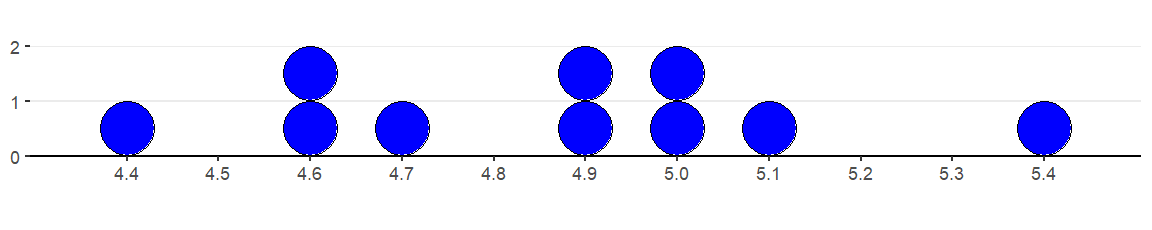
\includegraphics[width=0.8\linewidth]{Figures/MeanMedian-from-Dotplot.png}
  \end{center}
\end{fullwidth}

\end{exercise}
\vspace*{6\baselineskip}

\begin{exercise}

In a student's chemistry class, the final grade is based on six
categories.

The categories, grades, and weights are shown in this table.

\begin{longtable}[]{@{}lll@{}}
\toprule()
Category & Grade & Weight \% \\
\midrule()
\endhead
Test 1 & 46 & 20 \\
Test2 & 61 & 20 \\
Test 3 & 45 & 15 \\
Homework & 72 & 9 \\
Semester Project & 53 & 8 \\
Final Exam & 77 & 28 \\
\bottomrule()
\end{longtable}

Compute a weighted average to determine the student's overall final
grade in the course. Record the overall final grade below as a
percentage. Round accurately to two decimal places.

\end{exercise}
\vspace*{6\baselineskip}

\hypertarget{measure-of-variation-about-population-mean}{%
\subsection{Measure of Variation about Population
Mean}\label{measure-of-variation-about-population-mean}}

\begin{itemize}
\item
  The \textbf{deviation} of an entry \(x\) in a population data set is
  the difference \(x-\mu\), where \(\mu\) is the mean of the population.
\item
  The \textbf{population variance} of a population of \(N\) entries is
  defined as \[
    \text{VAR.P}=\sigma^2=\dfrac{\sum(x-\mu)^2}{N}.
  \]
\item
  The \textbf{population standard deviation} is \[
    \text{STDEV.P}=\sigma=\sqrt{\dfrac{\sum(x-\mu)^2}{N}}.
  \]
\end{itemize}

\hypertarget{measure-of-variation-about-sample-mean}{%
\subsection{Measure of Variation about Sample
Mean}\label{measure-of-variation-about-sample-mean}}

\begin{itemize}
\item
  The \textbf{deviation} of an entry \(x\) in a sample data set is the
  difference \(x-\bar{x}\), where \(\bar{x}\) is the mean of the sample.
\item
  The \textbf{sample variance} and \textbf{sample standard deviation}
  are defined similarly \[
    \text{VAR.S}=s^2=\dfrac{\sum(x-\bar{x})^2}{n-1}, \qquad
    \text{STDEV.S}=s=\sqrt{\dfrac{\sum(x-\bar{x})^2}{n-1}},
  \] where \(n\) is the sample size.
\item
  \textbf{Rounding rule:} for mean, variance and standard deviation, we
  keep at least one more digit than the accuracy of the data set.
\end{itemize}

\textbf{Note:} To measure the spread, one may also use the \textbf{mean
absolute deviation} \[MAD=\dfrac{\sum |x-\bar{x}|}{n}.\] However, the
standard deviation has better properties in applications.

\begin{example}

Find the mean and standard deviation ages of a sample of 32 best actor
oscar winners (1970--2001).

31, 32, 32, 33, 35, 36, 37, 37, 38, 38, 39, 40, 40, 40, 42, 42, 43, 43,
45, 45, 46, 47, 48, 48, 51, 55, 55, 56, 60, 60, 61, 76

\end{example}
\vspace*{6\baselineskip}

\begin{exercise}

A \emph{sample} of GPAs from ten students random chosen from a college
are recorded as follows.

1.90, 3.00, 2.53, 3.71, 2.12, 1.76, 2.71, 1.39, 4.00, 3.33

Find the standard deviation of this sample.

\end{exercise}
\vspace*{6\baselineskip}

\hypertarget{mean-and-standard-deviation-under-linear-transformation}{%
\subsection{Mean and Standard Deviation under Linear
Transformation}\label{mean-and-standard-deviation-under-linear-transformation}}

\begin{itemize}
\item
  When we increase values in a data set by a fixed number \(c\), the
  standard deviation of a data set won't change. However, the mean
  increases by \(c\) too.
\item
  When we multiple values in a data set by a factor \(k\), the mean and
  the standard deviation both scale by the factor \(k\).
\end{itemize}

\url{https://tinyurl.com/6vrp7ze8}

\hypertarget{effect-of-changes-of-data-on-statistical-measures}{%
\subsection{Effect of Changes of Data on Statistical
Measures}\label{effect-of-changes-of-data-on-statistical-measures}}

\url{https://tinyurl.com/2n3r7xj2}

\begin{exercise}

A sample of the highest temperature of 10 days has a standard deviation
\(5^\circ\mathrm{C}\) in Celsius.

\begin{enumerate}
\item
  If we want to know the standard deviation in Fahrenheit, do we need to
  recalculate using the sample?
\item
  What is the standard deviation in Fahrenheit.
\end{enumerate}

\end{exercise}

\hypertarget{the-empirical-rule}{%
\subsection{The Empirical Rule}\label{the-empirical-rule}}

If a data set has an \textbf{approximately bell-shaped} distribution, then
\begin{enumerate}[sepno]
\item
  approximately 68\% of the data lie within one standard deviation of
  the mean.
\item
  approximately 95\% of the data lie within two standard deviations of
  the mean.
\item
  approximately 99.7\% of the data lies within three standard deviations
  of the mean.
\end{enumerate}
\begin{center}
  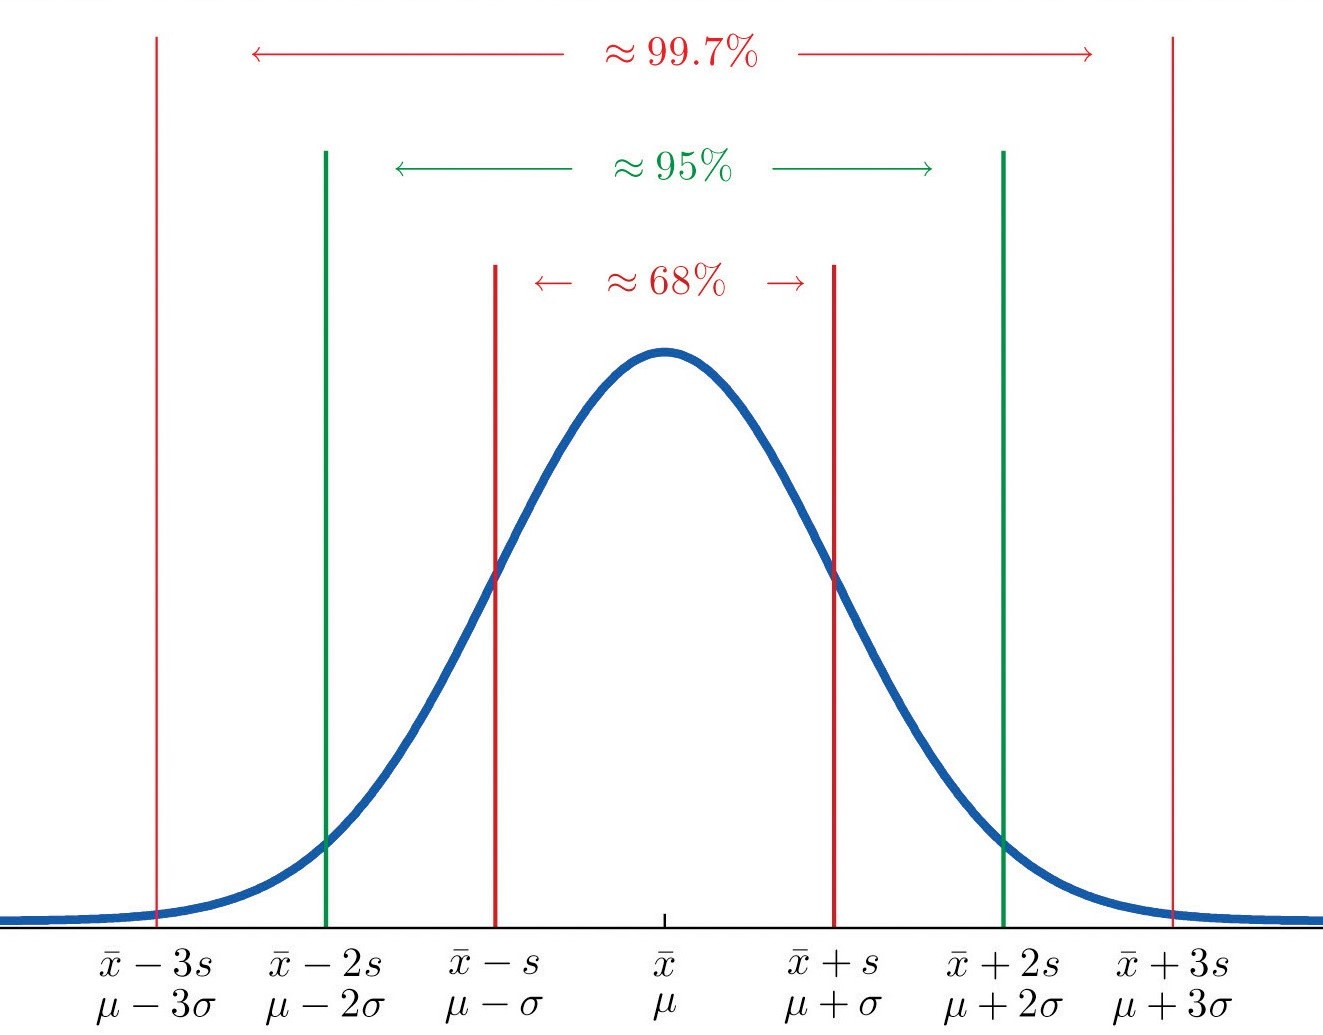
\includegraphics[width=0.9\textwidth]{Figures/Empirical-Rule.jpg}
\end{center}

\hypertarget{chebyshevs-theorem}{%
\subsection{Chebyshev's Theorem}\label{chebyshevs-theorem}}

For any numerical data set, at least \(1-1/k^2\) of the data lie within
\(k\) standard deviations of the mean, where \(k\) is any positive whole
number that is at least 2.
\begin{center}
  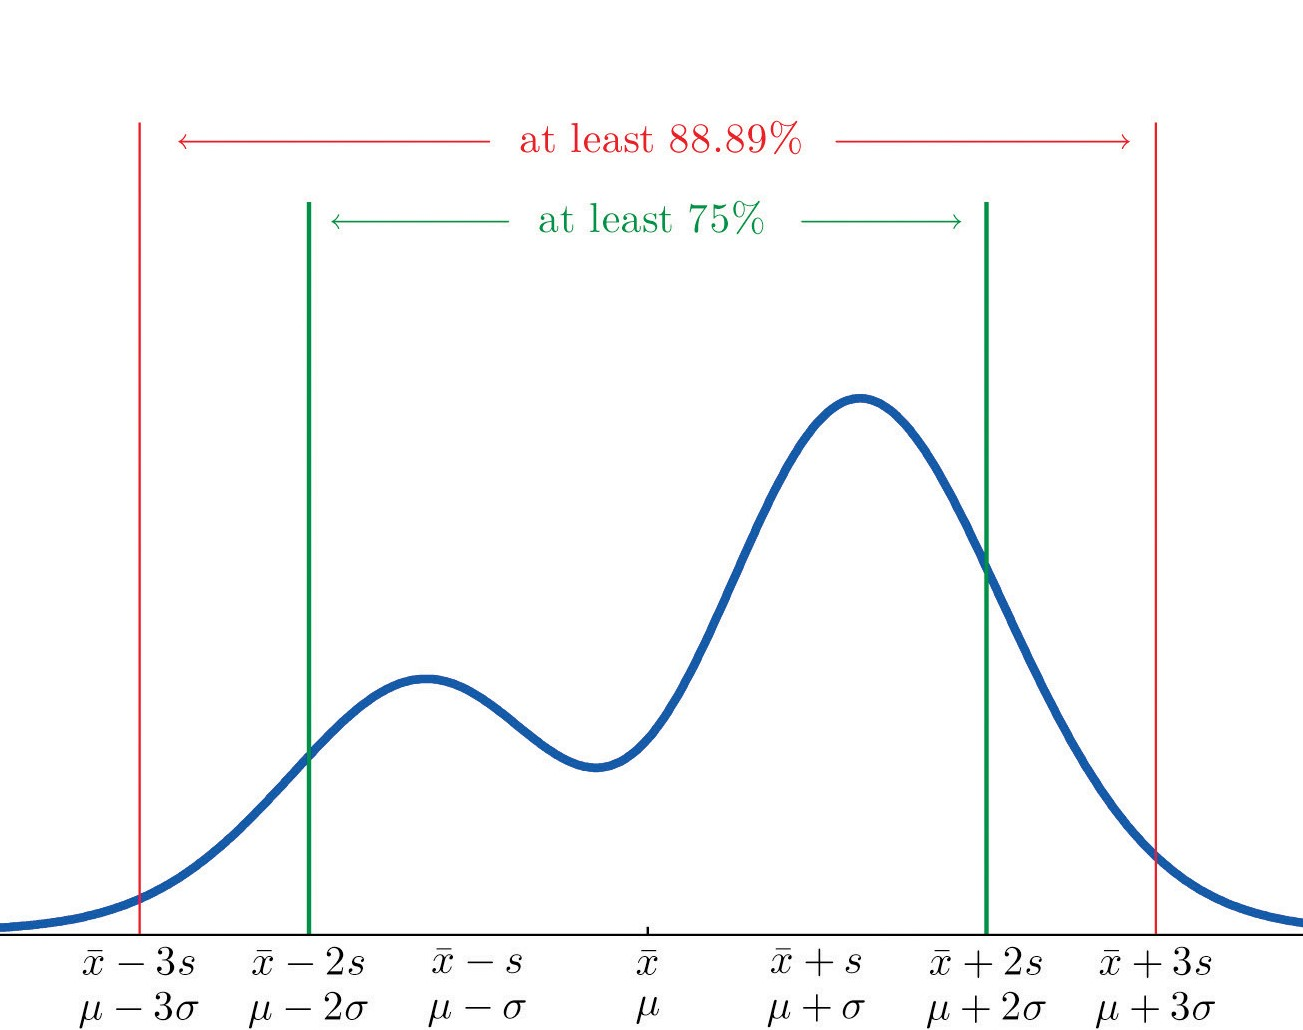
\includegraphics[width=0.9\textwidth]{Figures/Chebyshev.jpg}
\end{center}

\begin{example}

A population data set with a bell-shaped distribution has mean
\(\mu = 6\) and standard deviation \(\sigma = 2\). Find the approximate
proportion of observations in the data set that lie:

\begin{enumerate}
\item
  between 4 and 8;
\item
  below 4.
\end{enumerate}

\end{example}

\begin{example}

A sample data set has mean \(\bar{x}=6\) and standard deviation
\(s = 2\). Find the minimum proportion of observations in the data set
that must lie between 2 and 10.

\end{example}
\vspace*{6\baselineskip}

\begin{exercise}

The maintenance department at the main campus of a large state
university receives daily requests to replace fluorecent lightbulbs. The
distribution of the number of daily requests is bell-shaped and has a
mean of 60 and a standard deviation of 9. Using the 68-95-99.7 rule,
what is the approximate percentage of lightbulb replacement requests
numbering between 60 and 78?

\end{exercise}
\vspace*{6\baselineskip}

\begin{exercise}
  A sample data set has mean \(\bar{x}=10\) and standard deviation
  \(s = 3\). Find the minimum proportion of observations in the data set
  that must lie between 1 and 19.
\end{exercise}
\vspace*{6\baselineskip}

\hypertarget{more-practice}{%
\subsection{More Practice}\label{more-practice}}

\begin{exercise}

A teacher decide to curve the final exam by adding 10 points for each
student. Which of the following statistic will NOT change:
\begin{enumerate*}
  \item median, \item mean, \item interquartile range, \item standard deviation?
\end{enumerate*}
\textbf{Please explain your conclusion.}

\end{exercise}
\vspace*{6\baselineskip}

\begin{exercise}

Which distribution of data has the SMALLEST standard deviation? Please
explain your conclusion.

\begin{fullwidth}
  \begin{center}
    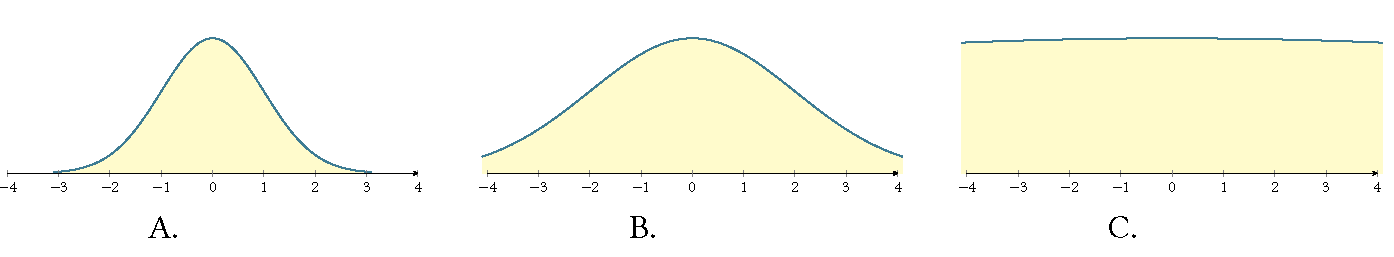
\includegraphics{Figures/SD-Pic.png}
  \end{center}
\end{fullwidth}

\end{exercise}
\vspace*{6\baselineskip}

\hypertarget{lab-3-centers-and-variations}{%
\subsection{Lab 3: Centers and
Variations}\label{lab-3-centers-and-variations}}

\hypertarget{mean-median-quartiles-and-standard-deviation}{%
\subsubsection{Mean, Median, Quartiles and Standard
Deviation}\label{mean-median-quartiles-and-standard-deviation}}

\begin{itemize}
\item
  To find the median, you may use the function \texttt{MEDIAN()}.
\item
  To find quartiles, you may use the function \texttt{QUARTILE.EXC()}.

  \textbf{Note:} this function calculates first and third quartiles with
  25\% and 75\% weights. The results may be different from the results
  calculated by hand discussed in this course.
\item
  To find the mean, you may use the function \texttt{AVERAGE()}.
\item
  To find the \textbf{population} standard deviation, you may use the
  function \texttt{STDEV.P()}.
\item
  To find the \textbf{sample} standard deviation, you may use the
  function \texttt{STDEV.S()}.
\end{itemize}

\hypertarget{how-to-create-a-boxplot-in-excel}{%
\subsubsection{How to Create a Boxplot in
Excel}\label{how-to-create-a-boxplot-in-excel}}

\begin{itemize}
\item
  Select your data---either a single data series, or multiple data
  series.
\item
  Click \texttt{Insert} $\rightarrow$ \texttt{Insert\ Statistic\ Chart}
  $\rightarrow$ \texttt{Box\ and\ Whisker} to create a boxplot.
\end{itemize}

For more information, see
\href{https://support.microsoft.com/en-us/office/create-a-box-and-whisker-chart-62f4219f-db4b-4754-aca8-4743f6190f0d}{Create
a box and whisker chart in Excel 365}

\begin{exercise}

Consider the following sample that consists of speeds of 20 cars.

19, 4, 17, 22, 23, 8, 20, 19, 10, 10, 13, 13, 15, 12, 20, 14, 9, 20, 12,
11

\begin{enumerate}[sepno]
\item
  Use Excel to find the mean, median, quartiles and standard deviation
  of the sample.
\item
  Create a box-plot for the sample.
\end{enumerate}

\end{exercise}


\newlecture

% !TeX root = main.tex

\hypertarget{linear-relationship}{%
\section{Linear Relationship}\label{linear-relationship}}

\hypertarget{scatterplots}{%
\subsection{Scatterplots}\label{scatterplots}}

\begin{itemize}
\item
  Correlation refers to a relationship between two quantitative
  variables:

  \begin{itemize}
  \item
    the independent (or explanatory) variable, usually denoted by \(x\).
  \item
    the dependent (or response) variable, usually denoted by \(y\).
  \end{itemize}
\item
  To describe the relationship between two quantitative variables,
  statisticians use a scatterplot.
\item
  In a scatterplot, we describe the overall pattern with descriptions of
  direction, form, and strength.
\item
  \textbf{Positive relationship}: the response variable (y) increases
  when the explanatory variable (x) increases.

    \item
  \textbf{Negative relationship}: the response variable (y) decreases
  when the explanatory variable (x) increases.

\end{itemize}
\marginpar{
  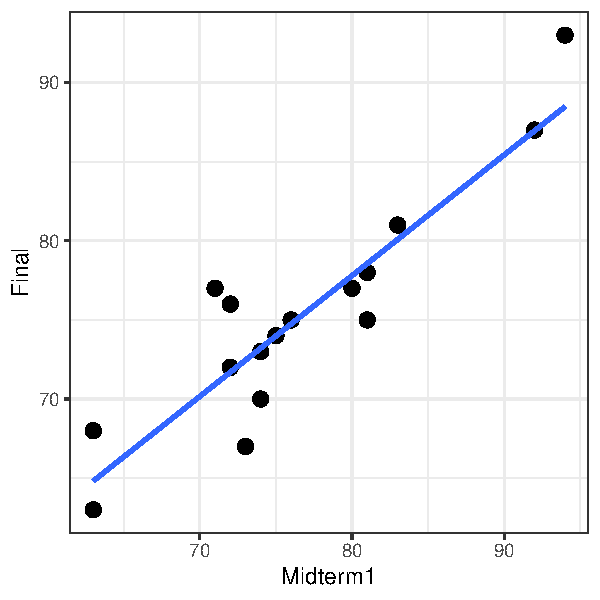
\includegraphics[scale=0.3]{figure-latex/unnamed-chunk-4-2-1}

  \textbf{Positive Relation}

  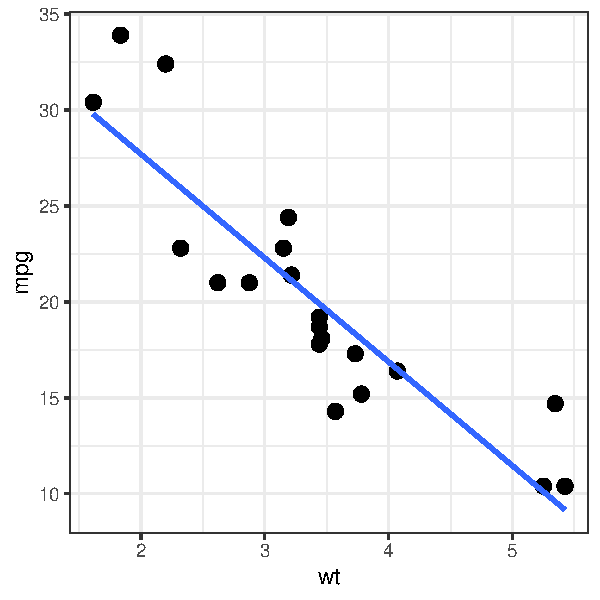
\includegraphics[scale=0.3]{figure-latex/unnamed-chunk-4-3-1}

  \textbf{Negative Relation}
  }

\begin{itemize}
  \item \textbf{Forms of relationship:}
\end{itemize}
\begin{minipage}{1.2\textwidth}
    \begin{minipage}[t]{0.3\textwidth}
      \begin{figure}[H]
        \begin{center}
          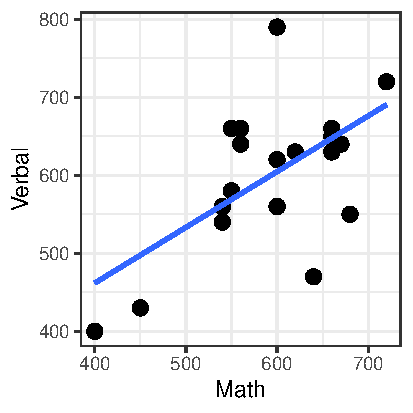
\includegraphics[scale=0.4]{figure-latex/unnamed-chunk-4-4-1}
          
          \textbf{Linear form}
        \end{center}
      \end{figure}
    \end{minipage}
    \begin{minipage}[t]{0.3\textwidth}
      \begin{figure}[H]
        \begin{center}
          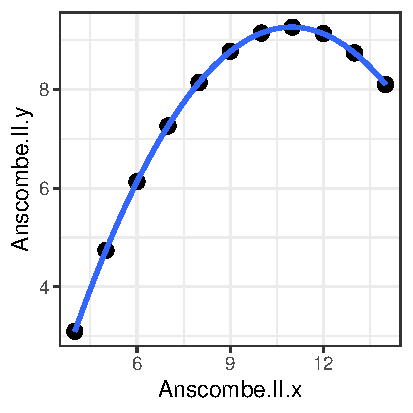
\includegraphics[scale=0.4]{figure-latex/unnamed-chunk-4-5-1}
          
          \textbf{Curvilinear form}
        \end{center}
      \end{figure}
    \end{minipage}
    \begin{minipage}[t]{0.3\textwidth}
      \begin{figure}[H]
        \begin{center}
          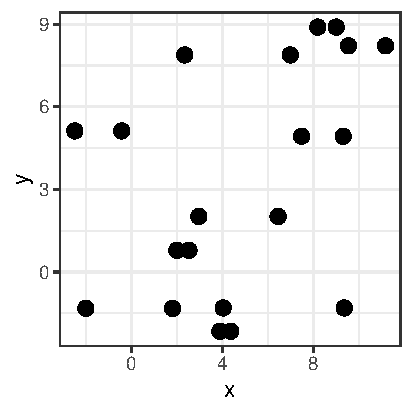
\includegraphics[scale=0.4]{figure-latex/unnamed-chunk-4-6-1}
          
          \textbf{No obvious relationship}
        \end{center}
      \end{figure}
    \end{minipage}
\end{minipage}

\begin{itemize}
\item
  The strength of the relationship is a description of how closely the
  data follow the form of the relationship.

  \begin{center}
    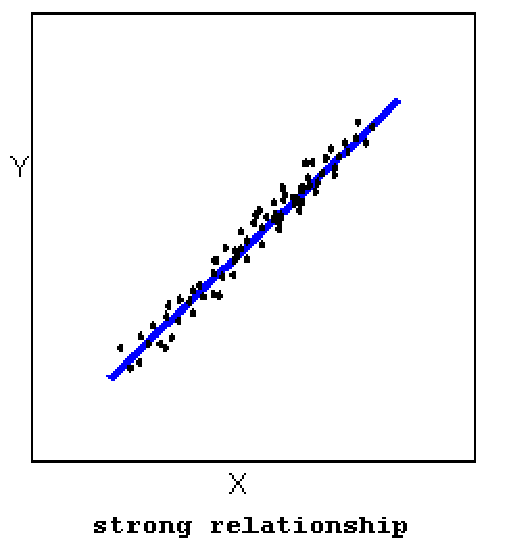
\includegraphics[scale=0.4]{Figures/strong-relation}
    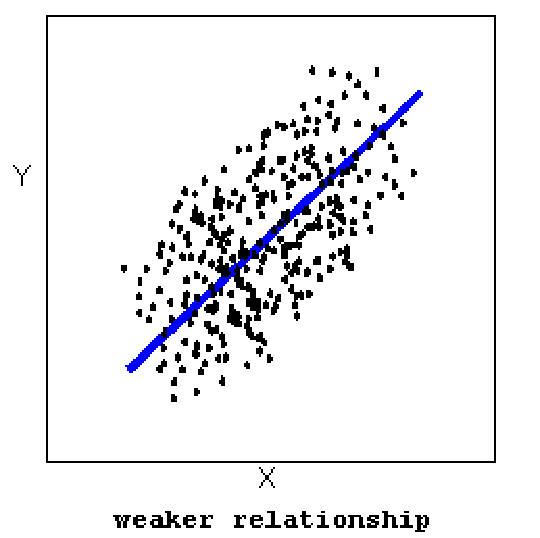
\includegraphics[scale=0.4]{Figures/weaker-relationship}
  \end{center}
\item
  Outliers are points that deviate from the pattern of the relationship.
\begin{center}
  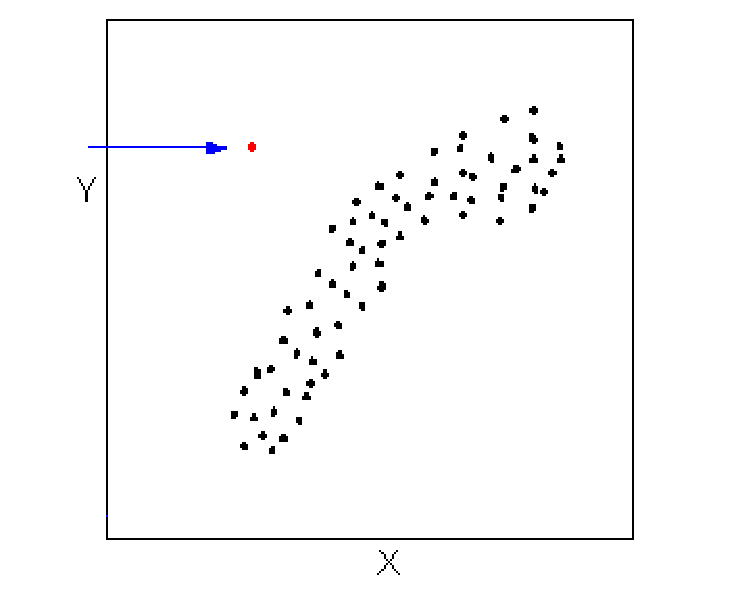
\includegraphics[scale=0.4]{Figures/outlier-in-relationship}
\end{center}
\end{itemize}

\begin{exercise}
Match scatterplots with the descriptions of relations between given variables.

\begin{center}
  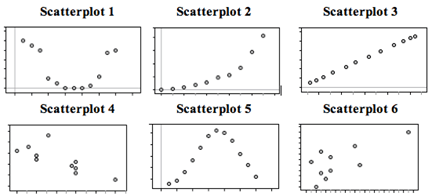
\includegraphics[width=0.8\textwidth]{Figures/MatchScatterplots.png}
\end{center}

\begin{enumerate}[sepno, label={\textbf{\Alph* :}}]
\item X = month (January = 1), Y = rainfall (inches) in Napa, CA
in 2010 (Note: Napa has rain in the winter months and months with little
to no rainfall in summer.)

\item X = month (January = 1), Y = average temperature in Boston
MA in 2010 (Note: Boston has cold winters and hot summers.)

\item X = year (in five-year increments from 1970),
Y = Medicare costs (in \$) (Note: the yearly increase in Medicare costs
has gotten bigger and bigger over time.)

\item X = average temperature in Boston MA (°F), Y = average
temperature in Boston MA (°C) each month in 2010

\item X = chest girth (cm), Y = shoulder girth (cm) for a sample
of men

\item X = engine displacement (liters), Y = city miles per gallon
for a sample of cars (Note: engine displacement is roughly a measure of
engine size. Large engines use more gas.)
\end{enumerate}

\end{exercise}

\hypertarget{the-correlation-coefficient}{%
\subsection{The Correlation
Coefficient}\label{the-correlation-coefficient}}

\begin{itemize}
\item
  The correlation coefficient \(r\) is a numeric measure that measures
  the strength and direction of a linear relationship between two
  quantitative variables. \[
  r=\dfrac{\sum\left(\frac{x-\bar{x}}{s_x}\right)\left(\frac{y-\bar{y}}{s_y}\right)}{n-1},
  \] where \(n\) is the sample size, \(x\) is a data value for the
  explanatory variable, \(\bar{x}\) is the mean of the \(x\)-values,
  \(s_x\) is the standard deviation of the \(x\)-values, and similarly,
  for the notations involving $y$.
\item
  The expression \(z=\frac{x-\bar{x}}{s_x}\) is known as the
  standardized variable (or \(z\)-score) which

  \begin{itemize}
  \item
    doesn't depend on the unit of the variable \(x\),
  \item
    has mean \(0\) and standard deviation 1.
  \end{itemize}
\item
  In Excel, the correlation coefficient can be calculated using the
  function \textsf{CORREL()}.
% \item
%   \href{https://courses.lumenlearning.com/wmopen-concepts-statistics/chapter/linear-relationships-2-of-4/}{Scatterplots
%   with different correlation coefficients}
\item
  \textbf{Rounding Rule:} Round to the nearest thousandth for \(r\),
  \(m\) and \(b\).
\item
  Geometric explanation of the definition of \(r\).
\end{itemize}

\begin{fullwidth}
  \colorbox{white}{
    \parbox{\linewidth}{
  \begin{multicols*}{2}
    \begin{center}
      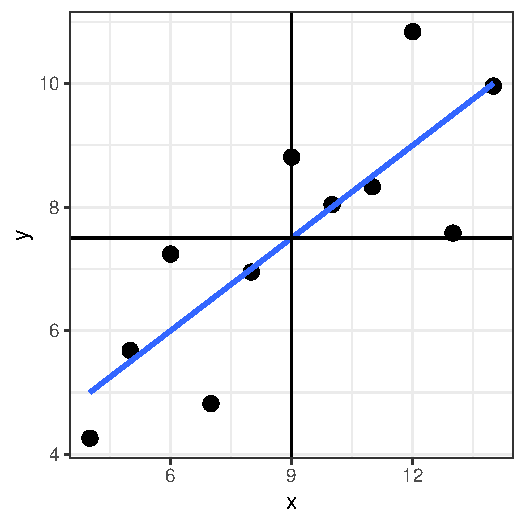
\includegraphics[width=0.6\linewidth]{figure-latex/unnamed-chunk-4-7-1}\\
      $r= 0.816$
    \end{center}

  \columnbreak

  \begin{center}
    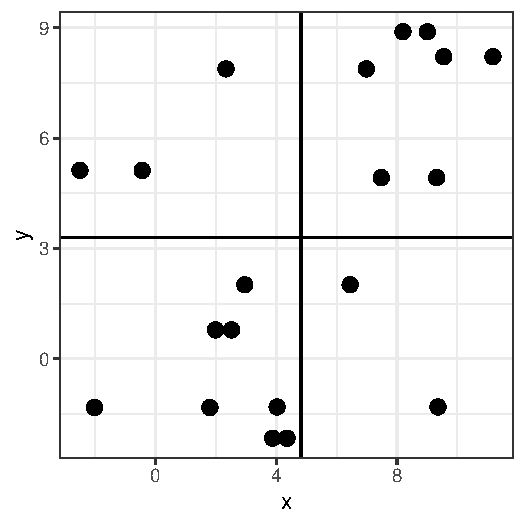
\includegraphics[width=0.6\linewidth]{figure-latex/unnamed-chunk-4-8-1}\\
    \(r=0.420\)
  \end{center}
\end{multicols*}
    }}
\end{fullwidth}


% \begin{remark}

% \begin{itemize}
% \item
%   \(r>0\) if all points \((x-\bar{x}, y-\bar{y})\) are in the 1st and
%   the 3rd quadrants.
% \item
%   \(r<0\) if all points \((x-\bar{x}, y-\bar{y})\) are in the 2nd and
%   the 4th quadrants.
% \end{itemize}

% \end{remark}

\begin{itemize}
\item
  The correlation coefficient \(r\) is between \(-1\) and \(1\).
\item
  The closer the absolute value \(|r|\) is to \(1\), the stronger the
  linear relationship is.
\item
  The correlation is symmetric in \(x\) and \(y\), that is
  \textsf{CORREL(x,\ y)=CORREL(y,\ x)}.
\item
  The correlation does not change when the units of measurement of
  either one of the variables change. In other words, if we change the
  units of measurement of the explanatory variable and/or the response
  variable, it has no effect on the correlation (r).
\item
  The correlation by itself is not enough to determine whether a
  relationship is linear. It's important to graph data set before
  analyzing it.\\
  \href{https://en.wikipedia.org/wiki/Anscombe\%27s_quartet}{https://en.wikipedia.org/wiki/Anscombe\%27s\_quartet}
\item
  The correlation is heavily influenced by outliers.
  \href{https://courses.lumenlearning.com/wmopen-concepts-statistics/chapter/linear-relationships-4-of-4/}{Try
  the simulation in Linear Relation (4 of 4) in Concepts in Statistics}
\item
  The reason that \(|r|\) is less than \(1\) is from the
  \href{https://en.wikipedia.org/wiki/Cauchy\%E2\%80\%93Schwarz_inequality}{Cauchy-Schwarz
  inequality}: \((\sum XY)^2\le \sum X^2\sum Y^2\).
\end{itemize}

\begin{exercise}

  Open the linked website and try  to guess the correlation coefficient.

\href{https://istats.shinyapps.io/guesscorr/}{https://istats.shinyapps.io/guesscorr/}

\end{exercise}

\begin{example}
  Use the data on Midterm 1 and Final from a sample of 10 students.
  \begin{itemize}
    \item
      Draw a scatter plot for the data table.
    \item
      Is it appropriate to study the relationship using a linear model.
    \item
      Find and interpret the correlation coefficient.
    \end{itemize}
  \begin{table}[h]
        \begin{tabular}[c]{l|l}
          \hline
          \multicolumn{1}{c|}{\textbf{Midterm1}} & 
          \multicolumn{1}{c}{\textbf{Final}} \\
          \hline
          72 & 72\\
          93 & 88\\
          81 & 82\\
          82 & 82\\
          94 & 88\\
          80 & 77\\
          73 & 78\\
          71 & 77\\
          81 & 76\\
          81 & 76\\
          63 & 68\\
          \hline
        \end{tabular}
  \end{table}
\end{example}
\vspace*{\baselineskip}

\begin{exercise}

Use the data shown below to answer the following questions.
\begin{itemize}
  \item
    Draw a scatter plot for the data table.
  \item
    Is it appropriate to study the relationship using a linear model.
  \item
    Find and interpret the correlation coefficient.
  \end{itemize}
  \begin{table}[h]
    \begin{small}
        \begin{tabular}[c]{l|l}
          \hline
          \multicolumn{1}{c|}{\textbf{$x$}} & 
          \multicolumn{1}{c}{\textbf{$y$}} \\
          \hline
          4 & 14.86 \\
          5 & 15.65 \\
          6 & 17.94 \\
          7 & 18.63 \\
          8 & 17.12 \\
          9 & 21.11 \\
          10 & 19.7 \\
          11 & 21.99 \\
          \hline
        \end{tabular}
    \end{small}
  \end{table}
\end{exercise}
\vspace*{2\baselineskip}

\hypertarget{correlation-v.s.-causation}{%
\subsection{Correlation v.s.
Causation}\label{correlation-v.s.-causation}}

\begin{itemize}
\item
  Correlation is described by data from observational study.
  Observational studies cannot prove cause and effect which requires
  controlled study and rigorous inferences.
\item
  Correlation may be used to make a prediction which is probabilistic.
\item
  In a linear relationship, an \(r\)-value that is close to 1 or -1 is
  insufficient to claim that the explanatory variable causes changes in
  the response variable. The correct interpretation is that there is a
  statistical relationship between the variables.
\item
  A \textbf{lurking variable} is a variable that is not measured in the
  study, but affects the interpretation of the relationship between the
  explanatory and response variables.
\end{itemize}

\begin{example}

The scatterplot below shows the relationship between the number of
firefighters sent to fires (x) and the amount of damage caused by fires
(y) in a certain city.
\begin{center}
  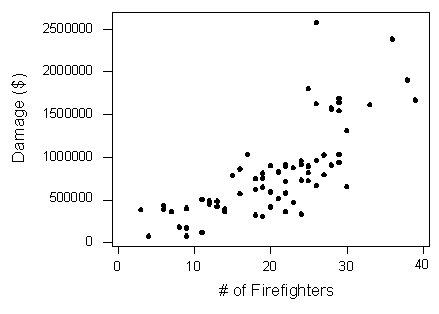
\includegraphics[scale=0.6]{Figures/scatterplot-firefigters.png}
\end{center}

Can we conclude that the increase in firefighters causes the increase in
damage?

\end{example}

\vspace*{2\baselineskip}

\begin{exercise}

Over a period of a few years, the population of Denver increased. It was
observed that during this period the correlation between the number of
people attending church and the number of people receiving traffic
tickets was \(r = 0.92\). Does going to church cause people to get
traffic tickets? Is there a lurking variable that might cause both
variables to increase?

\end{exercise}
\vspace*{2\baselineskip}

\hypertarget{the-regression-line}{%
\subsection{The Regression Line}\label{the-regression-line}}

\begin{itemize}
\item
  The line that best summarizes a linear relationship is \textbf{the
  least squares regression line}. The regression line is the line with
  the smallest sum of squares of the errors (\textbf{SSE}).
\item
  We use the least-squares regression line to predict the value
  \(\hat{y}\) for a value of the explanatory variable \(x\).
\item
  The regression line is unique and passes though
  \((\bar{x}, \bar{y})\). The equation is given by
  \[\hat{y}=m(x-\bar{x})+\bar{y}=m x+b,\] where the slope is
  \[m=\frac{\sum(x-\bar{x})(y-\bar{y})}{\sum(x-\bar{x})^2}=r\frac{s_y}{s_x}\]
  and the \(y\)-intercept is \(b=\bar{y}-m\bar{x}.\)
\item
  The \textbf{error of a prediction} is
  \[\text{Error}=\text{Observed}-\text{Predicted}=y-\hat{y}.\]
\item
  A prediction beyond the range of the data is called
  \textbf{extrapolation}.
\end{itemize}

\begin{example}
  The following sample is taken from data about the Old Faithful geyser.

  \begin{enumerate}[sepno]
    \item
      Study the linear relationship. Is it positive? What's the strength? What's the direction?
    \item
      Find the regression line, and the predicated value and the error if
      the eruption time is 1.8 minutes.
    \end{enumerate}

    \begin{tabular}[c]{l|l}
      \hline
      \multicolumn{1}{c|}{\textbf{eruptions}} & 
      \multicolumn{1}{c}{\textbf{waiting}} \\
      \hline
      3.917 & 84\\
      1.75 & 62\\
      4.200 & 78\\
      4.80 & 84\\
      1.750 & 47\\
      1.60 & 52\\
      4.700 & 83\\
      4.25 & 79\\
      2.167 & 52\\
      1.80 & 51\\
      \hline
    \end{tabular}
\end{example}

\vspace*{3\baselineskip}

\begin{exercise}
Research was conducted on the amount of training for 5K and the time a
contestant took to run the race. The researcher recorded the number of
miles during training ( a 1-month period) and the time to complete the
5K. The results are below.

\begin{longtable}[]{@{}ccccccc@{}}
\toprule()
Miles Trained & 20 & 69 & 102 & 29 & 46 & 68 \\
\midrule()
\endhead
Time(Minutes) & 37.26 & 38.3 & 39.96 & 29.95 & 26.56 & 43.78 \\
\bottomrule()
\end{longtable}
\begin{enumerate}
\item
  Find the correlation coefficient.
\item
  Find the equation of regression line.
\item
  Predict the time in the 5K if someone trained 29 miles.
\item
  Find the residual (the prediction error) for 102 miles trained.
\end{enumerate}

\end{exercise}

\hypertarget{assessing-the-fit-of-a-regression-line}{%
\subsection{Assessing the Fit of a Regression
Line}\label{assessing-the-fit-of-a-regression-line}}

\begin{itemize}
\item
  The prediction error is also called a \textbf{residual}. Another way
  to express the previous equation for error is
  \[y=\hat{y}+\text{residual}.\]
\item
  \textbf{Residual plots} are used to determine if a linear model is
  appropriate.

  A random pattern (or no obvious pattern) indicates a good fit of a
  linear model.
  \href{https://courses.lumenlearning.com/wmopen-concepts-statistics/chapter/assessing-the-fit-of-a-line-2-of-4/}{See
  Assessing the Fit of a Line (2 of 4) in Concepts in Statistics for
  examples.}
\item
  A ``typical'' error used to measure the fit of the regression is the
  \textbf{residual standard errors} (or \textbf{standard error of the
  regression}), calculated by the Excel function \textsf{STEYX()}, is
  \[s_e=\sqrt{\dfrac{SSE}{n-2}},\] where \(SSE=\sum (y-\hat{y})^2\) is
  the sum of square errors.
\item
  The smaller \(s_e\) is, the more accurate the prediction is.
\item
  The fit of a regression line can also be measured by the proportion of
  the variation in the response variable that is explained by the
  least-squares regression line. This proportion is known as the
  \textbf{coefficient of determination}.

  \begin{itemize}
  \item
    The \textbf{total variance} is \(SSD=\sum(y-\bar{y})^2\)
  \item
    The \textbf{explained variance} is \(SSR=\sum(\hat{y}-\bar{y})^2\).
  \item
    The \textbf{coefficient of determination} is
    \[r^2=\dfrac{SSR}{SSD}=\dfrac{\sum(y-\bar{y})^2}{\sum(\hat{y}-\bar{y})^2}.\]
  \end{itemize}
\end{itemize}

\begin{remark}

\begin{itemize}
\item
  The \(r\) in the coefficient of determination is the correlation
  coefficient. Equivalently, \(r=\pm\sqrt{r^2}\).
\item
  The smaller the standard error, the larger the coefficient of
  determination: \[r^2=1-\dfrac{SSE}{SSD}=1-\dfrac{(n-2)s_e^2}{SSD}.\]
\item
  \(n-2\) is the degrees of freedom. We lose two degrees of freedom
  because we estimate the slope and the \(y\)-intercept.
\item
  In a linear regression model \(Y=\beta_0 + \beta_1 X +\epsilon\), even
  we have \(\beta_0\) and \(\beta_1\) from the population, we still need
  estimate the standard deviation of error.
\end{itemize}

\end{remark}

\begin{example}

Find the standard error and coefficient of determination for the data of midterm1 and final.

\begin{table}[h]
      \begin{tabular}[c]{l|*{10}{c}}
        \hline
        \textbf{Midterm1} & 72 & 93 & 81 & 82 & 94 & 80 & 73 & 71 & 81 & 81\\
        \hline
\textbf{Final} & 72 & 88 & 82 & 82 & 88 & 77 & 78 & 77 & 76 & 76\\
        \hline
      \end{tabular}
\end{table}
\end{example}
\vspace*{5\baselineskip}

\begin{exercise}
A researcher measures the wrist circumference and height of a random
sample of individuals. The data are displayed below.

\begin{fullwidth}
  \colorbox{white}{
    \parbox{\linewidth}{
  \begin{center}
    \begin{tabular}[c]{l|*{10}{p{0.055\linewidth}}}
      \hline
        \textbf{Wrist Size (in)} & 5.5 & 5.6 & 5.8 & 5.9 & 6.1 & 6.3 & 6.4 & 6.5 & 6.6 & 6.8\\ 
        \hline
        \textbf{Height (in)} & 60.4 & 59.7 & 66.3 & 63.5 & 60.4 & 66.9 & 65.6 & 70.9 & 59.7 & 64.9 \\
      \hline
    \end{tabular}
  \end{center}
    }}
\end{fullwidth}

\begin{enumerate}
\item
  Find the equation of the best-fit line~\(y=mx+b\).~
\item
  Find the correlation coefficient.
\item
  Predict the height of a person with a wrist circumference of 6 inches
  using the best-fit line.
\item
  Calculate the residual for the point (6.5,70.9).
\item
  When predicting heights, what is a ``typical'' error of this linear
  model?
\item
  What proportion of variability in heights can be explained by this
  linear model? (Write your answer in decimal.)
\item
  Find the correlation coefficient if the heights are measured in feet.
\end{enumerate}

\end{exercise}

\hypertarget{lab-4-linear-regressions}{%
\subsection{Lab 4: Linear Regressions}\label{lab-4-linear-regressions}}

\begin{itemize}
\item
  To create a scatter plot, first select the data sets, and then look
  for \textsf{Insert\ Scatter(X,\ Y)} in the menu
  \textsf{Insert} $\rightarrow$ \textsf{Charts}.
\item
  The correlation coefficient \(r\) can be calculated by the Excel
  function \textsf{correl()}.
\item
  The slope of a linear regression can be calculated by the Excel
  function \textsf{SLOPE()}.
\item
  The \(y\)-intercept of a linear regression can be calculated by the
  Excel function \textsf{INTERCEPT()}.
\item
  The coefficient of determination can be calculated by first finding
  \(r\), then applying the formula \textsf{r\^{}2}.
\item
  The standard error of the regression (residual standard error) can be
  calculated by the Excel function \textsf{STEYX()}.
\end{itemize}

\begin{exercise}
  A researcher measures the wrist circumference and height of a random sample of individuals. The data and the scatterplot are displayed below.

  \begin{fullwidth}
    \colorbox{white}{
    \parbox{\linewidth}{
    \begin{center}
      \begin{tabular}[c]{l|*{12}{p{0.0375\linewidth}}}
      \hline  
      \textbf{Wrist Size (in)} &	5.7 & 5.9 & 6 & 6.2 & 6.3 & 6.5 & 6.7 & 7.1 & 7.3 & 8 & 8.2 & 8.4\\
      \hline
      \textbf{Height (in)} & 62.8 & 68.3 & 68.7 & 59.1 & 61.2 & 67.6 & 69.7 & 70.6 & 75.2 & 80.8 & 78.2 & 80.9\\
      \hline
      \end{tabular}
    \end{center}
    }}
  \end{fullwidth}

\begin{enumerate}
  \item Create a scatterplot for the data.
  \item Find the equation of the best-fit line $y=mx+b$.
  \item Predict the height of a person with a wrist circumference of 6 inches using the best-fit line. 
  \item Calculate the residual for the point (5.9,68.3). 
  \item When predicting heights, what is a "typical" error of this linear model? 
 \item What proportion of variability in heights can be explained by this linear model?
  \item Find the correlation coefficient if the heights are measured in feet. 
\end{enumerate}
\end{exercise}
\newlecture

% !TeX root = main.tex

\section{Two-way Tables}

\hypertarget{two-way-frequency-tables}{%
\subsection{Two-way Frequency Tables}\label{two-way-frequency-tables}}

\begin{itemize}
\item
  As we organize and analyze data from two categorical variables, we
  make use of two-way tables.
\item
  Information in a \textbf{two-way frequency table}:

  \begin{itemize}
  \item
    Values of the two variables are displayed in the left column and the
    top row.
  \item
    The body of table consists of frequency counts associated to pairs
    of values of the two variables.
  \item
    The right column and the bottom row, which are called margins of the
    table, consists of row totals and column totals respectively.
  \end{itemize}
\item
  A number in a margin are called \textbf{marginal frequency}.
\item
  A numbers in the body of the table is called \textbf{joint frequency}.
\end{itemize}

\begin{example}

The following table summarize responses of a random sample of 1,200 U.S.
college students as part of a larger survey.

\begin{fullwidth}
  \colorbox{white}{
    \parbox{\linewidth}{\centering
  \begin{tabular*}{0.8\linewidth}{l*{4}{m{0.15\linewidth}}}
  \toprule
   & About Right
  & Overweight
  & Underweight
  & Row Totals\\
  \midrule
  Female & 560 & 163 & 37 & 760 \\
  Male & 295 & 72 & 73 & 440 \\
  Column Totals & 855 & 235 & 110 & 1,200 \\
  \bottomrule
  \end{tabular*}
  }}
\end{fullwidth}

\end{example}

\hypertarget{two-way-relative-frequency-tables-and-probability}{%
\subsection{Two-Way Relative Frequency Tables and
Probability}\label{two-way-relative-frequency-tables-and-probability}}

\begin{itemize}
\item
  A \textbf{two-way relative frequency table} is obtained from a two-way
  frequency table by converting frequencies in a two-way table to
  relative frequencies.
\item
  \textbf{Marginal probability}
  \[P(X)=\frac{\text{Marginal frequency in}~ X}{\text{Total}}\]
\item
  \textbf{Conditional probability}
  \[P(X|Y)=\frac{\text{Joint frequency}}{\text{Marginal Frequency in}~Y}\]
  \[P(Y|X)=\frac{\text{Joint frequency}}{\text{Marginal Frequency in}~X}\]
\item
  \textbf{Joint probability}
  \[P(X\text{and}~ Y)=\frac{\text{Joint frequency}}{\text{Total}}\]
\item
  Note that \(P(X~\text{and}~Y)=P(X)\cdot P(Y|X)=P(Y)\cdot P(X|Y).\)
\end{itemize}

\begin{example}

The following table shows joint and marginal probabilities of body image
and gender.

\begin{fullwidth}
  \colorbox{white}{
    \parbox{\linewidth}{\centering
  \begin{tabular*}{0.9\linewidth}{l*{4}{p{0.15\linewidth}}}
  \toprule
  & About Right
  & Overweight
  & Underweight
  & Row Totals\\
  \midrule
  Female & \(\frac{560}{1200}=46.67\%\) &
  \(\frac{163}{1200}=13.58\%\) & \(\frac{37}{1200}=3.08\%\) &
  \(\frac{760}{1200}=63.33\%\) \\
  Male & \(\frac{295}{1200}=24.58\%\) & \(\frac{72}{1200}=6.00\%\) &
  \(\frac{73}{1200}=6.08\%\) & \(\frac{440}{1200}=36.67\%\) \\
  Column Totals & \(\frac{855}{1200}=71.25\%\) &
  \(\frac{235}{1200}=19.58\%\) & \(\frac{110}{1200}=9.17\%\) &
  \(\frac{1200}{1200}=100.00\%\) \\
  \bottomrule
  \end{tabular*}
}}
\end{fullwidth}

\end{example}

\begin{example}

The following table shows probabilities of randomly select male or
female who has a certain body image.

\begin{fullwidth}
  \colorbox{white}{
    \parbox{\linewidth}{\centering
  \begin{tabular*}{0.8\linewidth}{l*{4}{m{0.15\linewidth}}}
  \toprule
  & About Right
  & Overweight
  & Underweight
  & Row Totals\\
  \midrule
  Female & \(\frac{560}{760}=73.68\%\) & \(\frac{163}{760}=21.45\%\)
  & \(\frac{37}{760}=4.87\%\) & \(\frac{760}{760}=100.00\%\) \\
  Male & \(\frac{295}{440}=67.05\%\) & \(\frac{72}{440}=16.36\%\) &
  \(\frac{73}{440}=16.59\%\) & \(\frac{440}{440}=100.00\%\) \\
  \bottomrule
  \end{tabular*}
}}
\end{fullwidth}

\end{example}

\begin{example}

The following table summarizes the full-time enrollment at a community
college.

\begin{fullwidth}
  \colorbox{white}{
    \parbox{\linewidth}{
      \centering
      \begin{tabular*}{0.9\linewidth}{l*{7}{m{0.08\linewidth}}}
        \hline
        & Arts-Sci
        & Bus-Econ
        & Info Tech
        & Health Science
        & Graphics Design
        & Culinary Arts
        & Row Totals\\
        \hline
        Female & 4,660 & 435 & 494 & 421 & 105 & 83 & 6,198 \\
        Male & 4,334 & 490 & 564 & 223 & 97 & 94 & 5,802 \\
        Column Totals & 8,994 & 925 & 1,058 & 644 & 202 & 177 & 12,000 \\
      \hline
      \end{tabular*}
  }}
\end{fullwidth}

\begin{enumerate}
\item
  What proportion of the total number of students are male students?\\
\item
  If we select a male student at random, what is the probability that he
  is in the Info Tech program?\\
\item
  If a student is selected at random, what is the probability that the
  student is a male and in the Info Tech program?\\
\item
  How are those three probabilities related?
\end{enumerate}

\end{example}

\begin{exercise}

This table relates the weights and heights of a group of individuals
participating in an observational study.\\
\begin{longtable}[]{@{}
  >{\centering\arraybackslash}p{(\columnwidth - 6\tabcolsep) * \real{0.2500}}
  >{\centering\arraybackslash}p{(\columnwidth - 6\tabcolsep) * \real{0.2500}}
  >{\centering\arraybackslash}p{(\columnwidth - 6\tabcolsep) * \real{0.2500}}
  >{\centering\arraybackslash}p{(\columnwidth - 6\tabcolsep) * \real{0.2500}}@{}}
\toprule()
\begin{minipage}[b]{\linewidth}\centering
~Weight/Height~
\end{minipage} & \begin{minipage}[b]{\linewidth}\centering
~Tall~
\end{minipage} & \begin{minipage}[b]{\linewidth}\centering
~Medium~
\end{minipage} & \begin{minipage}[b]{\linewidth}\centering
~Short~
\end{minipage} \\
\midrule()
\endhead
Obese & 18 & 28 & 14 \\
Normal & 20 & 51 & 28 \\
Underweight & 12 & 25 & 9 \\
\bottomrule()
\end{longtable}

\begin{enumerate}
\item
  Find the total for each row and column
\item
  Find the probability that a randomly chosen individual from this group
  is Short.
\item
  Find the probability that a randomly chosen individual from this group
  is Obese and Short.
\item
  Find the probability that a randomly chosen individual from this group
  is Underweight given that the individual is Tall.
\end{enumerate}

\end{exercise}


\hypertarget{test-of-no-association}{%
\subsection{Test of (No) Association}\label{test-of-no-association}}

\begin{itemize}
\item
  To understand association between categorical variables, we may think
  conversely. How do we test no association?
\item
  If the conditional probabilities are nearly equal for all categories,
  there may be no association between the variables. Conversely, if the
  conditional probabilities are different enough, we are confidence to
  say there is an association.
\item
  In general, the bigger the differences in the conditional
  probabilities, the stronger the association between the variables.
\item
  Two variables \(X\) and \(Y\) are \textbf{independent} if
  \(P(X~\text{and}~Y)=P(X)\cdot P(Y)\). Equivalently, \(P(X|Y)=P(X)\)
  and \(P(Y|X)=P(Y)\).
\end{itemize}

\begin{example}

Is body image related to gender?

\begin{fullwidth}
  \colorbox{white}{
    \parbox{\linewidth}{
\centering
\begin{tabular}[c]{*{5}{l}}
  \hline
  \multicolumn{1}{c}{\textbf{}} & 
  \multicolumn{1}{c}{\textbf{About Right}} & 
  \multicolumn{1}{c}{\textbf{Overweight}} &
  \multicolumn{1}{c}{\textbf{Underweight}} &
  \multicolumn{1}{c}{\textbf{Row Totals}} \\
  \hline
  Female & 560 &
163 & 37 & 760 \\
Male &
295 & 72 & 73 & 440 \\
Column Totals & 855 & 235 & 110 &
1,200\\       
  \hline
\end{tabular}

  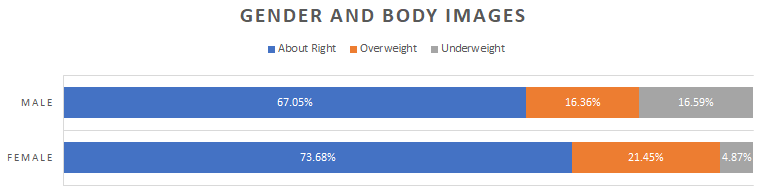
\includegraphics[width=0.9\linewidth]{Figures/Gender-Body.png}
  }}
\end{fullwidth}

\end{example}
\vspace*{\baselineskip}

\hypertarget{percentage-reduction-of-risk}{%
\subsection{Percentage Reduction of
Risk}\label{percentage-reduction-of-risk}}

\begin{itemize}
\item
  When calculating the probability of a negative outcome, we often refer
  to the probability as a \textbf{risk}.
\item
  In general, we are interested in determining how much a new treatment
  reduces the risk compared to a reference risk
\item
  The \textbf{percentage reduction of risk} is
\begin{fullwidth}
  \begin{flushright}
    \colorbox{white}{
    $\text{percentage reduction of risk}=\dfrac{\text{new treatment risk}-\text{reference risk}}{\text{reference risk}}.$
  } 
  \end{flushright}
\end{fullwidth}
\end{itemize}

\begin{example}

Researchers in the Physicians' Health Study (1989) designed a randomized
double-blind experiment to determine whether aspirin reduces the risk of
heart attack. Here are the final results.

\begin{longtable}[]{@{}
  >{\centering\arraybackslash}p{(\columnwidth - 6\tabcolsep) * \real{0.2209}}
  >{\centering\arraybackslash}p{(\columnwidth - 6\tabcolsep) * \real{0.2791}}
  >{\centering\arraybackslash}p{(\columnwidth - 6\tabcolsep) * \real{0.3140}}
  >{\centering\arraybackslash}p{(\columnwidth - 6\tabcolsep) * \real{0.1860}}@{}}
\toprule()
\begin{minipage}[b]{\linewidth}\centering
\end{minipage} & \begin{minipage}[b]{\linewidth}\centering
\textbf{Heart Attack}
\end{minipage} & \begin{minipage}[b]{\linewidth}\centering
\textbf{No Heart Attack}
\end{minipage} & \begin{minipage}[b]{\linewidth}\centering
\textbf{Row Totals}
\end{minipage} \\
\midrule()
\endhead
\textbf{Aspirin} & 139 & 10,898 & 11,037 \\
\textbf{Placebo} & 239 & 10,795 & 11,034 \\
\textbf{Column Totals} & 378 & 21,693 & 22,071 \\
\bottomrule()
\end{longtable}

\emph{Does aspirin lower the risk of having a heart attack?}

\end{example}
\vspace*{6\baselineskip}

\hypertarget{hypothetical-two-way-tables}{%
\subsection{Hypothetical Two-way
Tables}\label{hypothetical-two-way-tables}}

A \textbf{hypothetical two-way table}, also known as a hypothetical 1000
two-way table, is a two-way table constructed from given probability
conditions with 1000 or higher as the total frequency. It can be used to answer
complex probability questions.

\begin{example}

A pregnant woman often opts to have an ultrasound to predict the gender
of her baby. Assume the following facts are known:

\begin{itemize}
\item
  Fact 1: 48\% of the babies born are female.
\item
  Fact 2: 90\% of girls were correctly identified.
\item
  Fact 3: 75\% of boys were correctly identified.
\end{itemize}

Use the above facts to answer the following questions.

\begin{enumerate}
\item
  If the examination predicts a girl, how likely the baby will be a
  girl?
\item
  If the examination predicts a boy, how likely the baby will be a boy?
\end{enumerate}

\end{example}

\begin{exercise}

The table below is based on a 1988 study of accident records conducted
by the Florida State Department of Highway Safety. 

\begin{tabular}{*{4}{l}}
  \hline
  &\textbf{Nonfatal}~ &\textbf{Fatal}~
    &\textbf{Row Totals}~  \\
    \hline
    \textbf{Seat Belt}
  & 412,368 & 510 & 412,878\\
  \textbf{No Seat Belt} & 162,527 & 1,601
  & 164,128\\
  \textbf{Column Totals}
  & 574,895 & 2,111 & 577,006\\
  \hline
\end{tabular}

\emph{Does wearing a seat belt lower the risk of an accident resulting
in a fatality?}

\end{exercise}
\vspace*{6\baselineskip}

\begin{exercise}

A large company has instituted a mandatory employee drug screening
program. Assume that the drug test used is known to be 99\% accurate.
That is, if an employee is a drug user, the test will come back positive
(``drug detected'') 99\% of the time. If an employee is a non-drug user,
then the test will come back negative (``no drug detected'') 99\% of the
time. Assume that 2\% of the employees of the company are drug users.

If an employee's drug test comes back positive, what is the probability
that the test is wrong and the employee is in fact a non drug user?

\end{exercise}
\vspace*{6\baselineskip}

\hypertarget{create-stacked-bar-chart-in-excel}{%
\subsection{Create Stacked Bar Chart in
Excel}\label{create-stacked-bar-chart-in-excel}}

To create a a stacked bar chart of a two-way table

\begin{itemize}
\item
  First select the data table.
\item
  Look for and click \texttt{Insert\ Column\ or\ Bar\ Chart} in the
  menu \texttt{Insert} $\rightarrow$ \texttt{Charts}.
\item
  In the dropdown menu, choose the third option in 2-D Column
  (\texttt{100\%\ Stacked\ Column}) or the third option 2-D Bar
  (\texttt{100\%\ Stacked\ Bar}).
\item
  To switch row/column, in the output graph, right click the row axis
  or the column axis, and chose the option \texttt{Select\ Data...} to
  make a switch.
\end{itemize}
\begin{exercise}

The following table summarize results from a study on program selection
and gender.\\
\begin{fullwidth}
  \colorbox{white}{
    \parbox{\linewidth}{\centering
  \begin{tabular*}{0.9\linewidth}{l*{7}{p{0.08\linewidth}}}
  \toprule
  & Arts-Sci
  & Bus-Econ
  & Info Tech
  & Health Science
  & Graphics Design
  & Culinary Arts
  & Row Totals
  \\
  \midrule
  Female & 4,660 & 435 & 494 & 421 & 105 & 83 & 6,198 \\
  Male & 4,334 & 490 & 564 & 223 & 97 & 94 & 5,802 \\
  Column Totals & 8,994 & 925 & 1,058 & 644 & 202 & 177 & 12,000 \\
  \bottomrule
  \end{tabular*}
  }}
\end{fullwidth}

Use Excel to answer the following question about the study.

\begin{enumerate}
\item
  Is there an association between gender and program selection? Why or
  why not?
\item
  If they are associated, is the association strong or week?
\end{enumerate}

\end{exercise}


\newlecture

% !TeX root = main.tex

\section{Basics of Probability}

\hypertarget{experiments-sample-spaces-and-events}{%
\subsection{Experiments, Sample Spaces, and
Events}\label{experiments-sample-spaces-and-events}}

\begin{itemize}
\item
  An \textbf{experiment} is a procedure that can be infinitely repeated
  and has a well-defined set of outcomes.
\item
  An \textbf{outcome} is the result of a single trial (individual
  repetition) of an experiment.
\item
  A \textbf{chance experiment} (or \textbf{random experiment}) is an
  experiment that has more than one possible outcome and whose outcomes
  cannot be predicted with certainty.
\item
  The \textbf{sample space} of a chance experiment is the set of all
  possible outcomes.
\item
  An \textbf{event} is a subset of the sample space.
\end{itemize}

\begin{example}
A classic example of chance experiment is to toss a fair coin. The following figure shows observed outcomes from an experiment of tossing a coin 100 times as well as the true probabilities of getting a head and a tail.\\ (See \url{https://seeing-theory.brown.edu})

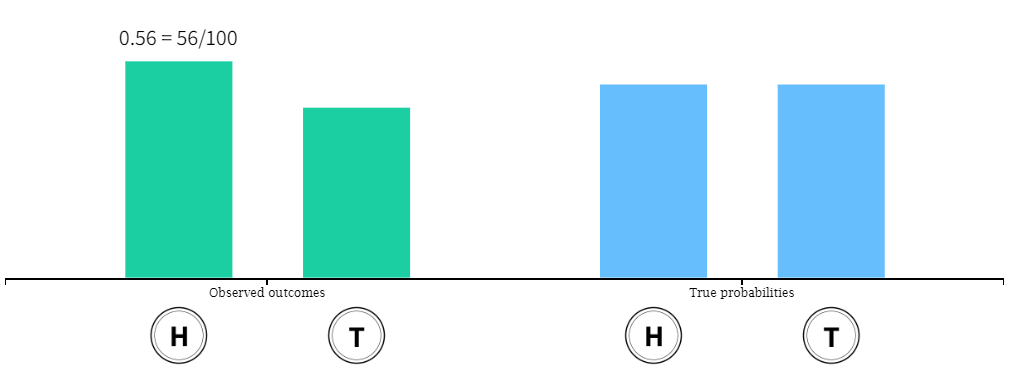
\includegraphics[width=\textwidth]{Figures/ChanceEvent.png}


\end{example}

\hypertarget{complement-intersection-and-union}{%
\subsection{Complement, Intersection and
Union}\label{complement-intersection-and-union}}

\begin{itemize}
\item
  The \textbf{complement} \(E^c\) of event \(E\) is the set of all
  outcomes in a sample space that are \textbf{NOT} included in event
  \(E\).
\item
  The \textbf{intersection} \(A\cap B\) of two events \(A\) and \(B\) is
  the set of all outcomes in the sample space that are shared by \(A\)
  and \(B\).
\item
  The \textbf{union} \(A\cup B\) of two events \(A\) and \(B\) is the
  set of all outcomes in the sample space that are either in \(A\) or
  \(B\).
\item
  Two events \(A\) and \(B\) are \textbf{mutually exclusive} if there
  intersection \(A\cap B\) is empty.
\end{itemize}

% \begin{fullwidth}
  \begin{center}
    \textbf{Venn Diagrams for Complement, Intersection, and Union}\\
    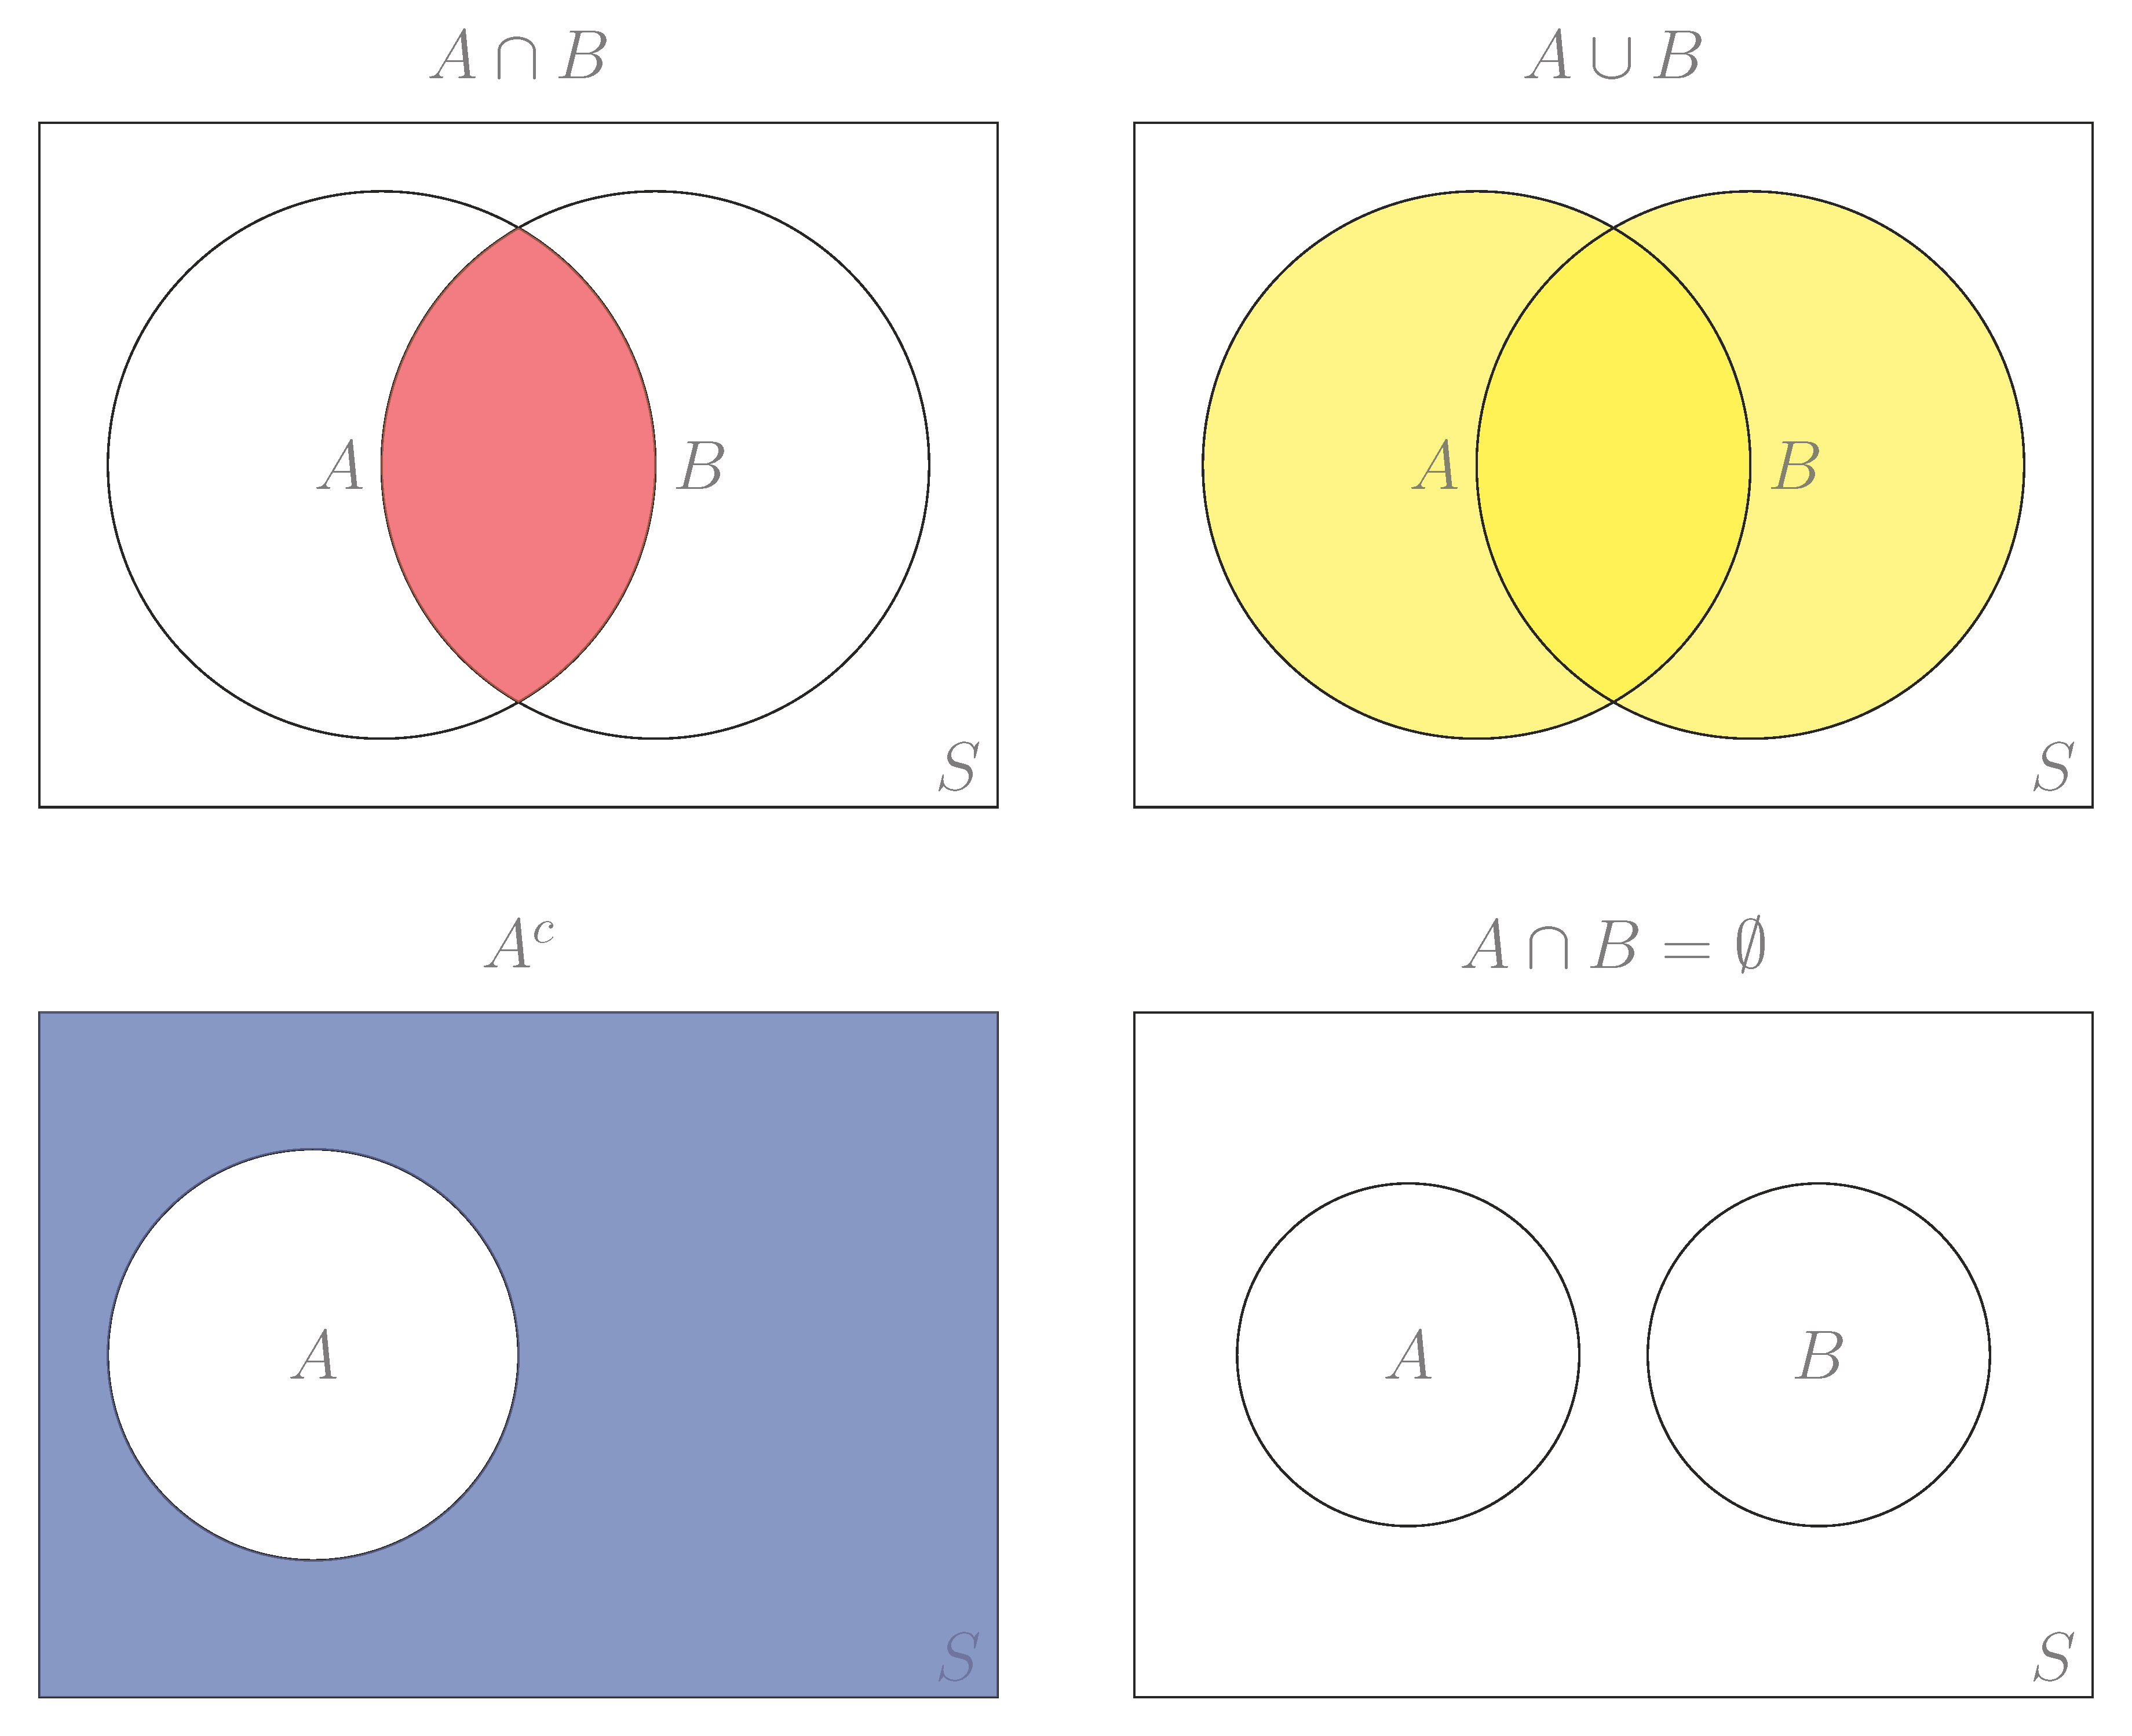
\includegraphics[scale=0.6]{Figures/VennDiagrams.png}
  \end{center}
% \end{fullwidth}

\hypertarget{classical-definition-of-probability}{%
\subsection{Classical Definition of
Probability}\label{classical-definition-of-probability}}

\begin{itemize}
\item
  A \textbf{probability} \(P(E)\) is the measures of how likely an
  outcome in the event \(E\) will occur in a chance experiment.
\item
  \textbf{Equally likely} means that each outcome of an experiment
  occurs with equal chance.
\item
  When the outcomes in the sample space of an chance experiment are
  \textbf{\emph{equally likely}}, the probability of an event \(E\) is
  \[P(E)=\dfrac{\text{number of outcomes in }E}{\text{number of outcomes in }S}\]
\item
  Chance experiment that involves tossing fair coins, rolling fair dice
  and drawing a card from a well-mixed deck of cards have equally likely
  outcomes.
\item
  Note that many chance experiment do not have equally likely outcomes.
  For example, the majors of students in a class are not equally likely
  outcomes.
\end{itemize}

\begin{example}

Imagine flipping one fair coin (which means the chance of a head and the
chance of a tail are the same). What is the probability of getting the
head.

\end{example}
\vspace*{5\baselineskip}

\hypertarget{empirical-probability}{%
\subsection{Empirical Probability}\label{empirical-probability}}

\begin{itemize}
\item
  An \textbf{empirical (or a statistical) probability} is the relative
  frequency of occurrence of outcomes from observations in repeated
  experiments:
\end{itemize}

\[
\begin{aligned}
  P(E)=&\dfrac{\text{number of occurrence of event } E}{\text{total number of observations}}\\[0.5em]
  =&\dfrac{\text{frequency in }E}{\text{total frequency}}.
\end{aligned}
\]

\begin{example}

A statistics class has 5 math majors and 20 other majors. If a students
was randomly select from the class, what's the probability that the
selected students is a math major?

\end{example}
\vspace*{4\baselineskip}

\begin{exercise}

  A group of people were asked if they had run a red light in the last year. 332 responded "yes", and 164 responded "no".

  Find the probability that if a person is chosen at random, they have run a red light in the last year.

\end{exercise}
\vspace*{4\baselineskip}

\hypertarget{theoretical-probability}{%
\subsection{Theoretical Probability}\label{theoretical-probability}}

\begin{itemize}
\item
  Theoretical probability is an expected value that can be calculated by
  mathematical theory and assumptions.
\item
  When all outcomes in the sample space are equally likely, the
  probability of a desired event \(E\), known as a \textbf{theoretical
  probability}, is calculated by

  \[
  P(E)=\dfrac{\text{number of desired outcomes for event }E}{\text{number of all possible outcomes}}.
  \]
\item
  \textbf{Tree diagrams} are often used for counting all possible
  outcomes.
\end{itemize}

\begin{example}

Find the probability of getting two heads when flipping a fair coins
twice.

\end{example}
\vspace*{5\baselineskip}


\begin{exercise}

  Flipping a fair coin twice, find the probabilities of getting exactly
  one head.
  
\end{exercise}
\vspace*{5\baselineskip}

% \hypertarget{empirical-vs-theoretical-coin-flip-simulation}{%
% \subsection{Empirical vs Theoretical: Coin Flip
% Simulation}\label{empirical-vs-theoretical-coin-flip-simulation}}

% The purpose of this activity is to experiment with a simulation of
% flipping a \textbf{fair} coin, and to see if the P(H) = 0.5.

% \href{https://www.geogebra.org/material/iframe/id/112248}{}

% Source: \href{http://ggbtu.be/mLZbwMZtJ}{GeoGebra} License:
% \href{http://creativecommons.org/licenses/by/3.0/us/}{CC BY SA}

\hypertarget{law-of-large-numbers}{%
\subsection{Law of Large Numbers}\label{law-of-large-numbers}}

\textbf{Law of Large Numbers:} As an experiment is repeated over and
over, that is the number of trials getting larger and larger, the
empirical probability of an event approaches the theoretical
probability of the event.
(\href{https://en.wikipedia.org/wiki/Law_of_large_numbers}{Wiki: Law
of large numbers}.)

By the law of large number, we can say that the probability of any
event is the \textbf{long-term relative frequency} of that event.

\begin{example}

The following figure shows the probability of simulating coin flipping 1000 times.

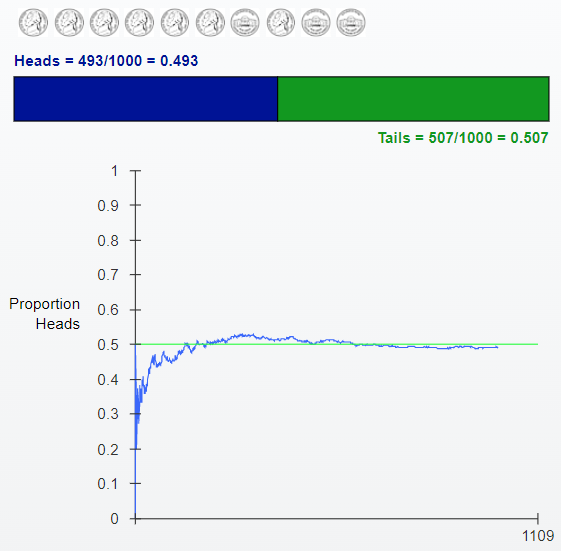
\includegraphics[width=0.8\textwidth]{Figures/Law-Large-Number.png}

Source:
\url{http://digitalfirst.bfwpub.com/stats_applet/stats_applet_10_prob.html}

\end{example}


\hypertarget{fundamental-properties-that-define-probability}{%
\subsection{Fundamental Properties (that Define
Probability)}\label{fundamental-properties-that-define-probability}}

\begin{itemize}
\item
  \textbf{Property 1:} For an event \(E\), the probability \(P(E)\) is
  ranged from 0 to 1: \[0\leq P(E)\leq 1.\]
\item
  \textbf{Property 2:} If \(S\) is the sample space, then \(P(S)=1\).
\item
  \textbf{Property 3:} The probability of an event
  \(E=\{e_1,e_2, \cdots e_k\}\) of distinct outcome is equal to the sum
  of probabilities of individual outcomes:
  \[P(E)=P(e_1)+P(e_2)+\cdots+P(e_k)\] where \(P(e_i)\) is the
  probability of getting the outcome \(e_i\).
\end{itemize}

\begin{remark}

When an event \(E\) consists of infinitely many outcomes, the right hand
side of the equality in Property 3 will be an infinite sum.

\end{remark}


\begin{itemize}
\item
  \textbf{Easy consequence 1:} If events \(A\) and \(B\) are mutually
  exclusive, then \[P(A\cup B)=P(A)+P(B).\]
\item
  \textbf{Easy consequence 2:} The probability \(P(E)\) of an event
  \(E\) and the probability \(P(E^c)\) of the complement event \(E^c\)
  satisfies the identity: \[P(E)+P(E^c)=1.\]

  Equivalently, \[
  P(E^c)=1-P(E)\quad\text{or}\quad P(E)=1-P(E^c).
  \]
\end{itemize}

\begin{example}

A six-sided fair die is rolled. Denote by \(E\) the event of getting a
number less than \(3\).

\begin{enumerate}
\item
  Find the probability \(P(E)\) of the event \(E\).
\item
  Find the probability \(P(E^c)\) of the complement \(E^c\) of the event
  \(E\).
\item
  Verify that \(P(E)+P(E^c)=1\).
\end{enumerate}

\end{example}

\begin{example}

Two six-sided fair dice were rolled. Find the probability of getting two
numbers whose sum is at least 4.

\end{example}
\vspace*{5\baselineskip}

\begin{exercise}

Two six-sided fair dice were rolled. Find the probability of getting two numbers whose sum is at most 10.

\end{exercise}
% \vspace*{5\baselineskip}

\begin{exercise}

A bag of M\&M's has 4 red, 6 green, 2 blue, and 3 yellow M\&M's. What is the probability of randomly picking:

\begin{enumerate}
  \item a yellow?
  \item a blue or green?
  \item an orange?
\end{enumerate}
  
\end{exercise}

\hypertarget{the-addition-rule}{%
\subsection{The Addition Rule}\label{the-addition-rule}}

When outcomes in the sample spaces are equally likely,

\begin{itemize}
\item
  the \textbf{probability of the intersection} of two events is \[
  P(A\cap B)=\dfrac{\text{numbers of elements in } A\cap B}{\text{number of elements in the sample space }S}.
  \]
\item
  the \textbf{probability of the union} of two events is \[
  P(A\cup B)=\dfrac{\text{numbers of elements in } A\cup B}{\text{number of elements in the sample space }S}.
  \]
\end{itemize}

In general, the probability of the union of two events from a chance
experiment is defined by the basic rules and the addition rule.


\textbf{Addition Rule:} the probability of the union of two events
\(A\) and \(B\) is \[
P(A\cup B)=P(A)+P(B)-P(A\cap B).
\]

\begin{example}
  A card was randomly drew from a deck of 52 cards.
  
\begin{fullwidth}
  \centering
  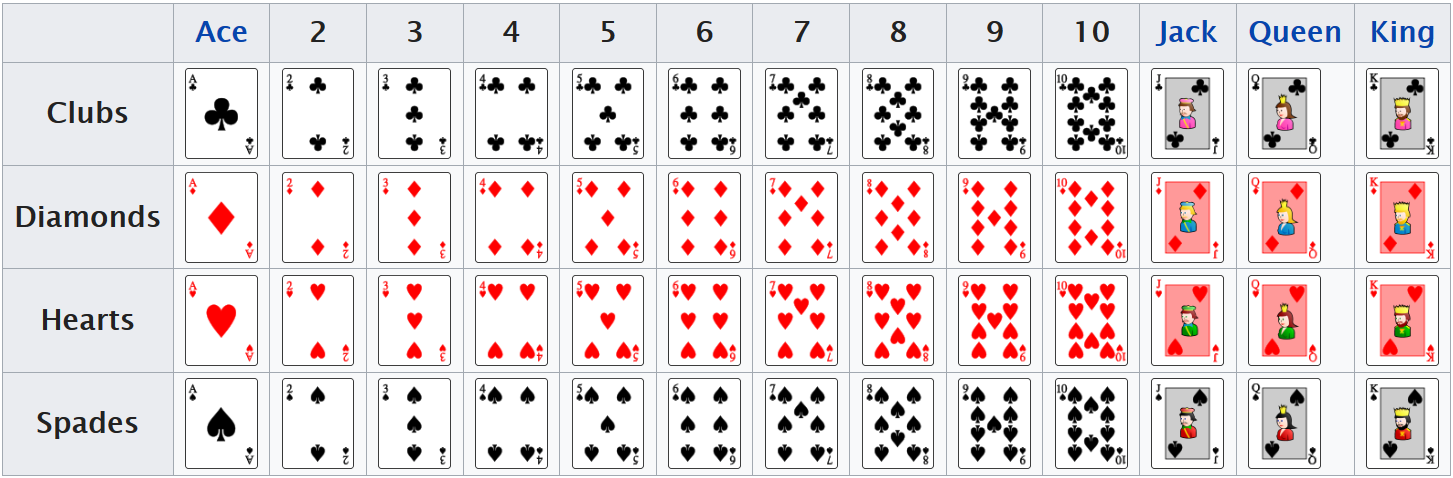
\includegraphics[width=\linewidth]{Figures/Standard-52-card-from-Wikipedia.png}
\end{fullwidth}  
  \begin{enumerate}
  \item
    What's the probability of getting a heart?
  \item
    What's the probability of getting a face?
  \item
    What's the probability of getting a heart face?
  \item
    What's the probability of getting a heart or a face?
  \item
    What's the probability of getting a club and spade?
  \end{enumerate}
\end{example}



\begin{exercise}

A jar contains 10 red marbles numbered 1 to 10 and 8 blue marbles numbered 1 to 8. A marble is drawn at random from the jar. Find the probability of the given event, please show your answers as reduced fractions.

\begin{enumerate}
  \item The marble is red.
  \item The marble is odd-numbered.
  \item The marble is blue or even-numbered.
  \item The marble is blue or even.
\end{enumerate}

\end{exercise}

\hypertarget{the-conditional-probability}{%
\subsection{The Conditional
Probability}\label{the-conditional-probability}}

\begin{itemize}
\item
  The \textbf{conditional probability} of \(A\) given \(B\), written as
  \(P(A\mid B)\), is the probability that event \(A\) will occur given
  that the event \(B\) has already occurred.
\item
  In the case that the chance experiment has equally likely outcomes,
  the conditional probability is, \[
  P(A\mid B)=\dfrac{\text{numbers of elements in }A\cap B}{\text{number of elements in }B}.
  \]
\item
  In general, we may use fundamental rules of probability and the
  multiplication rule to calculate the conditional probability.
\end{itemize}

\begin{example}

A fair die is rolled.

\begin{enumerate}
  \item 
  Find the probability that the number rolled is a five, given that it is odd.
  \item
  Find the probability that the number rolled is odd, given that it is a five.
\end{enumerate}

\end{example}

\hypertarget{the-multiplication-rule}{%
\subsection{The Multiplication Rule}\label{the-multiplication-rule}}

\begin{itemize}
\item
  \textbf{Multiplication Rule:} the probability of the intersection of
  two events \(A\) and \(B\) satisfies the following equality \[
  P(A\cap B)=P(B)P(A\mid B)=P(A)P(B\mid A).
  \]
\item
  The multiplication rule gives a formula for conditional probability:
  \[
  P(B\mid A)=\dfrac{P(A\cap B)}{P(A)}\qquad\qquad P(A\mid B)=\dfrac{P(A\cap B)}{P(B)}.
  \]
\end{itemize}


\begin{example}

  Consider flipping a fair coin and rolling a fair six-sided die together.
  
  \begin{enumerate}
  \item
    What's the probability that the coin shows a head?
  \item
    Given that a head occurs, what's the probability that the die shows a
    number bigger than 4?
  \item
    What's the probability of getting a head and a number bigger than 4?
  \item
    Verify that flipping a head and rolling a number bigger than 4 are
    independent events.
  \end{enumerate}
  
  \end{example}

\hypertarget{independent-events}{%
\subsection{Independent Events}\label{independent-events}}

\begin{itemize}
\item
  Two events \(A\) and \(B\) are \textbf{independent} if \[
  P(A\mid B)=P(A)\quad \text{ or }
  \quad P(B)=P(B\mid A).
  \] Equivalently, \[
  P(A\cap B)=P(A)P(B).
  \]
\item
  \textbf{Fundamental Counting Principle:} if there are \(m\) ways of
  doing something and \(n\) ways of doing another thing independently,
  then there are \(m\cdot n\) ways of performing both actions \emph{in
  order}.
\end{itemize}



\begin{example}

The probability that a student borrows a statistics book from the
library is 0.3. The probability that a student borrows a biology book is
0.4. Given that a student borrowed a biology book, the probability that
he/she borrows a statistics book is 0.6.

\begin{enumerate}
\item
  Find the probability that a student borrows a statistics book and a
  biology book.
\item
  Find the probability that a student barrows a statistics boor or a
  biology book.
\end{enumerate}

\end{example}

\hypertarget{sampling-with-replacement-or-without-replacement}{%
\subsection{Sampling with Replacement or without
Replacement}\label{sampling-with-replacement-or-without-replacement}}

\begin{itemize}
\item
  \textbf{With replacement:} If each member of a population is replaced
  after it is picked, then that member has the possibility of being
  chosen more than once. When sampling is done with replacement, then
  events are considered to be independent, meaning the result of the
  first pick will not change the probabilities for the second pick.
\item
  \textbf{Without replacement:} When sampling is done without
  replacement, each member of a population may be chosen only once. In
  this case, the probabilities for the second pick are affected by the
  result of the first pick. The events are considered to be dependent.
\end{itemize}

\begin{example}

Two cards were randomly drawn from a standard deck of 52 cards
\emph{with replacement}. Find the probability of getting exactly one
club card.

\end{example}
\vspace*{6\baselineskip}

\begin{example}

Two cards were randomly drawn from a standard deck of 52 cards without
replacement, which means the first card will not be put back.

\begin{enumerate}
\item
  Find the probability that getting two spades.
\item
  Find the probability that getting exactly one spade card.
\end{enumerate}

\end{example}

\begin{exercise}

A hacker is trying to guess someone's password. The hacker knows (somehow) that the password is 11 characters long, and that each character is either a lowercase letter, (a, b, c, etc), an uppercase letter (A, B, C, etc) or a numerical digit (0, 1, 2, 3, 4, 5, 6, 7, 8, or 9). Assume that the hacker makes random guesses.

What is the probability that the hacker guesses the password on his first try?

\end{exercise}
\vspace*{6\baselineskip}

\begin{exercise}

A special deck of 16 cards has 4 that are blue, 4 yellow, 4 green, and 4
red. The four cards of each color are numbered from one to four. A
single card is drawn at random. Find the following probabilities.

\begin{enumerate}
\item
  The probability that the card drawn is red.
\item
  The probability that the card is red, given that it is not green.
\item
  The probability that the card is red, given that it is neither red nor
  yellow.
\item
  The probability that the card is red, given that it is not a four.
\end{enumerate}

\end{exercise}

\begin{exercise}

  Use the following probabilities of event $A$ and $B$  
  $P(A)=0.33$, $P(B)=0.47$ and $P(A\text{~and~}B)=0.20$
  to find the probability $P(B\mid A^c)$.

\end{exercise}
\vspace*{6\baselineskip}

\begin{exercise}

A box contains 10 pens, 6 black and 4 red. Two pens are drawn without
replacement, which means that the first one is not put back.

\begin{enumerate}
\item
  What is the probability that both pens are red?
\item
  What is the probability that at most one pen is red?
\item
  What is the probability that at least one pen is red?
\end{enumerate}

\end{exercise}


\newlecture

% !TeX root = main.tex

\hypertarget{discrete-random-variables}{%
\section{Discrete Random Variables}\label{discrete-random-variables}}

\hypertarget{random-variables}{%
\subsection{Random Variables}\label{random-variables}}

\begin{itemize}
\item
  A \textbf{random variable}, usually written \(X\), is a variable whose
  values are numerical quantities of possible outcomes a random
  experiment.
\item
  A \textbf{discrete random variable} takes on only a finite or
  countable number of distinct values.
\item
  A \textbf{continuous random variable} takes on values which form an
  interval of numbers.
\end{itemize}

\begin{example}

\begin{itemize}
\item
  Rolling a fair dice, the number of dots on the top faces is a discrete
  random variables takes on the possible values: 1, 2, 3, ,4, 5, 6.
\item
  Flipping a fair coin 10 times, the number of heads is a discrete
  random variable takes on the possible values: 1, 2, 3, \ldots, 10.
\end{itemize}

\end{example}

\begin{example}

\begin{itemize}
\item
  The height of an randomly select 10 year-old boy in US is normally
  between 129 cm and 157 cm. So the height is a continuous random
  variable.
\item
  The measure the voltage at an randomly electrical outlet normally is
  between 118 and 122. So the measure of voltage is a continuous random
  variable.
\end{itemize}

\end{example}

\begin{exercise}

Classify each random variable as either discrete or continuous.

\begin{enumerate}
\item
  The number of boys in a randomly selected three-child family.
\item
  The temperature of a cup of coffee served at a restaurant.
\item
  The number of math majors in randomly selected group of 10 students.
\item
  The amount of rain recorded in a small town one day.
\end{enumerate}

\end{exercise}

\hypertarget{probability-distributions}{%
\subsection{Probability Distributions}\label{probability-distributions}}

\begin{itemize}
\item
  The \textbf{probability distribution} of a discrete random variable
  \(X\) is defined by the probability \(P(X=x)\) associated with each
  possible value \(x\) of the variable \(X\). The function
  \(p_X(x)=P(X=x)\) is called the \textbf{probability mass function}.
\item
  A probability distribution of a discrete random variable is usually
  characterized by a table of all possible values \(X\) together with
  probabilities \(P(X)\), or a probability histogram, or a formula.
\item
  A random variable \(X\) (discrete and continuous) always has a
  \textbf{cumulative distribution function}: \(F_X(x)=P(X\leq x)\) (=
  \(\sum\limits_{x_i\leq x} P(x_i)\) if \(X\) is discrete).
\end{itemize}

\hypertarget{basic-properties-of-probability-distributions}{%
\subsection{Basic Properties of Probability
Distributions}\label{basic-properties-of-probability-distributions}}

\begin{itemize}
\item
  Basic rules of probability:

  \begin{itemize}
  \item
    \(0\leq P(X=x)\leq 1\).
  \item
    the sum of all the probabilities is 1, that is
    \(P(X\leq x_{max})=1\).
  \item
    In particular, \(0\leq F_X(x)\leq 1\).
  \item
    The cumulative distribution function \(F_X(x)\) is non-decreasing.
  \end{itemize}
\item
  The probability distribution can be recovered from its cumulative
  distribution function. Indeed, for a \emph{discrete} random variable
  \(X\), we have \[P(X=x_i)=P(X\le x_i)-P(X\le x_{i-1}),\] where
  \(P(X\le x_i)=\sum\limits_{k=1}^i P(X=x_k)\).
\end{itemize}

\begin{example}

Let \(X\) be the number of heads that are observed when tossing two fair
coins.

\begin{enumerate}
\item
  Construct the probability distribution for \(X\).
\item
  Find \(P(X\le 1)\) and \(P(X\le 2)\).
\end{enumerate}

\end{example}

\begin{example}

The probability distribution of an unfair coin is characterized by the
following histogram. Find the probability of getting at most 1 head.

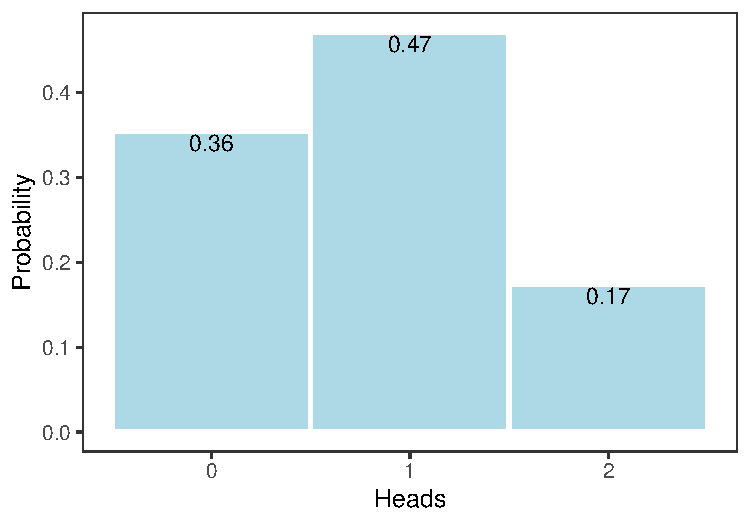
\includegraphics[width=\textwidth]{figure-latex/unnamed-chunk-7-2-1}

\end{example}

\begin{exercise}

A pair of fair 6-sided dice were rolled. Let \(X\) denote the sum of the
number of dots on the top faces.

\begin{enumerate}
\item
  Construct the probability distribution of \(X\).
\item
  Find the probability that \(X\) takes an odd value.
\end{enumerate}

\end{exercise}

\begin{exercise}

The number \(X\) of days in the summer months that a construction crew
cannot work because of the weather has the probability distribution

\begin{longtable}[]{@{}llllllllll@{}}
\toprule()
x & 6 & 7 & 8 & 9 & 10 & 11 & 12 & 13 & 14 \\
\midrule()
\endhead
P(x) & 0.03 & 0.08 & 0.15 & 0.2 & 0.19 & 0.16 & 0.1 & 0.07 & 0.02 \\
\bottomrule()
\end{longtable}

\begin{enumerate}
\item
  Find the probability that no more than ten days will be lost next
  summer.
\item
  Find the probability that from 8 to 12 days will be lost next summer.
\item
  Find the probability that no days at all will be lost next summer.
\end{enumerate}

\end{exercise}

\hypertarget{mean-and-standard-deviation-of-a-discrete-random-variable}{%
\subsection{Mean and Standard Deviation of a Discrete Random
Variable}\label{mean-and-standard-deviation-of-a-discrete-random-variable}}

Let \(X\) be a discrete random variable and \(p_X(x)=P(X=x)\) the
probability mass function.

\begin{itemize}
\item
  The \textbf{expected value} \(E(X)\) (also called \textbf{mean} and
  denoted by \(\mu\)) of the discrete random variable \(X\) is the
  number \[\mu=E(X)=\sum xp_X(x).\]
\item
  The \textbf{variance} \(\mathrm{Var}(X)\) (also denoted by
  \(\sigma^2\)) of the discrete random variable \(X\) is the number
  \[\sigma^2=\mathrm{Var(X)}=\sum (x-E(X))^2p_X(x).\]
\item
  The \textbf{standard deviation} \(\sigma\) of a discrete random
  variable \(X\) is the square root of its variance:
  \[\sigma=\sqrt{\sum (x-E(X))^2p_X(x)}.\]
\end{itemize}

\begin{example}

One thousand raffle tickets are sold for \$2 each. Each has an equal
chance of winning. First prize is \$500, second prize is \$300, and
third prize is \$100. Find the expected value of net gain, and interpret
its meaning.

\end{example}

\begin{example}

The wait times (rounded to multiples of 5) in the cafeteria at a
Community College has the following probability distribution. Find the
expected waiting time and the standard deviation.

\begin{longtable}[]{@{}llllll@{}}
\toprule()
\(x\) (minutes) & 5 & 10 & 15 & 20 & 25 \\
\midrule()
\endhead
\(P(X=x)\) & 0.13 & 0.25 & 0.31 & 0.21 & 0.1 \\
\bottomrule()
\end{longtable}

\end{example}

\begin{example}

The probability distribution of an unfair die is given in the following
table.

\begin{longtable}[]{@{}llllll@{}}
\toprule()
\(x\) & 1 & 2 & 3 & 4 & 5 \\
\midrule()
\endhead
\(P(X=x)\) & 0.18 & 0.12 & \(\,?\,\) & 0.14 & 0.23 \\
\bottomrule()
\end{longtable}

\begin{enumerate}
\item
  Find \(P(X=3)\).
\item
  Find the mean, variance and standard deviation of this probability
  distribution.
\end{enumerate}

\end{example}

\begin{exercise}

Seven thousand lottery tickets are sold for \$5 each. One ticket will
win \$2,000, two tickets will win \$750 each, and five tickets will win
\$100 each. Let \(X\) denote the net gain from the purchase of a
randomly selected ticket.

\begin{enumerate}
\item
  Construct the probability distribution of \(X\).
\item
  Compute the expected value \(E(X)\) of \(X\). Interpret its meaning.
\item
  Compute the standard deviation \(\sigma\) of \(X\).
\end{enumerate}

\end{exercise}

\hypertarget{binomial-distribution}{%
\subsection{Binomial Distribution}\label{binomial-distribution}}

\begin{itemize}
\item
  A \textbf{binomial experiment} is a probability experiment satisfying:

  \begin{enumerate}
  \item
    The experiment has a fixed number \(n\) of independent trials.
  \item
    Each trial has only two possible outcomes: a success (S) or a
    failure (F).
  \item
    The probability \(p\) of a success is the same for each trial.
  \end{enumerate}
\item
  The discrete random variable \(X\) counting the number of successes in
  the \(n\) trials is the \textbf{binomial random variable}. We say
  \(X\) has a \textbf{binomial distribution} with parameters \(n\) and
  \(p\) and write it as \(X\sim B(n, p)\).
\item
  For \(X\sim B(n, p)\), the \textbf{probability of getting exactly
  \(x\) successes in \(n\) trials} is
  \[P(X=x)=B(x,n,p)={_n C_x} p^x(1-p)^{n-x}=\frac{n!}{(n-x)!x!}p^x(1-p)^{n-x},\]
  where \(n!=n(n-1)\cdots 1\), read as \(n\) factorial, for \(n>0\) and
  \(0!=1.\)
\item
  The notation \({_n C_x}=\frac{n!}{(n-x)!x!}\) is read as \(n\) choose
  \(x\), which is the number of ways to choose \(x\) objects from a set
  of \(n\) objects.
\end{itemize}

\begin{example}

A card is randomly selected from a standard deck and replaced. This
experiment is repeated a total of \(5\) times.

\begin{itemize}
\item
  Find the probability of getting exactly \(3\) clubs.
\item
  Find the probability of getting at least \(3\) clubs.
\end{itemize}

\end{example}

\begin{exercise}

Let \(X\) be a binomial random variable with parameters \(n = 5\),
\(p=0.2\). Find the probabilities

\begin{enumerate}
\item
  \(P(X=3),\)
\item
  \(P(X<3),\)
\item
  \(P(X>3).\)
\end{enumerate}

\end{exercise}

\begin{exercise}

A manufacturing machine has a 4\% defect rate.

If 6 items are chosen at random, what is the probability that at least
one will have a defect?

\end{exercise}

\hypertarget{mean-and-standard-deviation-of-binomial-distribution}{%
\subsection{Mean and Standard Deviation of Binomial
Distribution}\label{mean-and-standard-deviation-of-binomial-distribution}}

\begin{itemize}
\item
  The mean of a binomial distribution of \(n\) trials is
  \[\mu =\sum xP(X=x)=\sum x\cdot \dfrac{n!}{(n-x)!x!}p^x(1-p)^{n-x} = np.\]
\item
  The variance of a binomial distribution of \(n\) trials is
  \[\sigma^2 =\sum (x-np)^2P(X=x)=\sum x^2P(X=x)-(np)^2=np(1-p).\]
\item
  The standard deviation of a binomial distribution of \(n\) trials is
  \[\sigma=\sqrt{np(1-p)}.\]
\item
  We consider an event \(E\) \textbf{unusual} if the probability
  \(P(E)\leq 5\%\).
\end{itemize}

\begin{example}

The probability that an egg in a retail package is cracked or broken is
0.02.

\begin{enumerate}
\item
  Find the average number of cracked or broken eggs in a one dozen
  carton.
\item
  Find the standard deviation.
\item
  Is getting at least two broken eggs unusual?
\end{enumerate}

\end{example}

\begin{exercise}

Adverse growing conditions have caused 5\% of grapefruit grown in a
certain region to be of inferior quality. Grapefruit are sold by the
dozen.

\begin{enumerate}
\item
  Find the average number of inferior quality grapefruit per box of a
  dozen.
\item
  A box that contains two or more grapefruit of inferior quality will
  cause a strong adverse customer reaction. Find the probability that a
  box of one dozen grapefruit will contain two or more grapefruit of
  inferior quality.
\end{enumerate}

\end{exercise}

\begin{exercise}

CCA has stated in 2017 that 48\% of its students are first generation
college students.

Suppose you sample 5 CCA students and ask if they are first generation
college students or not, counting the number of first generation
students.

\begin{enumerate}
\item
  Create a binomial probability distribution (table) for this situation.
\item
  Find the mean of the binomial distribution.
\item
  Find the standard deviation of this binomial distribution.
\end{enumerate}

\end{exercise}

\hypertarget{extra-practice-problems}{%
\subsection{Extra Practice Problems}\label{extra-practice-problems}}

\begin{exercise}

Find the mean and the standard deviation of the probability
distribution.

\begin{tabular}{ll}
\toprule
x & P(x) \\
\midrule
0 & 0.2 \\
1 & 0.2 \\
2 & 0.1 \\
3 & 0.5 \\
\bottomrule
\end{tabular}

\end{exercise}

\begin{exercise}

A company tracks the number of sales new employees make each day during
a 100-day probationary period. The results for one new employee are
shown at the right.

\begin{tabular}{@{}ll@{}}
  \toprule
  Sales per day \(x\) & Number of days \(f\) \\
  \midrule
  0 & 16 \\
  1 & 19 \\
  2 & 15 \\
  3 & 21 \\
  4 & 9 \\
  5 & 10 \\
  6 & 8 \\
  7 & 2 \\
  \bottomrule
  \end{tabular}

\begin{enumerate}
\item
  Find the probability of each outcome.
\item
  Construct a probability distribution table.
\item
  Find the mean of the probability distribution.
\item
  Find the variance and standard deviation.
\end{enumerate}

\end{exercise}

\begin{exercise}

A poll is given, showing 35\% are in favor of a new building project.

If 5 people are chosen at random, what is the probability that exactly 2
of them favor the new building project?

\end{exercise}
\vspace*{5\baselineskip}

\hypertarget{lab-binomial-distribution}{%
\subsection{Lab: Binomial
Distribution}\label{lab-binomial-distribution}}

Let \(X\) be a binomial random variable with parameters \(n\) and \(p\), that is \(X\sim B(n, p)\). In Excel, \(P(X=x)\) is given by\\
\texttt{BINOM.DIST(x,\ n,\ p,\ FALSE)}\\
 and \(P(X\le x)\) is given by\\
\texttt{BINOM.DIST(x,\ n,\ p,\ TRUE)}.\\
You may click input function
\(f_x\) and then search \texttt{binom} to find the function.

\begin{exercise}

A type of surgery has a 90\% chance of success. The surgery is performed
on 7 patients.

Use excel to answer the following questions.

\begin{enumerate}
\item
  Find the probability of the surgery being successful on exactly 5
  patients.
\item
  Find the probability of the surgery being successful on at least 4
  patients.
\end{enumerate}

\end{exercise}


\newlecture

% !TeX root =  main.tex

\section{Discrete Random Variables}

\hypertarget{probability-distribution-of-a-continuous-random-variable}{%
\subsection{Probability Distribution of a Continuous Random
Variable}\label{probability-distribution-of-a-continuous-random-variable}}

\begin{itemize}
\item
  The probability distribution of a continuous random variable \(X\) is
  characterized by its \textbf{probability density function} \(f(X)\)
  satisfying that the probability \(P(a\leq X\leq b)\) equals the area
  above the interval \([a, b]\) but under the graph of the density
  function \(f(X)\) which is also called a \textbf{density curve}.
\end{itemize}

\begin{fullwidth}
  \colorbox{white}{
    \parbox{\linewidth}{
      \begin{multicols*}{2}
        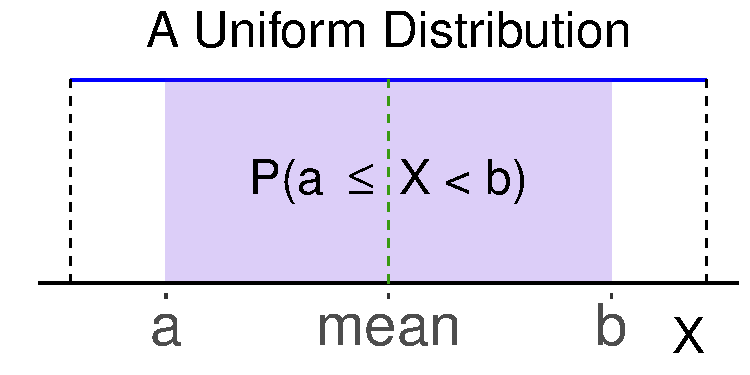
\includegraphics[width=0.8\linewidth]{figure-latex/unnamed-chunk-8-2-1}
        
        \columnbreak

        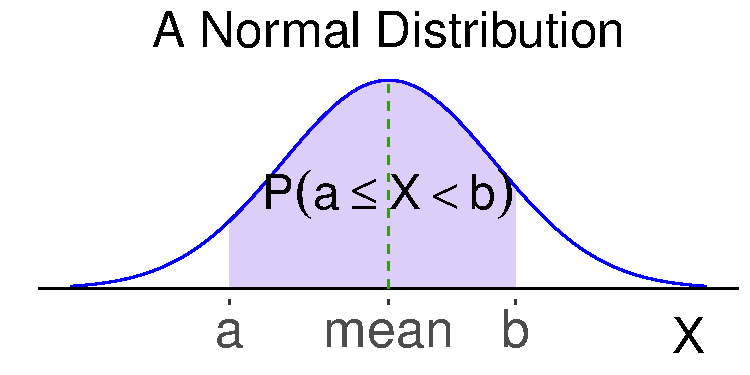
\includegraphics[width=0.8\linewidth]{figure-latex/unnamed-chunk-8-3-1}
      \end{multicols*}
    }}
\end{fullwidth}

\hypertarget{properties-of-probability-distribution-of-a-continuous-random-variable}{%
\subsection{Properties of Probability Distribution of a Continuous
Random
Variable}\label{properties-of-probability-distribution-of-a-continuous-random-variable}}

\begin{itemize}
\item
  The probability density function \(f\) is nonnegative, that is
  \(f(X)\ge 0\).
\item
  The total area under a density curve is 1.
\item
  The cumulative probability \(P(X\le b)\) of a random variable \(X\)
  equals the area under the density curve to the left side of \(b\).
\item
  By the addition rule of probability, we have
    \[P(a\le X\le b)=P(X\le b)-P(X\le a)\]
    \[P(X\ge b)=1-P(X\le b)\]
\item
  As a line segment has no area, we have \(P(X\le a)=P(X< a)\) as well
  as \(P(X\ge b)=P(X>b)\)
\end{itemize}

\begin{example}

Let \(X\) be the amount of time that a commuter must wait for a train.
Suppose \(X\) has a probability density function \[
f(X)=
\begin{cases}
  0.1, & 0\leq X\leq 10\\
  0,   & \text{otherwise}
\end{cases}
\]

What is the probability that the commuter's waiting time is less than 4
minutes?

\end{example}

\vspace*{4\baselineskip}

\hypertarget{normal-distribution}{%
\subsection{Normal Distribution}\label{normal-distribution}}

\begin{itemize}
\item
  A \textbf{normal distribution} has a \textbf{density function}
  \[f(x)=\frac{1}{\sqrt{2\pi \sigma^2}}e^{-\frac{(x-\mu)^2}{2\sigma^2}},\]
  where \(\mu\) is the mean, \(\sigma\) is the standard deviation,
  \(\pi\approx 3.14159\) and \(e\approx 2.71828\). The graph of \(f\) is
  called a \textbf{normal curve}.
\item
  We write \(X\sim N(\mu, \sigma^2)\) for a normal random variable \(X\)
  with the mean \(\mu\) and the standard deviation \(\sigma\).
\item
  A normal distribution has the following properties:

  \begin{itemize}
  \item
    \emph{The mean, median, and mode are equal}.
  \item
    The normal curve is \emph{bell shaped and \textbf{symmetric}} with
    respect to the mean.
  \item
    The \emph{total area} under the curve and above the \(x\)-axis is
    \(1\).
  \item
    The normal curve \emph{approaches, but never touches, the
    \(x\)-axis} as \(x\) goes to \(\pm\infty\).
  \item
    Between \(\mu-\sigma\) and \(\mu+\sigma\), the graph \emph{curves
    downward}. On the left side of \(\mu-\sigma\) or the right side of
    \(\mu+\sigma\), the graph \emph{curves upward}. A point at which the
    curve changes the direction of curving is called an
    \textbf{inflection point}.
  \end{itemize}
\end{itemize}

\begin{fullwidth}
  \colorbox{white}{
    \parbox{\linewidth}{
  \centering
  \textbf{Normal Curves with Different Means and Standard Deviations}

  \begin{multicols*}{2}
    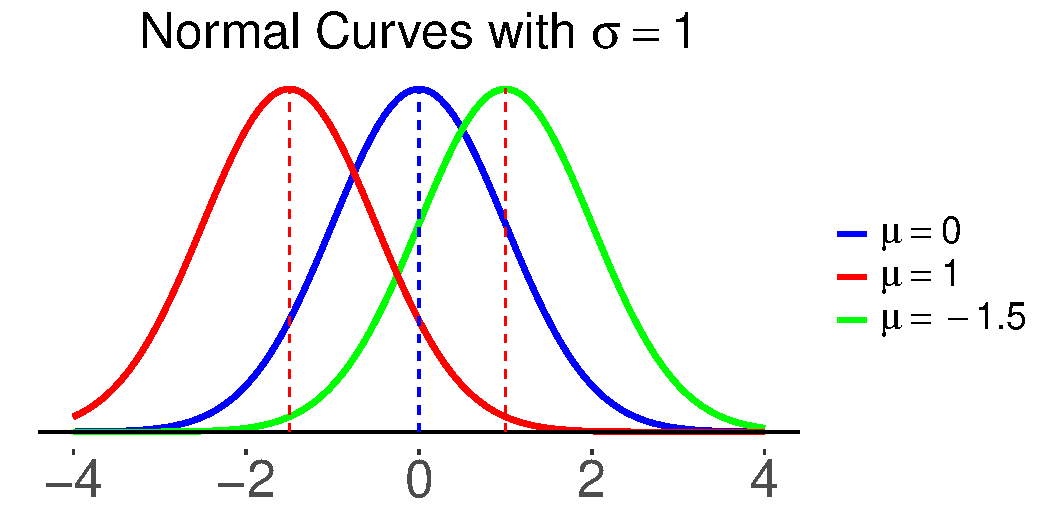
\includegraphics[width=0.8\linewidth]{figure-latex/unnamed-chunk-8-4-1}
    
    \columnbreak

    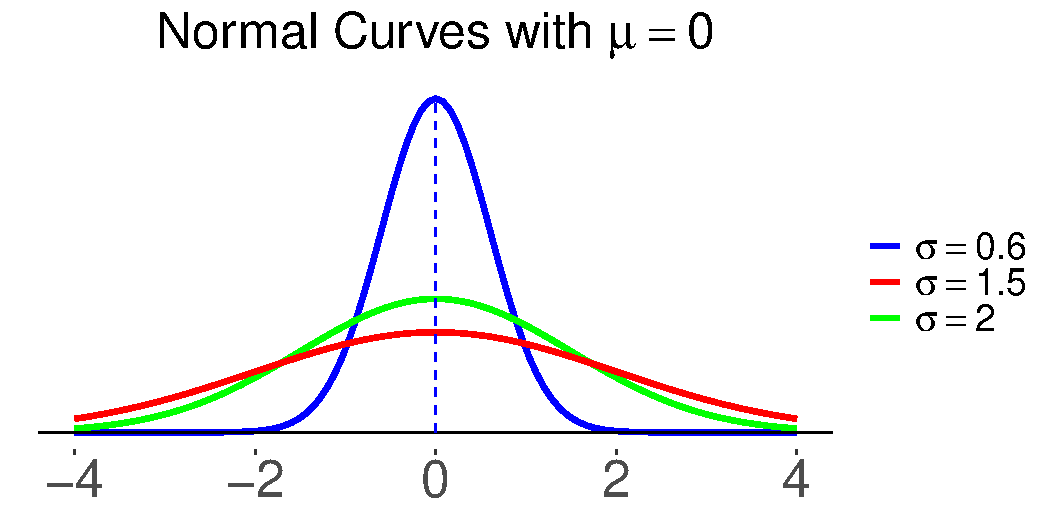
\includegraphics[width=0.8\linewidth]{figure-latex/unnamed-chunk-8-5-1}
  \end{multicols*}
    }}
\end{fullwidth}


\hypertarget{the-empirical-rule-for-normal-distributions}{%
\subsection{The Empirical Rule for Normal
Distributions}\label{the-empirical-rule-for-normal-distributions}}

For any normal distribution, the proportion of data values within 1, 2,
and 3 standard deviations away from the mean are approximately 68.3\%,
95.4\% and 99.7\% respectively.

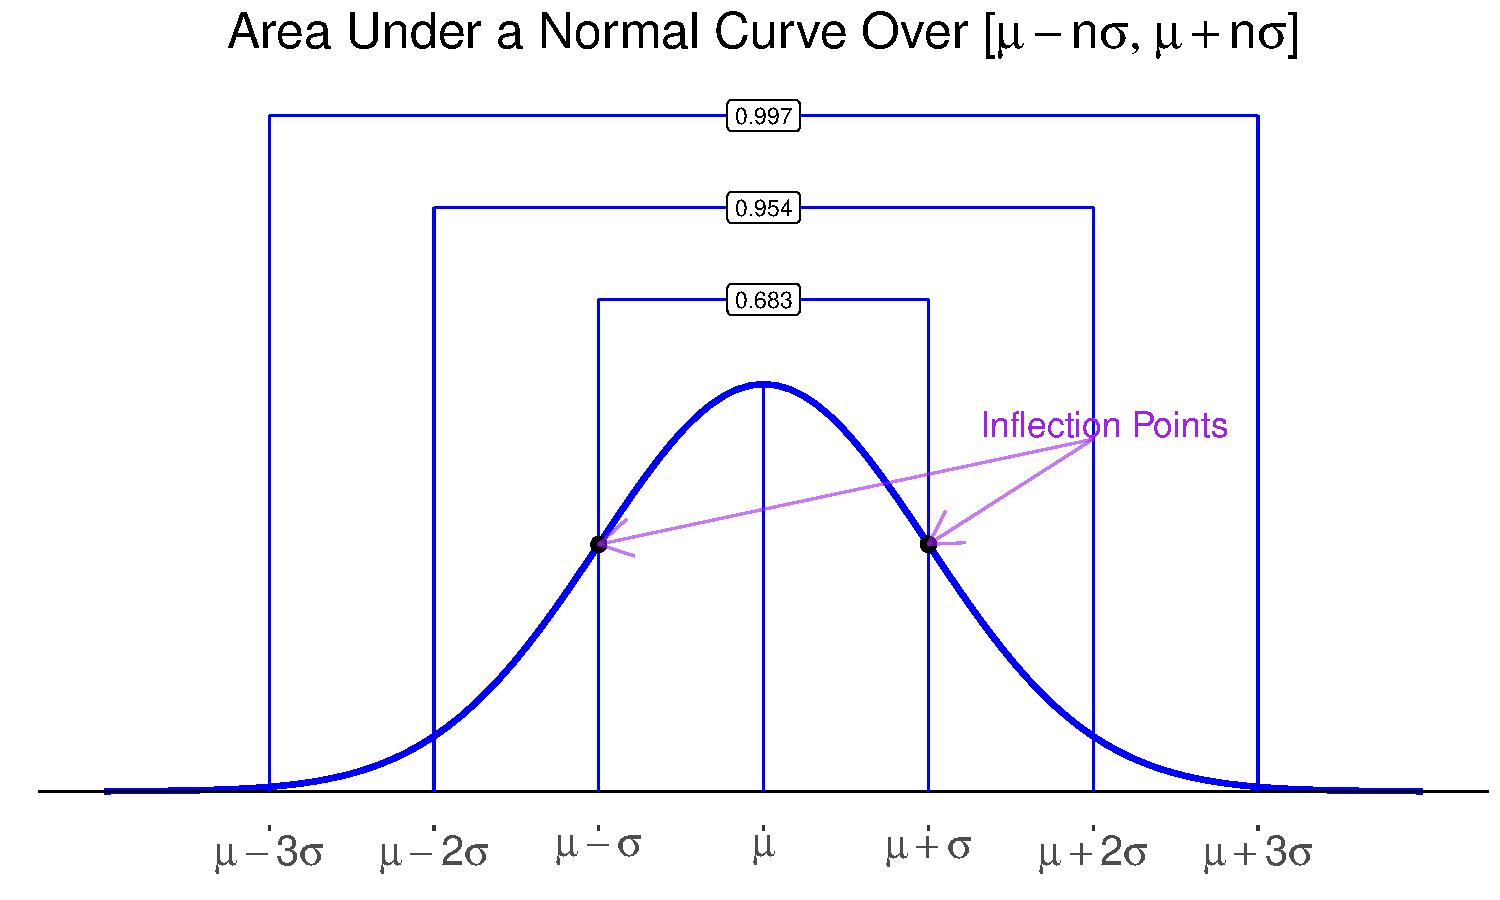
\includegraphics[width=0.8\textwidth]{figure-latex/unnamed-chunk-8-6-1}

\begin{example}

Suppose that foot length of a randomly chosen adult male is a normal
random variable with the mean \(\mu=11\) and the standard deviation
\(\sigma=1.5\).

\begin{enumerate}
\item
  How likely is a male's foot length to be smaller than 9.5 inches
\item
  How likely is a male's foot length to be bigger than 8 inches
\end{enumerate}

\end{example}

\hypertarget{standard-normal-distribution}{%
\subsection{Standard Normal
Distribution}\label{standard-normal-distribution}}

\begin{itemize}
\item
  A normal distribution is called a \textbf{standard normal
  distribution} if the mean is \(\mu=0\) and the standard deviation is
  \(\sigma=1\).
\item
  A random normal variable can be \textbf{standardized} by the following
  formula \(z=\frac{x-\mu}{\sigma}.\) We call the value \(z\) the
  \(Z\)-\textbf{score} of \(x\). In Excel, the \(Z\)-score of \(x\) can
  be calculated using the function \texttt{STANDARDIZE()}.
\item
  Standardization preserves probability:
  \[P(a<X<b)=P\left(\frac{a-\mu}{\sigma}< Z < \frac{b-\mu}{\sigma}\right).\]
\item
  The probability \(P(Z< z)\) of a standard normal random variable \(Z\)
  can be found using the Excel function \texttt{NORM.S,DIST(z,\ TRUE)}.
\item
  The probability \(P(X< x)\) of a normal random variable \(X\) can be
  calculated using the Excel function
  \texttt{NORM.DIST(x,\ mean,\ sd,\ TRUE)}.
\end{itemize}

\begin{example}

Let \(X\) be a norma random variable with the mean \(\mu = 8\) and the
standard deviation \(\sigma=2\).

\begin{enumerate}
\item
  Find the \(Z\)-score for the value \(X=13\).
\item
  Find the \(X\)-value for the \(Z\)-score \(z=-0.6\).
\end{enumerate}

\end{example}

\begin{example}

Let \(Z\) be a standard normal random variable.

\begin{enumerate}
\item
  Find \(P(Z<1.21)\).
\item
  Find \(P(Z\geq 1.21)\).
\item
  Find \(P(0<Z\leq 1.21)\).
\end{enumerate}

\end{example}

\begin{example}

The heights of 25-year-old women in a certain region are approximately
normally distributed with mean 62 inches and standard deviation 4
inches. Find the probability that a randomly selected 25-year-old woman
is more than 67 inches tall.

\end{example}
\vspace*{5\baselineskip}

\hypertarget{cutoff-value-for-a-given-tail-area}{%
\subsection{Cutoff Value for a Given Tail
Area}\label{cutoff-value-for-a-given-tail-area}}

\begin{itemize}
\item
  The \(k\)-th percentile for a random variable \(X\) is the value
  \(x_k\) that cuts off a left tail with the area \(k/100\), that is
  \(P(X<x_k)=\frac{k}{100}\), where \(0\leq k\leq 100\).
\item
  Let \(c\) be a nonnegative number less than or equal to 1. The
  \((100c)\)-th percentile for the standard normal distribution is
  usually denoted as \(-z_c\), that is \(P(Z<-z_c)=c\). By symmetry,
  \(z_c\) is the value such that \(P(Z> z_c)=c\), that is
  \(P(Z<z_c)=1-c\).
\item
  For a normal random variable \(X\) with the mean \(\mu\) and standard
  deviation \(\sigma\), the cutoff value \(x^*\) with a \textbf{tail
  area} \(c\), can be calculated using the standardization formula, that
  is, \[x^*=z^*\cdot \sigma+\mu,\] where \(z^*\) is the cutoff
  \(z\)-score with the tail area \(c\), that is \(z^*=-z_c\) given that
  \(c\) is the left-tail area and \(z^*=z_c\) given that \(c\) is the
  right tail area.
\end{itemize}

\begin{example}

Let \(X\) be the normal random variable with mean \(6\) and standard
deviation \(3\). Suppose the value \(x^*\) cuts off a left-tail area
\(0.05\). Find the value \(x^*\).

\end{example}
\vspace*{4\baselineskip}

\begin{example}

Scores on a standardized college placement examination are normally
distributed with mean 60 and standard deviation 13. Students whose
scores are in the top 5\% will be placed in a Calculus II course. Find
the minimum score needed to be placed in a Calculus II course.

\end{example}
\vspace*{6\baselineskip}

\begin{exercise}

A man arrives at a bus stop at a random time (that is, with no regard for the scheduled service) to catch the next bus. Buses run every  30  minutes without fail, hence the next bus will come any time during the next  30  minutes with evenly distributed probability (a uniform distribution). Find the probability that a bus will come within the next  10  minutes.

\end{exercise}
\vspace*{6\baselineskip}

\begin{exercise}

\begin{enumerate}
\item
  Let \(Z\) be a standard normal random variable. Find the
  probabilities:
  \[\text{1.}\,\, P(Z<1.58)\quad \text{2.}\,\,  P(-0.6<Z<1.67)\quad \text{3.}\,\, P(Z>0.19).\]
\item
  Let \(X\) be a normal random variable with \(\mu=5\) and \(\sigma=2\).
  Find the probabilities:
  \[\text{1.}\,\,  P(-2<X<8)\quad \text{2.}\,\, P(X>-1) \quad \text{3.}\,\, P(X<4).\]
\end{enumerate}

\end{exercise}

\begin{exercise}

The lifetimes of the tread of a certain automobile tire are normally distributed with mean  37,500  miles and standard deviation  4,500  miles. Find the probability that the tread life of a randomly selected tire will be between  30,000  and  40,000  miles.

\end{exercise}
\vspace*{6\baselineskip}

\begin{exercise}

A manufacturer knows that their items have a normally distributed lifespan, with a mean of 9.6 years, and standard deviation of 3 years.

The 4\% of items with the shortest lifespan will last less than how many years?

\end{exercise}
\vspace*{6\baselineskip}

\begin{exercise}

The life of a particular battery is known to follow a normal distribution , with a mean of 1133 hours and a standard deviation of 105 hours.

\begin{enumerate}
  \item 
  What percent of batteries last less than 1033 hours?
  \item 
  The 86 th percentile is represented by what number of hours of battery life? 
  \item
  What is the probability that a randomly selected battery will last more than 1362 hours?
\end{enumerate}

\end{exercise}

\begin{exercise}

Let \(Z\) be a normal random variable with \(\mu=0\) and \(\sigma=1\).
Let \(X\) be a normal random variable with \(\mu=4.3\) and
\(\sigma=1.7\).

Determine the values \(P(Z>1) + P(X<6)\) and explain how do you find the
value.

\end{exercise}
\vspace*{4\baselineskip}

\hypertarget{lab-normal-distributions}{%
\subsection{Lab: Normal Distributions}\label{lab-normal-distributions}}

\begin{itemize}
\item
  Let \(Z\) be a standard normal random variable. In Excel, \(P(Z<z)\)
  is given by \texttt{NORM.S.DIST(z,\ TRUE)}.
\item
  Let \(X\) be a normal random variable with mean \(\mu\) and standard
  deviation \(\sigma\), that is \(X\sim N(\mu, \sigma^2)\). In Excel,
  \(P(X<x)\) is given by \texttt{NORM.DIST(x,\ mean,\ sd,\ TRUE)}.
\item
  When a cumulative probability \(p=P(X<x)\) of a normal random variable
  \(X\) is given, we can find \(x\) using
  \texttt{NORM.INV(p,\ mean,\ sd)}.
\item
  When a cumulative probability \(p=P(Z<z)\) of a standard normal random
  variable \(Z\) is given, we can find \(z\) using
  \texttt{NORM.S.INV(p)}.
\end{itemize}

\begin{exercise}
  Let $Z$ be a standard normal random variable. Find each of the following probabilities. \textbf{Write down the Excel function you used to do the calculation.}

  \begin{enumerate}[itemsep=2.5\baselineskip, after=\vspace*{2\baselineskip}]
    \item $P(Z<0.96)$
    \item $P(Z>-1.43)$
    \item $P(-0.47< Z \le 2.31)$
    \item $P(Z<1.23 \text{~or~} Z>2.13)$
  \end{enumerate}
\end{exercise}

\begin{exercise}
  Let $X$ be a normal random variable with mean  52  and standard deviation  7.
  Find each of the following probabilities. \textbf{Write down the Excel function you used to do the calculation.}

  \begin{enumerate}[itemsep=2.5\baselineskip, after=\vspace*{2\baselineskip}]
    \item $P(X<62)$
    \item $P(X> 35)$
    \item $P(41 < X < 58)$
    \item $P(X<51 \text{~or~} Z>67)$
  \end{enumerate}
\end{exercise}


\newlecture

% !TeX root = main.tex

\hypertarget{sampling-distributions}{%
\section{Sampling Distributions}\label{sampling-distributions}}

\begin{itemize}
\item
  When using sample statistics to estimate population parameter, there
  will be a chance error
  \[\text{Population Parameter}=\text{Sample Statistic}+\text{Chance Error}.\]
\item
  To understand the chance error, we need to know how sample statistics
  distribute. Consider samples of the same size \(n\) randomly chosen
  from the population with replacement.
\item
  The probability distribution of a sample statistic is called a
  \textbf{sampling distribution}.
\item
  The sampling distribution varies as the sample size changes. In
  general, A larger sample size will result a smaller standard deviation
  of the sampling distribution.
\item
  The standard deviation of a sampling distribution is also called the
  \textbf{standard error}.
\end{itemize}

\hypertarget{central-limit-theorem-for-mean}{%
\subsection{Central Limit Theorem for
Mean}\label{central-limit-theorem-for-mean}}

\begin{theorem}[The Central Limit Theorem]
As the sample size \(n\) increases, the sampling distribution of the
sample mean, from a population with the mean \(\mu\) and the standard
deviation \(\sigma\), will approach to a normal distribution with the
mean \(\mu_{\bar{X}}=\mu\) and the standard deviation
\(\sigma_{\bar{X}}=\dfrac{\sigma}{\sqrt{n}}\).
\end{theorem}

\begin{remark}
  \begin{itemize}
    \item 
  In terms of standardization, the central limit
    theorem says that the random variable
    \(\bar{Z}=\dfrac{\bar{x}-\mu}{\sigma/\sqrt{n}}\) has an approximately
    standard normal distribution.
  \item
    For most distributions (\textbf{not highly skewed}), when sample size \(n>30\),
    the sampling distribution of the sample mean \(\bar{X}\) can be
    approximated reasonably well by a normal distribution. The larger the
    sample size, the better the approximation will be.
  \item
    When the population is normally distributed, the sampling distribution of the sample means will be normally distributed for any sample size.
  \item
    If the population distribution is highly skewed, relying on CLT can be
    risky.
  \end{itemize}
\end{remark} 

See the discussion on intuitive explanation:
\url{https://bit.ly/3dtf0q0}

\begin{example}

Randomly draw samples of size 2 with replacement from the numbers 1, 3,
4.

\begin{enumerate}
\item
  Find the sampling distribution of sample means.
\item
  Find the mean, and standard deviation of the sample means.
\item
  Find the mean, and standard deviation of the population.
\item
  How are the means of the population and the sampling distribution
  related.
\item
  How are the standard deviations of the population and the sampling
  distribution related.
\end{enumerate}

\end{example}

\begin{example}

Suppose the mean length of time that a caller is placed on hold when
telephoning a customer service center is 23.8 seconds, with standard
deviation 4.6 seconds. Find the probability that the mean length of time
on hold in a random sample of 1,000 calls will be within 0.5 second of
the population mean.

\end{example}

\vspace*{6\baselineskip}

\begin{example}

Suppose speeds of vehicles on a particular stretch of roadway are
normally distributed with mean 36.6 mph and standard deviation 1.7 mph.

\begin{enumerate}
\item
  Find the probability that the speed \(X\) of a randomly selected
  vehicle is between 35 and 40 mph.
\item
  Find the probability that the mean speed \(\bar{X}\) of 10 randomly
  selected vehicles is between 35 and 40 mph.
\end{enumerate}

\end{example}

\hypertarget{sampling-distribution-of-a-sample-proportion}{%
\subsection{Sampling Distribution of a Sample
Proportion}\label{sampling-distribution-of-a-sample-proportion}}

The proportion of a specific characteristic in a data set can be viewed
as the mean of the data set by identifying the specific characteristic
with 1 and others with \(0\).

\begin{example}

Consider the following data set

\textbf{1}, 0, \textbf{1}, \textbf{1}, 0, 0, \textbf{1}, 0, \textbf{1},
\textbf{1}

\begin{enumerate}
\item
  What proportion of the numbers are in bold?
\item
  What's the mean of the data set?
\item
  Is there any relation between the proportion and the mean? If so,
  describe it.
\end{enumerate}

\end{example}

\begin{itemize}
  \item 
  In general, if a population consisting of 1s and 0s, then the proportion
  \(p\) of 1s is the same as the mean. The standard deviation is
  \[\sigma=\sqrt{(1-p)^2p+(0-p)^2(1-p)}=\sqrt{p(1-p)}.\]
\end{itemize}

\hypertarget{central-limit-theorem-for-proportion}{%
\subsection{Central Limit Theorem for
Proportion}\label{central-limit-theorem-for-proportion}}

For a sampling distribution of sample proportion, we write \(\hat{P}\)
for the random variable of sample proportions.

\begin{theorem}

\textbf{Central Limit Theorem for Proportion:}

For large samples, the distribution of sample proportions \(\hat{P}\) is
approximately normal, with the mean \(\mu_{\hat{P}}=p\) and the standard
deviation \(\sigma_{\hat{P}}=\sqrt{\frac{p(1-p)}{n}}\), where \(p\) is
the population proportion and \(n\) is the sample size.

\end{theorem}

\begin{itemize}
\item
  Because a sample proportion is always between 0 and 1, and 99.7\% of sample
  proportions lie within 3 standard deviation away from the population
  proportion. When using the central limit theorem for proportion, we
  require the sample size \(n\) satisfying the following condition: the
  interval
  \[\left[p-3\sqrt{\frac{p(1-p)}{n}}, p+3\sqrt{\frac{p(1-p)}{n}}\right]\]
  lies wholly in the interval \([0, 1]\).
\item
  In practice, if \(n\) satisfies the following two inequalities:
  \(np\ge 10\) and \(n(1-p)\ge 10\), then we consider \(n\) is large
  enough for assuming that the sampling distribution of the sample
  proportion is approximately normal.
\item
  When the population proportion \(p\) is unknown, to apply the central
  limit theorem for proportion, we require the sample size \(n\)
  satisfying the same conditions with \(p\) replaced by the sample
  proportion \(\hat{p}\). That is, the sample size \(n\) should
  satisfies \(n\hat{p}\ge 10\) and \(n(1-\hat{p})\ge 10\).
\end{itemize}

\begin{example}

Suppose that in a population of voters in a certain region 53\% are in
favor of a particular law. Nine hundred randomly selected voters are
asked if they favor the law.

Find the probability that the sample proportion computed from a random
sample of size 900 will be at least 2\% above true population
proportion.

\end{example}

\vspace*{6\baselineskip}

\begin{example}

Suppose that in 36\% of all car accidents involve injury. Find the
probability that the injury rate in a random sample of 250 car accidents
is between 30\% and 45\%.

\end{example}

\vspace*{6\baselineskip}

\begin{exercise}

An unknown distribution has a mean of 28 and a standard deviation 6.
Samples of size \(n = 40\) are drawn randomly from the population. Find the
probability that the sample mean is between 27 and 30.

\end{exercise}

\vspace*{6\baselineskip}

\begin{exercise}

The numerical population of grade point averages at a college has mean
2.61 and standard deviation 0.5. If a random sample of size 100 is taken
from the population, what is the probability that the sample mean will
be between 2.51 and 2.71?

\end{exercise}

\vspace*{6\baselineskip}

\begin{exercise}

An airline claims that 72\% of all its flights to a certain region
arrive on time. In a random sample of 30 recent arrivals, 19 were on
time. You may assume that the normal distribution applies.

\begin{enumerate}
\item
  Compute the sample proportion.
\item
  Assuming the airline's claim is true, find the probability of a sample
  of size 30 producing a sample proportion so low as was observed in
  this sample.
\end{enumerate}

\end{exercise}

\begin{exercise}

In a mayoral election, based on a poll, a newspaper reported that the
current mayor received 45\% of the vote. If this is true, what is the
probability that a random sample of 100 voters had less than 35\% voting
for the current mayor?

\end{exercise}

\vspace*{6\baselineskip}

\hypertarget{more-practice-on-sampling-distributions}{%
\subsection{More Practice on Sampling
Distributions}\label{more-practice-on-sampling-distributions}}

\begin{exercise}

A population has the mean 73.5 and the standard deviation 2.5.

\begin{enumerate}
\item
  Find the mean and standard deviation of \(\bar{X}\) for samples of
  size 40.
\item
  Find the probability that the mean of a sample of size 40 will be less
  than 72.
\end{enumerate}

\end{exercise}

\begin{exercise}

A normally distributed population has the mean 57.7 and the standard deviation
12.1.

\begin{enumerate}
\item
  Find the probability that a single randomly selected element X of the
  population is less than 45.
\item
  Find the mean and standard deviation of \(\bar{X}\) for samples of
  size 16.
\item
  Find the probability that the mean of a sample of size 16 drawn from
  this population is less than 45.
\end{enumerate}

\end{exercise}

\begin{exercise}

Suppose the mean amount of cholesterol in eggs labeled ``large'' is 186
milligrams, with the standard deviation 7 milligrams. Find the probability
that the mean amount of cholesterol in a sample of 144 eggs will be
within 2 milligrams of the population mean.

\end{exercise}

\vspace*{6\baselineskip}

\begin{exercise}

Suppose that 8\% of all males suffer some form of color blindness. Find
the probability that in a random sample of 250 men at least 10\% will
suffer some form of color blindness.
  
\end{exercise}

\vspace*{6\baselineskip}

\begin{exercise}

An airline claims that 72\% of all its flights to a certain region
arrive on time. In a random sample of 30 recent arrivals, 19 were on
time. You may assume that the normal distribution applies.

\begin{enumerate}
\item
  Compute the sample proportion.
\item
  Assuming the airline's claim is true, find the probability of a sample
  of size 30 producing a sample proportion so low as was observed in
  this sample.
\end{enumerate}

\end{exercise}

\begin{exercise}

A particular fruit's weights are normally distributed, with a mean of
663 grams and a standard deviation of 38 grams.
If you pick 13 fruits at random, then 9\% of the time, their mean weight
will be greater than how many grams?

\end{exercise}

\vspace*{2.5\baselineskip}

\subsection{Lab: Normal Distributions}

\begin{itemize}
\item
  Let \(X\) be a normal random variable with mean \(\mu\) and standard
  deviation \(\sigma\), that is \(X\sim \mathcal{N}(\mu, \sigma^2)\). In
  Excel, \(P(X<x)\) is given by
  \texttt{NORM.DIST(x,\ mean,\ sd,\ TRUE)}.
\item
  Recall the mean of a data set can obtained by the Excel function
  \texttt{AVERAGE()}.
\item
  Given the population mean \(\mu\) and standard deviation \(\sigma\),
  if the sample size \(n\) is bigger than 30 and the sample mean is
  \(\bar{x}\). The probability of getting another sample of the same
  size but smaller mean can be obtained by the following Excel function:
  \texttt{NORM.DIST(} \(\bar{x},\mu,\sigma\) \texttt{/sqrt(n),TRUE)}.
\end{itemize}

\begin{exercise}

CNNBC recently reported that the mean annual cost of auto insurance is
1035 dollars. Assume the standard deviation is 109 dollars. Assume the annual cost is normally distributed.

\begin{enumerate}
\item
  Find the probability that a single randomly selected policy has a mean
  value between 1028.6 and 1044.8 dollars.
\item
  Find the probability that a random sample of size \(n=79\) has a mean
  value between 1028.6 and 1044.8 dollars.
\end{enumerate}

\end{exercise}


\newlecture

% !TeX root = main.tex

\hypertarget{confidence-intervals}{%
\section{Confidence Intervals}\label{confidence-intervals}}

\hypertarget{point-estimation}{%
\subsection{Point Estimation}\label{point-estimation}}

\begin{itemize}
\item
  When estimating a population parameter, we may consider the statistic
  of a random sample as an estimate. But we expect some chance error.
\item
  Estimating an unknown parameter by a single number calculated from a
  sample is called a \textbf{point estimation}. The single number
  (statistic) from the sample is called a \textbf{point estimate}.
\item
  Point estimate gives no indication of how reliable the estimate is or
  how large the error is.
\end{itemize}

\begin{example}

From a box of 20 pencils of two colors, black and blue, 10 pencils were
randomly drawn. 6 out of the 10 pencils are black. What proportion of
black pencils are in the box.

\end{example}
\vspace*{6\baselineskip}


\hypertarget{interval-estimation}{%
\subsection{Interval Estimation}\label{interval-estimation}}

\begin{itemize}
\item
  To increase the chance, we estimate an unknown parameter using
  intervals that are obtained by adding chance errors to a point
  estimate.
\item
  Estimating an unknown parameter using an interval of values which
  likely contains the true value of the parameter is called a
  \textbf{interval estimation}. The interval is called an
  \textbf{interval estimate}.
\item
  The reliability of an interval estimate is measured by the probability
  \(1-\alpha\) that the interval estimate will capture the true value of
  the parameter. This probability \(1-\alpha\) is called the
  \href{https://saylordotorg.github.io/text_introductory-statistics/s11-estimation.html}{\textbf{confidence
  level}}.
\item
  The 90\%, 95\% and 99\% levels of confidence are frequently used in
  statistical study. The 95\% level of confidence is usually the
  standard choice of confidence level for scientific polls published in
  the media and online.
\end{itemize}

\begin{example}

Recall that the \textbf{standard error} of a statistic, denoted by SE,
is the standard deviation of the sampling distribution.

A randomly selected 100 students at a college have an average GPA 3.0.
How likely does the interval
\([3.0-2\cdot\text{SE}, 3.0+2\cdot\text{SE}]\) contain the average GPA
\(\mu\) of that college?

\end{example}
\vspace*{6\baselineskip}


\hypertarget{confidence-interval}{%
\subsection{Confidence Interval}\label{confidence-interval}}

\begin{itemize}
\item
  When the sampling distribution of a statistic is approximately
  symmetric, we take interval estimates in the following form
  \([\text{Statistic}- \text{E}, \text{Statistic}+ \text{E}],\) where
  the value \(\text{E}\) is called the \textbf{marginal error} or
  \textbf{margin of error}.
\item
  Given a confidence level \(100(1-\alpha)\%\), the marginal error
  \(\text{E}\) is the value such that \(100(1-\alpha)\%\) of the
  intervals \([\text{Statistic}- \text{E}, \text{Statistic}+ \text{E}]\)
  contains the true parameter \(\mu_\text{par}\). Equivalently, the
  marginal error \(\text{E}\) is the value such that \(100(1-\alpha)\%\)
  of statistics are in the interval
  \([\mu_\text{par}- \text{E}, \mu_\text{par}+ \text{E}]\).
\item
  Denote by \(X\) the random variable for the sample statistic. Then
  \(\text{E}\) is determined the following probability equation
  \[P(\mu_\text{par}-\text{E}< X < \mu_\text{par}+\text{E})=1-\alpha.\]

  If the distribution of \(X\) is symmetric, then the marginal error
  \(E\) is the value such that
  \[P(X-\mu_\text{par}<\text{E})=1-\alpha/2.\]
\item
  Because the parameter \(\mu_\text{par}\) is unknown. If we standardize
  the random variable \(X\) by \(Z=\frac{X-\mu_\text{par}}{\text{SE}}\),
  we get
  \[\textstyle P\left(-\frac{\text{E}}{\text{SE}}<Z<\frac{\text{E}}{\text{SE}}\right)=1-\alpha,\]
  where the random variable \(Z\) has a mean \(0\) and standard
  deviation \(1\).
\item
  The above probability equation suggests the following formula
  \[\textstyle \text{Marginal Error}=\text{Critical value}\cdot \text{Standard Error},\]
  where the \textbf{critical value} is
  \href{https://saylordotorg.github.io/text_introductory-statistics/s11-01-large-sample-estimation-of-a-p.html}{the
  value \(z_{\alpha/2}\) so that
  \(P(-z_{\alpha/2}<Z<z_{\alpha/2})=1-\alpha\)}.
\item
  Let \(X\) be a point estimate, we call the interval
  \([X-z_{\alpha/2}\text{SE}, X+z_{\alpha/2}\text{SE}]\) a
  \textbf{confidence interval} at the \(100(1-\alpha)\%\) level of
  confidence.
\end{itemize}

\textbf{A Visualization of Confidence Intervals for Mean}

\url{https://rpsychologist.com/d3/CI/}

\hypertarget{confidence-intervals-for-mean-with-known-population-sd}{%
\subsection{Confidence Intervals for Mean with Known Population
SD}\label{confidence-intervals-for-mean-with-known-population-sd}}

\begin{itemize}
\item
  Suppose the population standard deviation \(\sigma\) is given. By the
  central limit theorem, if \(n>30\) or the population distribution is
  approximately normal, then the sampling distribution is approximately
  normal with the standard error \(\sigma/\sqrt{n}\).

  At the confidence level \(1-\alpha\), the marginal error for a
  population mean is \(E=z_{\alpha/2}\dfrac{\sigma}{\sqrt{n}}\) and the
  confidence interval is
  \[\left[\bar{x}-z_{\alpha/2}\frac{\sigma}{\sqrt{n}}, \bar{x}+z_{\alpha/2}\frac{\sigma}{\sqrt{n}}\right],\]
  where
  \href{https://saylordotorg.github.io/text_introductory-statistics/s11-01-large-sample-estimation-of-a-p.html}{the
  \textbf{critical value} \(z_{\alpha/2}\) satisfies that
  \(P(Z<z_{\alpha/2})=1-\alpha/2\)} for the standard normal variable
  \(Z\).
\item
  In Excel,\\
  \(z_{\alpha/2}\)=\texttt{NORM.S.INV((1+confidence\ level)/2)}.
\item
  The marginal error \(E=z_{\alpha/2}\frac{\sigma}{\sqrt{n}}\) can also
  be obtained by the Excel function\\
  \texttt{CONFIDENCE.NORM(1-confidence level, $\sigma$, $n$)}.
\end{itemize}

\begin{example}

A sample of size 15 drawn from a normally distributed population with
the standard deviation 6. Find the critical value \(z_{\alpha/2}\)
needed in construction of a confidence interval:

\begin{enumerate}
\item
  when the level of confidence is 90\%;
\item
  when the level of confidence is 98\%.
\end{enumerate}

\end{example}


\begin{example}

A random sample of 50 students from a college gives a mean GPA 2.51.
Suppose the standard deviation of GPAs of all students at the college is
0.43. Construct a 99\% confidence interval for the mean GPA of all
students at the college.

\end{example}
\vspace*{6\baselineskip}


\hypertarget{students-t-distribution}{%
\subsection{\texorpdfstring{Student's
\(t\)-Distribution}{Student's t-Distribution}}\label{students-t-distribution}}

\begin{itemize}
\item
  When the population standard deviation is unknown, we may replace
  \(\sigma\) by the sample standard deviation \(s\) and use
  \(s/\sqrt{n}\) as an estimate to the standard error for the sampling
  distribution of the sample mean.
\item
  When we use the estimated standard error \(s / \sqrt{n}\) to build a
  confidence interval, the normal distribution may NOT be
  appropriate for calculating the critical value. Because the \(t\)-statistic
  \(t=\dfrac{\bar{x}-\mu}{s / \sqrt{n}}\) is not normal in general.
\item
  The random variable \(t=\dfrac{\bar{x}-\mu}{s / \sqrt{n}}\) has approximately a
  \textbf{\href{https://en.wikipedia.org/wiki/Student\%27s_t-distribution}{Student's
  \(t\)-distribution} with the degree of freedom \(n-1\)} 
  if the random variable \(X\) is approximately normal.
\item When the random variable $X$ is not approximately normal but not highly skewed, 
people usually assume that the \(t\)-statistic is normal if the sample size \(n\) is large enough, say, 
\(n\ge 30\).
\end{itemize}

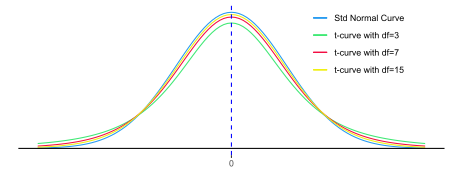
\includegraphics[width=\textwidth]{Figures/t-curves}

\begin{itemize}
\item
  The \(t\)-distributions form a family of curves, called
  \textbf{\(t\)-curves}, parameterized by the
  degrees of freedom.
\item
  The \(t\)-distribution has the following important properties.

  \begin{itemize}
  \item
    Similar to the standard normal curve, it is symmetric about
    0 and the total area under a \(t\)-curve is
    1.
  \item
    The \(t\)-distribution has slightly more variation
    (i.e.~\(t\)-curves are slightly ``fatter'') than the
    standard normal distribution.
  \item
    When the degree of freedom increases, the
    \(t\)-distribution becomes closer to the standard normal
    distribution.
  \end{itemize}
\end{itemize}

\hypertarget{confidence-intervals-for-a-mean-with-unknown-population-sd}{%
\subsection{\texorpdfstring{Confidence Intervals for a Mean with
\textbf{Unknown} Population
SD}{Confidence Intervals for a Mean with Unknown Population SD}}\label{confidence-intervals-for-a-mean-with-unknown-population-sd}}

\begin{itemize}
\item
  Suppose the population is approximately normally distributed or not highly skewed with large sample size.
  At the confidence level \(1-\alpha\), the margin of error is
  \(E=t_{\alpha/2}\frac{s}{\sqrt{n}},\) and the confidence interval for
  a population mean \(\mu\) is
  \[\left[\bar{x}-t_{\alpha/2}\frac{s}{\sqrt{n}}, \bar{x}+t_{\alpha/2}\frac{s}{\sqrt{n}}\right],\]
  where \(t_{\alpha/2}\) is the critical value such that
  \(P(T<t_{\alpha/2})=1-\alpha/2\) for a Student \(t\)-distribution with
  degree of freedom \(n-1\).
\item
  In Excel, the critical value \(t_{\alpha/2}\) can be calculated by\\
  \texttt{T.INV((1+confidence\ level)/2,\ n-1)} or\\
  \texttt{T.INV.2T(1-confidence\ level,\ n-1)},\\ where \(n\) is the
  sample size.
\item
  The marginal error \(E=t_{\alpha/2}\frac{s}{\sqrt{n}}\) can also be
  obtained by the Excel function\\
  \texttt{CONFIDENCE.T(1-confidence\ level,\ s,\ n)}.
\end{itemize}

\begin{example}

A sample of size 15 drawn from a normally distributed population. Find
the critical value \(t_{\alpha/2}\) needed in construction of a
confidence interval:

\begin{enumerate}
\item
  when the level of confidence is 99\%;
\item
  when the level of confidence is 95\%.
\end{enumerate}

\end{example}
\vspace*{3\baselineskip}

\begin{example}

A sample of size 16 is randomly drawn from a normally distributed
population. The sample has a mean 79 and standard deviation 7. Construct
a confidence interval for that population mean at the 90\% level of
confidence.

\end{example}
\vspace*{7\baselineskip}

\begin{example}

The data blow shows numbers of hours worked from 40 randomly selected
employees from several grocery stores in the county.

30, 26, 33, 26, 26, 33, 31, 31, 21, 37, 27, 20, 34, 35, 30, 24, 38, 34, 39, 31,\\
22, 30, 23, 23, 31, 44, 31, 33, 33, 26, 27, 28, 25, 35, 23, 32, 29, 31, 25, 27

Construct 99\% confidence interval for the mean worked time.

\end{example}
\vspace*{10\baselineskip}

\hypertarget{choose-between-normal-distribution-and-t-distribution}{%
\subsection{\texorpdfstring{Choose Between Normal Distribution and
\(t\)-Distribution}{Choose Between Normal Distribution and t-Distribution}}\label{choose-between-normal-distribution-and-t-distribution}}

\begin{itemize}
\item
  Population is approximately normally distributed.

  \begin{itemize}
  \item
    the population standard deviation \(\sigma\) is known:
    use the normal distribution.
  \item
    the population standard deviation \(\sigma\) is
    \emph{unknown}: use the
    \(t\)-\emph{distribution}.
  \end{itemize}
\item
  Population distribution unknown but \textbf{not highly skewed}. If the \textbf{sample size is large}
  enough, i.e.~\(n>30\), then

  \begin{itemize}
  \item
    the population standard deviation \(\sigma\) is known:
    use normal distribution.
  \item
    the population standard deviation \(\sigma\) is
    \emph{unknown}: either one can be used but the
    \(t\)-\emph{distribution} is more accurate.
  \end{itemize}
\item
  \textbf{Warning:} When the population distribution is unknown and the
  sample size is small, neither the \(t\)-distribution nor the
  normal distribution is reliable.
\item
  For small samples, there is method called
  ``\href{http://www.sthda.com/english/wiki/normality-test-in-r\#normality-test}{The
  Shapiro--Wilk test}'' which can be used to determine if we may assume
  the sampling distribution is approximately normal.
\item
  Even when \(n>30\), a visual inspection (using histogram for example)
  of the normality is necessary.
\end{itemize}

\hypertarget{practice}{%
\subsection{Practice}\label{practice}}

\begin{exercise}

Decide whether the following statements are true or false. Explain your
reasoning.

\begin{itemize}
\item
  The statement, ``the 95\% confidence interval for the population mean
  is (350, 400)'' means that 95\% of the population values are between
  350 and 400.
\item
  For a given standard error, lower confidence levels produce wider
  confidence intervals.
\item
  If you increase sample size, the width of confidence intervals will
  increase.
\item
  If you take large random samples over and over again from the same
  population, and make 95\% confidence intervals for the population
  average, about 95\% of the intervals should contain the population
  average.
\end{itemize}
\end{exercise}

\begin{exercise}

A sample of 34 watermelons' have a mean weight of 64 ounces. Assume the
population standard deviation is 12.7 ounces. Based on this, what is the
maximal margin of error associated with a 90\% confidence interval for
the true population mean watermelon weight.

\end{exercise}
\vspace*{8\baselineskip}

\begin{exercise}

If a school district takes a random sample of 70 Math SAT scores and
finds that the average is 426, and knowing that the population standard
deviation of Math SAT scores is intended to be 100. Find a 99\%
confidence interval for the mean math SAT score for this district.

\end{exercise}
\vspace*{8\baselineskip}

\begin{exercise}

In a survey, 32 people were asked how much they spent on their child's
last birthday gift. The results were roughly bell-shaped with a mean of
\$39 and standard deviation of \$7. Find the margin of error at a 80\%
confidence level.

\end{exercise}
\vspace*{8\baselineskip}

\begin{exercise}

A statistics student is curious about drinking habits of students at his
college. He wants to estimate the mean number of alcoholic drinks
consumed each week by students at his college. He plans to use a 90\%
confidence interval. He surveys a random sample of 71 students. The
sample mean is 3.93 alcoholic drinks per week. The sample standard
deviation is 3.78 drinks.

\end{exercise}
\vspace*{8\baselineskip}

\begin{exercise}

Four hundred randomly selected working adults in a certain state,
including those who worked at home, were asked the distance from their
home to their workplace. The average distance was 8.84 miles with
standard deviation 2.70 miles.

Construct a 98\% confidence interval for the mean distance from home to
work for all residents of this state.

\end{exercise}
\vspace*{8\baselineskip}

\begin{exercise}

City planners wish to estimate the mean lifetime of the most commonly
planted trees in urban settings. A sample of 16 recently felled trees
yielded mean age 32.7 years with standard deviation 3.1 years. Assuming
the lifetimes of all such trees are normally distributed, construct a
99.8\% confidence interval for the mean lifetime of all such trees.

\end{exercise}
\vspace*{8\baselineskip}

\begin{exercise}

Assuming the the population is normally distributed, find the 90\% confidence interval for the population mean using the following sample.

45.8, 56.8, 65, 67.5, 30.4, 43.9, 59.7, 51.3

\end{exercise}
\vspace*{8\baselineskip}

\hypertarget{lab-confidence-intervals}{%
\subsection{Lab: Confidence Intervals}\label{lab-confidence-intervals}}

\subsubsection{Excel Functions for
\(t\)-Distributions}

Suppose a Student's \(t\)-distribution has the degree of freedom
\(\text{df}=n-1\).

\begin{itemize}
\item
  Find a probability for a given \(t\)-value.

  \begin{itemize}
  \item
    The area of the left tail of the \(t\)-value may be calculated by
    the function \texttt{T.DIST(t,df,true)}.
  \item
    The area of the right tail of the \(t\)-value may be calculated by
    the function \texttt{T.DIST.RT(t,df)}.
  \item
    The area of two tails of the \(t\)-value (here \(t\)> 0)
    may be calculated by function \texttt{T.DIST.2T(t,df)}.
  \end{itemize}
\item
  Find the critical value for a given probability \(p\).

  \begin{itemize}
  \item
    When the area of the left tail is given, the function
    \texttt{T.INV(p,df)} may be used.
  \item
    When the area of both tails is given, the function\\
    \texttt{T.INV.2T(p,df)}\\
    may be used. This function is good for
    construction confidence interval.
  \end{itemize}
\end{itemize}

\hypertarget{excel-functions-for-marginal-errors}{%
\subsubsection{Excel Functions for Marginal
Errors}\label{excel-functions-for-marginal-errors}}

\begin{itemize}
\item
  If the population standard deviation \(\sigma\) is given and the
  sampling distribution is approximately normal, the marginal error can be obtained by the Excel function\\
  \begin{fullwidth}
    \colorbox{white}{
      \texttt{CONFIDENCE.NORM(1-confidence\ level,\ population\ SD,\ sample\ size)}
    }
  \end{fullwidth}
\item
  If the population standard deviation \(\sigma\) is NOT given and the
  sampling distribution is approximately normal, the marginal error can
  be obtained by the Excel function, the marginal error can be obtained by the Excel function

  \begin{fullwidth}
    \colorbox{white}{
      \texttt{CONFIDENCE.T(1-confidence\ level,\ sample\ SD,\ sample\ size)}
    }
  \end{fullwidth}
\end{itemize}

\begin{exercise}

A sample of size 28 randomly selected to estimate a population mean with
a confidence interval. The population is approximately normally
distributed.

Find the critical value that corresponds to a confidence level of 80\%.

\end{exercise}
\vspace*{6\baselineskip}

\begin{exercise}

A sample of 22 backpacks' have a mean weight of 77 ounces. Assume the
population standard deviation is 11.3 ounces. Based on this, what is the
maximal margin of error associated with a 95\% confidence interval for
the true population mean backpack weight.

\end{exercise}
\vspace*{6\baselineskip}

\begin{exercise}

In a survey, 21 people were asked how much they spent on their child's
last birthday gift. The results were roughly bell-shaped with a mean of
\$34 and standard deviation of \$6. Find the margin of error at a 98\%
confidence level.

\end{exercise}
\vspace*{6\baselineskip}

\begin{exercise}

Assuming the the population is normally distributed. Find the 99.5\%
confidence interval for the population mean using the following sample.

97.8, 90.4, 76.9, 88.6, 97.1, 87.8, 88, 69.9, 75.3, 81.6

\end{exercise}
\vspace*{6\baselineskip}


\newlecture

% !TeX root = main.tex

\hypertarget{confidence-interval-for-a-proportion}{%
\subsection{Confidence Interval for a
Proportion}}

\begin{itemize}
\item
  Recall that the standard error of sample proportions is
  \(\sigma_{\hat{P}}=\sqrt{\frac{p(1-p)}{n}}\), where \(n\) is the
  sample size and \(p\) is the population proportion. As a consequence,
  when estimating the population proportion \(p\), we only have a point
  estimate \(\hat{p}\) (phat) to use. For the standard error, we use the
  estimation
  \[\sigma_{\hat{p}}\approx\hat{\sigma}_{\hat{p}}=\sqrt{\dfrac{\hat{p}(1-\hat{p})}{n}}.\]

\item
  Based on the central limit theorem, when \(n\) is large enough, at the
  \(100(1-\alpha)\%\) level, the margin of error for \(p\) is defined as
  \[E=z_{\alpha/2}\sqrt{\frac{\hat{p}(1-\hat{p})}{n}}\]
  In Excel,\\
  \begin{fullwidth}\raggedleft
    \colorbox{white}{
      \(z_{\alpha/2}\)=\texttt{NORM.S.INV((1\ +\ confidence\ level)/2)}.
  
      \footnote{\footnotesize
        By the central limit theorem, the random variable \(\hat{p}\) is
      normal distributed. The chance that
      \[p\in \left[\hat{p}-z_{\alpha/2}\sqrt{\frac{\hat{p}(1-\hat{p})}{n}}, \hat{p}+z_{\alpha/2}\sqrt{\frac{\hat{p}(1-\hat{p})}{n}}\right]\]
      is the same as the chance that
      \[\hat{p}\in \left[p-z_{\alpha/2}\sqrt{\frac{p(1-p)}{n}}, p+z_{\alpha/2}\sqrt{\frac{p(1-p)}{n}}\right].\]
      That shows \(z_{\alpha/2}\) satisfying
      \[P(-z_{\alpha/2}<\dfrac{\hat{p}-p}{\sqrt{\frac{p(1-p)}{n}}}<z_{\alpha/2})=1-\alpha.\]
      }
    }
  \end{fullwidth}

  The marginal error can also be obtained by

  \begin{fullwidth}
    \colorbox{white}{
      \texttt{CONFIDENCE.NORM(1-confidence\ level,\ SQRT(phat*(1-phat)/n,\ n)}.
    }
  \end{fullwidth}

\item
  The confidence interval for \(p\) is defined by
  \[[\hat{p}-E,\hat{p}+E]=\left[\hat{p}-z_{\alpha/2}\sqrt{\frac{\hat{p}(1-\hat{p})}{n}}, \hat{p}+z_{\alpha/2}\sqrt{\frac{\hat{p}(1-\hat{p})}{n}}\right],\]
  where
  \href{https://saylordotorg.github.io/text_introductory-statistics/s11-01-large-sample-estimation-of-a-p.html}{the
  critical value \(z_{\alpha/2}\) satisfies that
  \(P(Z< z_{\alpha/2})=1-\alpha/2\)} for the standard normal variable
  \(Z\).
\item
  In practical, the sample size \(n\) is considered large enough if
  \(n\hat{p}\ge 10\) and \(n(1-\hat{p})\ge 10\).
\item
  The above defined confidence interval is known as the
  \href{https://en.wikipedia.org/wiki/Binomial_proportion_confidence_interval}{normal
  approximation (or Wald's) confidence interval}. It is popular in
  introductory statistics books. However, it is unreliable when the
  sample size is small or the sample proportion is close to 0 or 1.
  Indeed, if the sample proportion is 0 or 1, the confidence interval
  defined here will have zero length.
\end{itemize}



\begin{example}

In a random sample of 100 students in college, 65 said that they come to
college by bus.

\begin{enumerate}
\item
  Give a point estimate of the proportion of all students who come to
  college by bus.
\item
  Construct a 99\% confidence interval for that proportion.
\end{enumerate}

\end{example}
\vspace*{4\baselineskip}

\begin{example}
  
  Foothill College's athletic department wants to calculate the proportion
  of students who have attended a women's basketball game at the college.
  They use student email addresses, randomly choose 220 students, and
  email them. Of the 145 who responded, 22 had attended a women's
  basketball game.
  
  Calculate and interpret the approximate 90\% confidence interval for the
  proportion of all Foothill College students who have attended a women's
  basketball game.
  
\end{example}
\vspace*{8\baselineskip}


\subsection{Factors Affect the Width of Confidence
Intervals}

\begin{itemize}
\item
  The width of a confidence interval, equals twice the standard error,
  gives a measure of precision of the estimation.
\item
  Recall, for population proportion and mean,
  \[\text{Marginal Error} = \text{Critical Value}\cdot \frac{\text{(estimated) Population SD}}{\sqrt{\text{Sample Size}}}\]
\item
  The formula tells us the precision of a confidence interval is
  affected by the confidence level, the variability, and the sample
  size.

  \begin{itemize}
  \item
    Larger the confidence levels give larger critical values and errors.
  \item
    Populations (and samples) with more variability gives larger errors.
  \item
    Larger sample sizes give smaller errors.
  \end{itemize}
\end{itemize}

\hypertarget{sample-size-determination}{%
\subsection{Sample Size Determination}\label{sample-size-determination}}

\begin{itemize}
\item
  In practice, we may desire a marginal error of \(E\). With a fixed
  confidence level \(100(1-\alpha)\%\), the larger the sample size the
  smaller the marginal error.
\item
  When estimating population proportion, if we can produce a reasonable
  guess \(\hat{p}\) for population proportion, then an appropriate
  minimum sample size for the study is determined by
  \[n=\left(\frac{z_{\alpha/2}}{{E}}\right)^2\cdot \hat{p}(1-\hat{p}).\]
\item
  When estimating population mean, if we can produce a reasonable guess
  \(\sigma\) for the population standard deviation, then an appropriate
  minimum sample size is given by
  \[n=\left(\dfrac{z_{\alpha/2}\cdot \sigma}{{E}}\right)^2.\]
\end{itemize}

\begin{example}

Suppose you want to estimate the proportion of students at QCC who live
in Queens. By surveying your classmates, you find around 70\% live in
Queens. Use this as a guess to determine how many students would need to
be included in a random sample if you wanted the error of margin for a
95\% confidence interval to be less than or equal to 2\%.

\end{example}
\vspace*{8\baselineskip}

\begin{example}

Find the minimum sample size necessary to construct a 99\% confidence
interval for the population mean with a margin of error \(E =0.2\).
Assume that the estimated population standard deviation is
\(\sigma=1.3\).

\end{example}
\vspace*{8\baselineskip}

\begin{exercise}

Out of 400 people sampled, 92 had kids. Based on this, construct a 90\%
confidence interval for the true population proportion of people with
kids.

\end{exercise}
\vspace*{8\baselineskip}

\begin{exercise}

To understand the reason for returned goods, the manager of a store
examines the records on 40 products that were returned in the last year.
Reasons were coded by 1 for ``defective,'' 2 for ``unsatisfactory,'' and
0 for all other reasons, with the results shown in the table.

\begin{fullwidth}
  \colorbox{white}{
    \parbox{\linewidth}{\raggedleft
      \begin{tabular}{*{20}{c}}
        0 & 0 & 0 & 0 & 2 & 0 & 0 & 0 & 0 & 0 & 2 & 0 & 0 & 0 & 0 & 0 & 0 & 0 & 0 & 0 \\
        0 & 0 & 0 & 1 & 0 & 0 & 0 & 0 & 2 & 0 & 2 & 0 & 0 & 0 & 0 & 0 & 0 & 2 & 0 & 0
      \end{tabular}
    }}
\end{fullwidth}

\begin{enumerate}
\item
  Give a point estimate of the proportion of all returns that are
  because of something wrong with the product, that is, either defective
  or performed unsatisfactorily.
\item
  Construct an 80\% confidence interval for the proportion of all
  returns that are because of something wrong with the product.
\end{enumerate}

\end{exercise}

\begin{exercise}

You want to obtain a sample to estimate a population mean. Based on
previous evidence, you believe the population standard deviation is
approximately $\sigma=41.5$. You would like to be
99\% confident that your esimate is within 0.5 of the true population
mean. How large of a sample size is required?

\end{exercise}
\vspace*{8\baselineskip}

\begin{exercise}

Suppose a mobile phone company wants to determine the current percentage
of customers aged 50+ who use text messaging on their cell phones. How
many customers aged 50+ should the company survey in order to be 90\%
confident that the estimated (sample) proportion is within three
percentage points of the true population proportion of customers aged
50+ who use text messaging on their cell phones.

\end{exercise}
\vspace*{8\baselineskip}

\subsection{Lab: Confidence Interval for Proportion}

\begin{itemize}
\item
  When a cumulative probability \(p=P(Z<z)\) of a standard normal random
  variable \(Z\) is given, we can find \(z\) using
  \texttt{NORM.S.INV(p)}.
\item
  If a sample of size \(n\) has the proportion \(\hat{p}\) and the
  sampling distribution is approximately normal, the marginal error for
  the proportion can be obtained by the Excel function
  \vskip 0.5em
  \begin{fullwidth}
    \colorbox{white}{
      \texttt{CONFIDENCE.NORM(1-confidence\ level,\ SQRT(phat*(1-phat)),\ n)}
    }
  \end{fullwidth}
\end{itemize}

\begin{exercise}
  
  Suppose 250 randomly selected people are surveyed to determine if they own a tablet. Of the 250 surveyed, 98 reported owning a tablet. Using a 95\% confidence level, compute a confidence interval estimate for the true proportion of people who own tablets.

\end{exercise}
\vspace*{8\baselineskip}

\begin{exercise}

A software engineer wishes to estimate, to within 5 seconds, the mean
time that a new application takes to start up, with 95\% confidence.
Estimate the minimum size sample required if the standard deviation of
start up times for similar software is 12 seconds.

\end{exercise}
\vspace*{8\baselineskip}

\begin{exercise}

The administration at a college wishes to estimate, to within two
percentage points, the proportion of all its entering freshmen who
graduate within four years, with 90\% confidence. Estimate the minimum
size sample required.

\end{exercise}
\vspace*{8\baselineskip}


\newlecture

% !TeX root = main.tex

\hypertarget{concepts-of-hypothesis-testing}{%
\section{Concepts of Hypothesis
Testing}\label{concepts-of-hypothesis-testing}}

\hypertarget{the-basic-idea-of-hypothesis-testing}{%
\subsection{The Basic Idea of Hypothesis
Testing}\label{the-basic-idea-of-hypothesis-testing}}

\begin{itemize}
\item
  The testing procedure starts with an initial assumption that the
  statement on population parameter is true.
\item
  We test this initial assumption using a random sample. If the initial
  assumption is really the truth, then the test statistic from a random
  sample shouldn't be too far away from the center of the sampling
  distribution. Conversely, if the test statistic is too far
  away from the center, then we should not believe in the
  initial assumption.
\item
  To determine how far is too far away, we need to specify a threshold,
  a prior probability, or equivalently a critical value.
\item
  If the test statistic is at least extreme as the critical value, then
  the testing is significant enough to allow us to reject the initial
  assumption. Otherwise, we cannot draw a definite conclusion.
\item
  The prior probability measures the chance that the initial assumption
  was wrongly rejected.
\end{itemize}

\hypertarget{two-hypotheses}{%
\subsection{Two Hypotheses}\label{two-hypotheses}}

\begin{itemize}
\item
  A statistical \textbf{hypothesis} is a statement about a population
  parameter.
\item
  A \textbf{hypothesis test} is a process that uses sample statistics to
  test a \textbf{hypothesis}.
\item
  To test a population parameter, we choose a pair of hypotheses, the
  null hypothesis and the alternative hypothesis which are contradictory
  to each other.
\item
  The \textbf{null hypothesis}, denoted by \(H_0\), is the statement
  about the population parameter that is assumed to be true.
\item
  The \textbf{alternative hypothesis}, denoted \(H_a\), is a statement
  about the population parameter that is contradictory to the null
  hypothesis.
\end{itemize}

\begin{fullwidth}
  \colorbox{white}{
    \parbox{\linewidth}{\centering
      \textbf{Mathematical Symbols Used in \(H_0\) and \(H_a\)}
      
      \begin{longtable}[]{@{}cc@{}}
      \toprule()
      \(H_0\) & \(H_a\) \\
      \midrule()
      \endhead
      equal = & not equal \(\neq\) or greater than $>$ or less than
      $<$\\
      greater than or equal to \(\geq\) & less than $<$ \\
      less than or equal to $\leq$ & more than $>$ \\
      \bottomrule()
      \end{longtable}
    }}
\end{fullwidth}

\begin{example}

Identify the Null and the Alternative Hypotheses

\begin{enumerate}
\item
  Test a statement that the population mean is 1.
\item
  Test a statement that the population mean is more than 3.
\item
  Test a statement that the population mean is no more than 3.
\end{enumerate}

\end{example}


\hypertarget{the-logic-of-hypothesis-testing}{%
\subsection{The Logic of Hypothesis
Testing}\label{the-logic-of-hypothesis-testing}}

The logic of hypothesis testing and two types of error can be summarized in the following table.

\begin{fullwidth}
  \colorbox{white}{
\parbox{\linewidth}{\centering
  \begin{tabular}{l|*{2}{l}}
    ACTION & $H_0$  is Actually True & $H_0$  is Actually False\\
    \midrule
    Do not reject  $H_0$ & 	Correct Outcome	 & Type II error\\
    Reject  $H_0$ &	Type I Error & Correct Outcome
  \end{tabular}
}
  }
\end{fullwidth}


The interpretation of hypothesis testing is summarized in the following
table.

\begin{fullwidth}
  \colorbox{white}{
\parbox{\linewidth}{\centering
\begin{tabular}{l|p{0.35\linewidth}p{0.35\linewidth}}
  Action & If the claim to be tested is in \(H_0\) & If the claim to be tested is in \(H_a\) \\
  \midrule
  Reject \(H_0\) & There is enough evidence to reject the claim
  & There is enough evidence to support the claim \\
  Fail to Reject \(H_0\) & There is not enough evidence to reject the claim & There is not enough evidence to support the claim
\end{tabular}
}
  }
\end{fullwidth}

\hypertarget{type-of-errors-in-hypothesis-testing}{%
\subsection{Type of Errors in Hypothesis
Testing}\label{type-of-errors-in-hypothesis-testing}}

\begin{itemize}
\item
  Rejecting the null hypothesis when it is indeed true is called a
  \textbf{type I error}. The maximum allowable probability of making a
  type I error is called the \textbf{level of significance}, denoted by
  \(\alpha\). In other words,
  \[\alpha=P(\text{Type I error})= P(\text{reject a true }H_0).\]
\item
  Failing to reject the null hypothesis when the it is false is called a
  \textbf{type II error}. The probability of a type II error is usually
  denoted by \(\beta\). The \textbf{power of a hypothesis test}, equals
  \(1-\beta\), is the probability of rejecting the null hypothesis when
  it is false.
\end{itemize}

\begin{example}
Examples of Type I and Type II errors
\begin{center}
  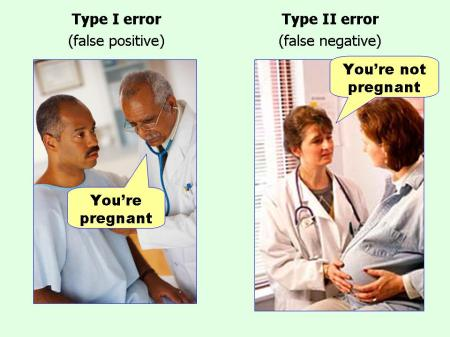
\includegraphics[width=0.9\textwidth]{Figures/type-i-and-type-ii-errors.jpg}\\
  \textbf{In the above picture, bubble texts are in \(H_a\)}
\end{center}
\end{example}
\vspace*{\baselineskip}

\hypertarget{type-of-tests}{%
\subsection{Type of Tests}\label{type-of-tests}}

\begin{itemize}
\item
  If \(H_a\) has the form \(\mu\neq \mu_0\) the test is called a
  \textbf{two-tailed test}.
\item
  If \(H_a\) has the form \(\mu<\mu_0\) the test is called a
  \textbf{left-tailed test}.
\item
  If \(H_a\) has the form \(\mu>\mu_0\) the test is called a
  \textbf{right-tailed test}.
\item
  Each of the last two forms is also called a \textbf{one-tailed test}.
\end{itemize}

\hypertarget{observed-significance}{%
\subsection{Observed Significance}\label{observed-significance}}

\begin{itemize}
\item
  To make a decision, one may also compare probabilities. The
  \textbf{observed significance} (\textbf{$P$-value}) of a test statistic is the probability of obtaining a sample statistic at least as extreme as the (observed) test statistic, given that the null hypothesis were true.
\item
  \(P\)-Value as Tail area

  \begin{longtable}[]{@{}lcc@{}}
  \toprule()
  Sign in \(H_a\) & \(\ne\) & \(<\) \\
  \midrule()
  \endhead
  \(P\)-value & Double of the tail area & Left tail area \\
  \bottomrule()
  \end{longtable}
\item
  Making decision by comparing the \(P\)-value with the significance
  level \(\alpha\):

  \begin{itemize}
  \item
    reject \(H_0\) if \(p\le \alpha\)
  \item
    fail to reject \(H_0\) if \(p>\alpha\).
  \end{itemize}
\end{itemize}

\begin{example}

Given the following testing hypotheses

\(H_{0}: p=0.50\) vs.~\(H_{a}: p\ne 0.50, n=360, \hat{p}=0.56\),

find the \(P\)-value for the test and make a decision at the 5\% level
of significance.

\end{example}
\vspace*{8\baselineskip}

\begin{example}

It is believed that a stock price for a particular company will grow at
a rate of \$5 per week with a standard deviation of \$1. An investor
believes the stock won't grow as quickly. The changes in stock price is
recorded for ten weeks and are as follows: \$4, \$3, \$2, \$3, \$1, \$7,
\$2, \$1, \$1, \$2. State the null and alternative hypotheses, find the
p-value, and identify the Type I and Type II errors.

\end{example}
\vspace*{8\baselineskip}

\hypertarget{hypothesis-testing-procedure}{%
\subsection{Hypothesis Testing
Procedure}\label{hypothesis-testing-procedure}}

\begin{enumerate}[sepno]
\item
  Check if the population distribution is approximately normal or sample size is large enough and determine if a \(Z\)-test
  or \(T\)-test can be performed. For proportion, \(Z\)-test may be
  used. For mean, if \(\sigma\) is known, the \(Z\)-test may be used. If
  \(\sigma\) is unknown, the \(T\)-test may be used.
\item
  State the null and alternative hypothesis. The null hypothesis always
  contains the equal sign (and possibly together with a less than or
  greater than symbol, depending on \(H_a\).)
\item
  Set a significance level \(\alpha\). Commonly used levels are
  \(\alpha=0.01\), \(\alpha=0.05\) and \(\alpha=0.1\).
\item
  Calculate the standardized test statistic: the \(Z\)-test statistic or
  the \(T\)-test statistic.
\item
  Calculate the \(P\)-value according to the type of the test.

  \begin{tabular}{cc}
    \toprule
    Sign in \(H_a\) & Type of Test\\
    \midrule
    \(\ne\) & Two-tailed\\
    \(<\) &  Left-tailed\\
    \(>\) & Right-tailed\\
    \bottomrule
  \end{tabular}
  
\item
  Make a test decision about the null hypothesis \(H_0\). We reject
  \(H_0\) if the \(P\)-value less than the significance level
  \(\alpha\).
\item
  State an overall conclusion.
\end{enumerate}
\vspace*{-0.5\baselineskip}

\begin{example}

Residences on a certain street claim that the mean speed of automobiles
run through the street is greater than the speed limit of 25 miles per
hour. A random sample of 100 automobiles has a mean speed of 26 miles
per hour. Assume the population standard deviation is 4 miles per hour.
Is there enough evidence to support the claim of the residences at the
significance level \(\alpha = 0.05\)?

\end{example}
\vspace*{8\baselineskip}

\begin{example}

A certain manufacturer claims that average numbers of candies in a
certain sized bag that they produce is 20. To test the claims, you
collected a random sample of 10 bags and find the mean is 18 and the
standard deviation is 2.7. Assume the numbers of candies are normally
distributed. At the significance level \(\alpha=0.05\), does your
analysis support the manufacturer's claim?

\end{example}
\vspace*{8\baselineskip}

\begin{example}

An instructor would like to know if the students enrolled in a math
course in the current semester performed better than students in the
last semester. The mean final exam from last semester is 75.5. The final
exam scores of 40 randomly selected 40 students were obtained

\begin{fullwidth}
  \colorbox{white}{
    \parbox{\linewidth}{
      \raggedleft
      \begin{tabular}{*{20}{c}}
        93 & 88 & 69 & 74 & 76 & 81 & 78 & 77 & 74 & 63 & 67 & 81 & 80 & 82 & 68 & 88 & 76 & 69 & 75 & 78\\
        75 & 77 & 94 & 87 & 74 & 88 & 63 & 75 & 94 & 88 & 91 & 77 & 76 & 68 & 80 & 88 & 68 & 83 & 72 & 72
      \end{tabular}
    }
  }
\end{fullwidth}

Do the data provide evidence that the students in this semester
performed significantly better on the final than last semester?

\end{example}
\vspace*{8\baselineskip}

\begin{example}

Suppose you want to determine if a coin is fair. You toss the coin 50
times and observe 16 heads and 34 tails. At the significant level 0.01,
do you think that the coin is fair? If not, does the coin favor the head
or tail?

\end{example}
\vspace*{8\baselineskip}

\begin{example}

Globally the long-term proportion of newborns who are male is 51.46\%. A
researcher believes that the proportion of boys at birth changes under
severe economic conditions. To test this belief randomly selected birth
records of 5,000 babies born during a period of economic recession were
examined. It was found in the sample that 52.55\% of the newborns were
boys. Determine whether there is sufficient evidence, at the 10\% level
of significance, to support the researcher's belief.

\end{example}
\vspace*{8\baselineskip}

\begin{remark}

In some books, the standard error of the sample distribution of sample
proportions assuming that \(p=p_0\) is calculated using the
approximation \[
\sigma_{\hat{p}}=\sqrt{\frac{\hat{p}(1-\hat{p})}{n}}.
\]

An arguable explanation is that using the above value for SE will be
consistent with the approach to a hypothesis testing using a confidence
interval in the case that a two-tailed test is preformed.

\end{remark}

\begin{example}

  The mean work week for engineers in a start-up company is believed to be
  about 60 hours. A newly hired engineer hopes that it's shorter. She asks
  ten engineering friends in start-ups for the lengths of their mean work
  weeks. Based on the results that follow, should she count on the mean
  work week to be shorter than 60 hours?
  
  Data (length of mean work week): 70; 45; 55; 60; 65; 55; 55; 60; 50; 55.
  
\end{example}
\vspace*{8\baselineskip}


\hypertarget{practice}{%
\subsection{Practice}\label{practice}}

\begin{exercise}

Decide whether the following statements are true or false. Explain your reasoning.

\begin{itemize}
\item
  In case of a left-tailed test, we reject the null hypothesis if the
  sample statistic is significantly smaller than the hypothesized
  population parameter.
\item
  A \(P\)-value of 0.08 is more evidence against the null hypothesis
  than a \(P\)-value of 0.04.
\item
  The statement, ``the \(P\)-value is 0.03'', is equivalent to the
  statement, ``there is a 3\% probability that the null hypothesis is
  true''.
\item
  Even though you rejected the null hypothesis, it may still be true.
\item
  Failing to reject null hypothesis means the null hypothesis is true.
\item
  That the \(P\)-value of a sample statistic is \(p=0\) means the null
  hypothesis cannot be true.
\end{itemize}

\end{exercise}
\vspace*{4\baselineskip}

\begin{exercise}

Determine both Type I and Type II errors for the following scenario:

Assume a null hypothesis, \(H_0\), that states the percentage of adults
with jobs is at least 88\%. Identify the Type I and Type II errors from
these four statements.

\begin{enumerate}
\item
  Not to reject the null hypothesis that the percentage of adults who
  have jobs is at least 88\% when that percentage is actually less than
  88\%
\item
  Not to reject the null hypothesis that the percentage of adults who
  have jobs is at least 88\% when the percentage is actually at least
  88\%.
\item
  Reject the null hypothesis that the percentage of adults who have jobs
  is at least 88\% when the percentage is actually at least 88\%.
\item
  Reject the null hypothesis that the percentage of adults who have jobs
  is at least 88\% when that percentage is actually less than 88\%.
\end{enumerate}

\end{exercise}
\vspace*{2\baselineskip}

\begin{exercise}

  Determine if the following statements are true or false. Please explain your reasoning.

  \begin{itemize}
  \item
    The \(P\)-value of the test statistic is \(p = 0.06\). At the
    significance level \(\alpha=0.01\), the null hypothesis \(H_0\)
    should be rejected.
  \item
    A two-tailed test has larger probability of getting a type I error
    that a one-tailed test.
  \item
    That a test statistic falls in the rejection region means the
    \(P\)-value is smaller than the significance level.
  \end{itemize}

\end{exercise}
\vspace*{4\baselineskip}

\begin{exercise}

Suppose we're conducting a hypothesis testing for a population mean.
Find the \(P\)-value for each of the following testing scenario with the
given sample size \(n\) and the test statistics \(t\).

\begin{enumerate}
\item
  \(H_{0}: \mu=25 \text { vs. } H_{a} : \mu<25\), \(n=30\), \(t=-2.43\).
\item
  \(H_{0}: \mu=35 \text { vs. } H_{a} : \mu>35\), \(n=50\), \(t=2.13\).
\item
  \(H_{0}: \mu=-7.9 \text { vs. } H_{a} : \mu\ne-7.9\), \(n=40\),
  \(t=-1.99\).
\end{enumerate}

\end{exercise}

\begin{exercise}

It's a Boy Genetics Labs claim their procedures improve the chances of a
boy being born. The results for a test of a single population proportion
are as follows:

\begin{itemize}
\item
  \(H_0: p=0.50\), \(H_a:p>0.50\)
\item
  \(\alpha=0.01\)
\item
  \(p-\text{value}=0.025\)
\end{itemize}

Interpret the results and state a conclusion in simple, non-technical
terms.

\end{exercise}

\vspace*{8\baselineskip}


\begin{exercise}

A college football coach thought that his players could bench press a
mean weight of 275 pounds. It is known that the standard deviation is 55
pounds. Three of his players thought that the mean weight was more than
that amount. They asked 30 of their teammates for their estimated
maximum lift on the bench press exercise. The mean of their maximum lift
is 286.2.

Conduct a hypothesis test using a 2.5\% level of significance to
determine if the bench press mean is more than 275 pounds.

\end{exercise}
\vspace*{8\baselineskip}

\begin{exercise}

In a college report, it says the mean age of students is 23.4 years old.
An instructor thinks that the mean age is younger than 23.4. He randomly
surveyed 50 students and found that the sample mean is 21.5 and the
standard deviation is 1.9. At the significance level \(\alpha=0.025\),
is there enough evidence to support the instructor's estimation?

\end{exercise}
\vspace*{8\baselineskip}

\begin{exercise}

A teacher believes that 85\% of students in the class will want to go on
a field trip to the local zoo. She performs a hypothesis test to
determine if the percentage is the same or different from 85\%. The
teacher samples 50 students and 39 reply that they would want to go to
the zoo. For a 1\% level of significance, would the data support the
teacher's believe?

\end{exercise}
\vspace*{8\baselineskip}

\begin{exercise}

  The average number of days to complete recovery from a particular type
  of knee operation is 123.7 days. From his experience a physician
  suspects that use of a topical pain medication might be lengthening the
  recovery time. He randomly selects the records of seven knee surgery
  patients who used the topical medication. The times to total recovery
  were:
  
  128, 135, 121, 142, 126, 151, 123
  
  Assuming a normal distribution of recovery times, perform the relevant
  test of hypotheses at the 10\% level of significance.
  
  Would the decision be the same at the 5\% level of significance?
  
  \end{exercise}
  \vspace*{8\baselineskip}

\hypertarget{lab-excel-functions-for-normal-distributions}{%
\subsection{Lab: Excel Functions for Normal
Distributions}\label{lab-excel-functions-for-normal-distributions}}

\begin{itemize}
\item
  Let \(Z\) be a standard normal random varaible. In Excel, \(P(Z<z)\)
  is given by \texttt{NORM.S.DIST(z,TRUE)}.
\item
  Let \(X\) be a normal random variable with mean \(\mu\) and standard
  deviation \(\sigma\), that is \(X\sim \mathcal{N}(\mu, \sigma^2)\). In
  Excel, \(P(X<x)\) is given by \texttt{NORM.DIST(x,mean,sd,TRUE)}.
\item
  When a cumulative probability \(p=P(X<x)\) of a normal random variable
  \(X\) is given, we can find \(x\) using\\ \texttt{NORM.INV(p,mean,sd)}.
\item
  When a cumulative probability \(p=P(Z<z)\) of a standard normal random
  variable \(Z\) is given, we can find \(z\) using
  \texttt{NORM.S.INV(p)}.
\end{itemize}

\hypertarget{lab-excel-functions-for-t-distributions}{%
\subsection{\texorpdfstring{Lab: Excel Functions for
\(T\)-Distributions}{Lab: Excel Functions for T-Distributions}}\label{lab-excel-functions-for-t-distributions}}

Suppose a Student's \(T\)-distribution has the degree of freedom
\(\text{df}=n-1\).

How to find a probability for a given \(T\)-value?

\begin{itemize}
  \item
    The area of the left tail of the \(T\)-value may be calculated by
    the function \texttt{T.DIST(t,df,true)}.
  \item
    The area of the right tail of the \(T\)-value may be calculated by
    the function \texttt{T.DIST.RT(t,\ df)}.
  \item
    The area of two tails of the \(T\)-value
    (\(t > 0\)) may be calculated by
    function \texttt{T.DIST.2T(t,df)}.
  \end{itemize}
  
    % To find the critical value for a given probability \(p\)
  
    % \begin{itemize}
    % \item
    %   When the area of the left tail is given, the function\\
    %   \texttt{T.INV(p,df)} may be used.
    % \item
    %   When the area of both tails is given, the function\\
    %   \texttt{T.INV.2T(p,df)} may be used. This function is good for
    %   construction confidence interval.
    % \end{itemize}

\begin{exercise}

Joon believes that 50\% of first-time brides in the United States are
younger than their grooms. She performs a hypothesis test to determine
if the percentage is the same or different from 50\%. Joon samples 100
first-time brides and 53 reply that they are younger than their grooms.
For the hypothesis test, find the \(p\)-value.

\end{exercise}
\vspace*{8\baselineskip}

\begin{exercise}

The average McDonald's restaurant generates \$3.7 million in sales each
year with a standard deviation of 0.7. Taylor wants to know if the
average sales generated by McDonald's restaurants in Missouri is greater
than the worldwide average. He surveys 24 restaurants in Missouri and
finds the following data (in millions of dollars):

\begin{tabular}{*{12}{c}}
  2.0 & 3.1 & 3.7 & 2.6 & 4.0 & 3.9 & 3.4 & 3.5 & 3.5 & 3.6 & 4.1 & 2.0 \\ 
  4.4 & 2.3 & 3.8 & 2.6 & 1.9 & 4.8 & 2.7 & 2.8 & 2.8 & 3.1 & 3.9 & 2.6  
\end{tabular}

Find the \(p\)-value.

\end{exercise}
\vspace*{8\baselineskip}

\begin{exercise}

The average number of days to complete recovery from a particular type
of knee operation is 123.7 days. From his experience a physician
suspects that use of a topical pain medication might be lengthening the
recovery time. He randomly selects the records of seven knee surgery
patients who used the topical medication. The times to total recovery
were:

128, 135, 121, 142, 126, 151, 123

Assuming a normal distribution of recovery times, perform the relevant
test of hypotheses at the 10\% level of significance.

Would the decision be the same at the 5\% level of significance?

\end{exercise}
\vspace*{8\baselineskip}
  

% \newlecture

% % !TeX root = main.tex

\hypertarget{hypothesis-testing-for-one-sample}{%
\section{Hypothesis Testing for One
Sample}\label{hypothesis-testing-for-one-sample}}

\hypertarget{hypothesis-testing-procedure}{%
\subsection{Hypothesis Testing
Procedure}\label{hypothesis-testing-procedure}}

\begin{enumerate}[sepno]
\item
  Check if the sample size is large enough and determine if a \(Z\)-test
  or \(T\)-test can be performed. For proportion, \(Z\)-test may be
  used. For mean, if \(\sigma\) is known, the \(Z\)-test may be used. If
  \(\sigma\) is unknown, the \(T\)-test may be used.
\item
  State the null and alternative hypothesis. The null hypothesis always
  contains the equal sign (and possibly together with a less than or
  greater than symbol, depending on \(H_a\).)
\item
  Set a significance level \(\alpha\). Commonly used levels are
  \(\alpha=0.01\), \(\alpha=0.05\) and \(\alpha=0.1\).
\item
  Calculate the standardized test statistic: the \(Z\)-test statistic or
  the \(T\)-test statistic.
\item
  Calculate the \(P\)-value according to the type of the test.

  \begin{tabular}{cc}
    \toprule
    Sign in \(H_a\) & Type of Test\\
    \midrule
    \(\ne\) & Two-tailed\\
    \(<\) &  Left-tailed\\
    \(>\) & Right-tailed\\
    \bottomrule
  \end{tabular}
  
\item
  Make a test decision about the null hypothesis \(H_0\). We reject
  \(H_0\) if the \(P\)-value less than the significance level
  \(\alpha\).
\item
  State an overall conclusion.
\end{enumerate}
\vspace*{-0.5\baselineskip}

\begin{example}

Residences on a certain street claim that the mean speed of automobiles
run through the street is greater than the speed limit of 25 miles per
hour. A random sample of 100 automobiles has a mean speed of 26 miles
per hour. Assume the population standard deviation is 4 miles per hour.
Is there enough evidence to support the claim of the residences at the
significance level \(\alpha = 0.05\)?

\end{example}
\vspace*{6\baselineskip}

\begin{example}

A certain manufacturer claims that average numbers of candies in a
certain sized bag that they produce is 20. To test the claims, you
collected a random sample of 10 bags and find the mean is 18 and the
standard deviation is 2.7. Assume the numbers of candies are normally
distributed. At the significance level \(\alpha=0.05\), does your
analysis support the manufacturer's claim?

\end{example}
\vspace*{8\baselineskip}

\begin{example}

An instructor would like to know if the students enrolled in a math
course in the current semester performed better than students in the
last semester. The mean final exam from last semester is 75.5. The final
exam scores of 40 randomly selected 40 students were obtained

\begin{fullwidth}
  \colorbox{white}{
    \parbox{\linewidth}{
      \raggedleft
      \begin{tabular}{*{20}{c}}
        93 & 88 & 69 & 74 & 76 & 81 & 78 & 77 & 74 & 63 & 67 & 81 & 80 & 82 & 68 & 88 & 76 & 69 & 75 & 78\\
        75 & 77 & 94 & 87 & 74 & 88 & 63 & 75 & 94 & 88 & 91 & 77 & 76 & 68 & 80 & 88 & 68 & 83 & 72 & 72
      \end{tabular}
    }
  }
\end{fullwidth}

Do the data provide evidence that the students in this semester
performed significantly better on the final than last semester?

\end{example}
\vspace*{8\baselineskip}

\begin{example}

Suppose you want to determine if a coin is fair. You toss the coin 50
times and observe 16 heads and 34 tails. At the significant level 0.01,
do you think that the coin is fair? If not, does the coin favor the head
or tail?

\end{example}
\vspace*{8\baselineskip}

\begin{example}

Globally the long-term proportion of newborns who are male is 51.46\%. A
researcher believes that the proportion of boys at birth changes under
severe economic conditions. To test this belief randomly selected birth
records of 5,000 babies born during a period of economic recession were
examined. It was found in the sample that 52.55\% of the newborns were
boys. Determine whether there is sufficient evidence, at the 10\% level
of significance, to support the researcher's belief.

\end{example}
\vspace*{8\baselineskip}

\begin{remark}

In some books, the standard error of the sample distribution of sample
proportions assuming that \(p=p_0\) is calculated using the
approximation \[
\sigma_{\hat{p}}=\sqrt{\frac{\hat{p}(1-\hat{p})}{n}}.
\]

An arguable explanation is that using the above value for SE will be
consistent with the approach to a hypothesis testing using a confidence
interval in the case that a two-tailed test is preformed.

\end{remark}

\begin{example}

  The mean work week for engineers in a start-up company is believed to be
  about 60 hours. A newly hired engineer hopes that it's shorter. She asks
  ten engineering friends in start-ups for the lengths of their mean work
  weeks. Based on the results that follow, should she count on the mean
  work week to be shorter than 60 hours?
  
  Data (length of mean work week): 70; 45; 55; 60; 65; 55; 55; 60; 50; 55.
  
\end{example}
\vspace*{8\baselineskip}

\hypertarget{practice}{%
\subsection{Practice}\label{practice}}

\begin{exercise}

A college football coach thought that his players could bench press a
mean weight of 275 pounds. It is known that the standard deviation is 55
pounds. Three of his players thought that the mean weight was more than
that amount. They asked 30 of their teammates for their estimated
maximum lift on the bench press exercise. The mean of their maximum lift
is 286.2.

Conduct a hypothesis test using a 2.5\% level of significance to
determine if the bench press mean is more than 275 pounds.

\end{exercise}
\vspace*{8\baselineskip}

\begin{exercise}

In a college report, it says the mean age of students is 23.4 years old.
An instructor thinks that the mean age is younger than 23.4. He randomly
surveyed 50 students and found that the sample mean is 21.5 and the
standard deviation is 1.9. At the significance level \(\alpha=0.025\),
is there enough evidence to support the instructor's estimation?

\end{exercise}
\vspace*{8\baselineskip}

\begin{exercise}

A teacher believes that 85\% of students in the class will want to go on
a field trip to the local zoo. She performs a hypothesis test to
determine if the percentage is the same or different from 85\%. The
teacher samples 50 students and 39 reply that they would want to go to
the zoo. For a 1\% level of significance, would the data support the
teacher's believe?

\end{exercise}
\vspace*{8\baselineskip}

\begin{exercise}

Suppose a consumer group suspects that the proportion of households that
have three cell phones is 30\%. A cell phone company has reason to
believe that the proportion is not 30\%. Before they start a big
advertising campaign, they conduct a hypothesis test. Their marketing
people survey 150 households with the result that 43 of the households
have three cell phones.

\end{exercise}
\vspace*{8\baselineskip}

\begin{exercise}

The average household size in a certain region several years ago was
3.14 persons. A sociologist wishes to test, at the 5\% level of
significance, whether it is different now. Perform the test using the
information collected by the sociologist: in a random sample of 75
households, the average size was 2.98 persons, with sample standard
deviation 0.82 person.

\end{exercise}
\vspace*{8\baselineskip}

\begin{exercise}

The mean score on a 25-point placement exam in mathematics used for the
past two years at a large state university is 14.3. The placement
coordinator wishes to test whether the mean score on a revised version
of the exam differs from 14.3. She gives the revised exam to 30 entering
freshmen early in the summer; the mean score is 14.6 with standard
deviation 2.4. Perform the test at the 10\% level of significance.

\end{exercise}
\vspace*{8\baselineskip}

\begin{exercise}

The average number of days to complete recovery from a particular type
of knee operation is 123.7 days. From his experience a physician
suspects that use of a topical pain medication might be lengthening the
recovery time. He randomly selects the records of seven knee surgery
patients who used the topical medication. The times to total recovery
were:

128, 135, 121, 142, 126, 151, 123

Assuming a normal distribution of recovery times, perform the relevant
test of hypotheses at the 10\% level of significance.

Would the decision be the same at the 5\% level of significance?

\end{exercise}
\vspace*{8\baselineskip}

\hypertarget{lab-excel-functions-for-hypothesis-testing}{%
\subsection{Lab: Excel Functions for Hypothesis
Testing}\label{lab-excel-functions-for-hypothesis-testing}}

\hypertarget{excel-functions-for-normal-distributions}{%
\subsubsection{Excel Functions for Normal
Distributions}\label{excel-functions-for-normal-distributions}}

\begin{itemize}
\item
  Let \(Z\) be a standard normal random varaible. In Excel, \(P(Z<z)\)
  is given by \texttt{NORM.S.DIST(z,TRUE)}.
\item
  Let \(X\) be a normal random variable with mean \(\mu\) and standard
  deviation \(\sigma\), that is \(X\sim \mathcal{N}(\mu, \sigma^2)\). In
  Excel, \(P(X<x)\) is given by \texttt{NORM.DIST(x,mean,sd,TRUE)}.
\item
  When a cumulative probability \(p=P(X<x)\) of a normal random variable
  \(X\) is given, we can find \(x\) using\\ \texttt{NORM.INV(p,mean,sd)}.
\item
  When a cumulative probability \(p=P(Z<z)\) of a standard normal random
  variable \(Z\) is given, we can find \(z\) using
  \texttt{NORM.S.INV(p)}.
\end{itemize}

\hypertarget{excel-functions-for-t-distributions}{%
\subsubsection{\texorpdfstring{Excel Functions for
\(T\)-Distributions}{Excel Functions for T-Distributions}}\label{excel-functions-for-t-distributions}}

Suppose a Student's \(T\)-distribution has the degree of freedom
\(\text{df}=n-1\).

\begin{itemize}
\item
  To find a probability for a given \(T\)-value

  \begin{itemize}
  \item
    The area of the left tail of the \(T\)-value may be calculated by
    the function \texttt{T.DIST(t,df,true)}.
  \item
    The area of the right tail of the \(T\)-value may be calculated by
    the function \texttt{T.DIST.RT(t,\ df)}.
  \item
    The area of two tails of the \(T\)-value
    (\(t > 0\)) may be calculated by
    function \texttt{T.DIST.2T(t,df)}.
  \end{itemize}
\item
  To find the critical value for a given probability \(p\)

  \begin{itemize}
  \item
    When the area of the left tail is given, the function\\
    \texttt{T.INV(p,df)} may be used.
  \item
    When the area of both tails is given, the function\\
    \texttt{T.INV.2T(p,df)} may be used. This function is good for
    construction confidence interval.
  \end{itemize}
\end{itemize}

\begin{exercise}

The average number of days to complete recovery from a particular type
of knee operation is 123.7 days. From his experience a physician
suspects that use of a topical pain medication might be lengthening the
recovery time. He randomly selects the records of seven knee surgery
patients who used the topical medication. The times to total recovery
were:

128, 135, 121, 142, 126, 151, 123

Assuming a normal distribution of recovery times, perform the relevant
test of hypotheses at the 10\% level of significance.

Would the decision be the same at the 5\% level of significance?

\end{exercise}




\end{document}
